\section{Studio su pannelli simulati}
Al fine di analizzare i risultati ottenuti si sono confrontate 5 varianti della
\textit{RLPBWT}:
\begin{itemize}
  \item \textit{RLPBWT na\"{i}ve}
  \item \textit{RLPBWT con bitvector}
  \item \textit{RLPBWT con pannello completo e threshold}
  \item \textit{RLPBWT con pannello compresso (SLP) e threshold}
  \item \textit{RLPBWT con pannello compresso (SLP) e LCE query}  
\end{itemize}
Confrontandole con l'implementazione originale dell'algoritmo 5 di Durbin,
nominato \textit{MatchIndexed}. Studiando la repository di Durbin inoltre si è
scoperto l'esistenza di un ulteriore algoritmo, non descritto
formalmente nel paper del 2014 \cite{pbwt} ma solo citato in una tabella, che
considera in un unico panello sia il pannello che l'insieme delle query ed
effettua il matching interno al pannello stesso, calcolando in modo dinamico
l'indicizzazione ad ogni colonna. Nonostante l'algoritmo presenti limiti dal
punto di vista dell'estendibilità ad altre problematiche, avendo che le varianti
della \textit{PBWT} citate in sezione \ref{secpbwt} si basano, nel caso di
\textit{SMEM} 
con aplotipi esterni, sulle idee dell'algoritmo 5, esso risulta essere davvero
molto performante sia dal punto di vista del tempo macchina che della memoria
occupata. A causa di ciò, per completezza, tale algoritmo, chiamato
\textit{MatchDynamic}, è stato incluso nei risultati sperimentali, pur
mancandone una trattazione teorica approfondita.
\paragraph{Studio della memoria}
Lo scopo principale di questa tesi era la riduzione delle informazioni in
memoria necessarie a permette il mapping, quindi in primis si sono valutati i
vari risultati dal punto di vista della memoria.\\
Prima ancora di affrontare i requisiti
in memoria dell'intera struttura è interessante analizzare le capacità di
compressione che si ha con l'uso degli \textit{SLP}, grazie ai due tool sopra
citati. In figura \ref{fig:slpres1} si può iniziare ad apprezzare l'efficacia di
tale grammatica. Si nota infatti come, per quanto i pannelli siano di dimensione
modesta, hanno un peso che varia in un range di un centinaio di megabytes mentre
gli \textit{SLP} relativi nel centinaio di kilobytes. Si ha infatti:
\begin{table}[H]
  \centering
  \begin{tabular}{c|c|c|c|c}
    \textbf{\#Samples} & \textbf{\#Siti} & \textbf{SLP (\textit{kb})}
    & \textbf{MACs (\textit{kb})} & \textbf{\%}\\
    \hline
    20000 & 4294 & 228.13 & 84050.48 & 0.2714\\
    21000 & 4294 & 238.83 & 88243.83 & 0.2707\\
    22000 & 4294 & 243.04 & 92437.18 & 0.2629\\
    23000 & 4294 & 250.37 & 96630.53 & 0.2591\\
    24000 & 4294 & 272.72 & 100823.87 & 0.2705\\
    25000 & 4294 & 278.22 & 105017.22 & 0.2649\\
    26000 & 4294 & 283.57 & 109210.57 & 0.2597\\
    27000 & 4294 & 288.62 & 113403.92 & 0.2545\\
    28000 & 4294 & 293.85 & 117597.27 & 0.2499\\
    29000 & 4294 & 298.76 & 121790.62 & 0.2453\\
  \end{tabular}
\end{table}
Notando come, per pannelli di grandezza simile, pare si abbia una compressione
proporzionale alla dimensione del pannello.\\
\begin{figure}
  \centering
  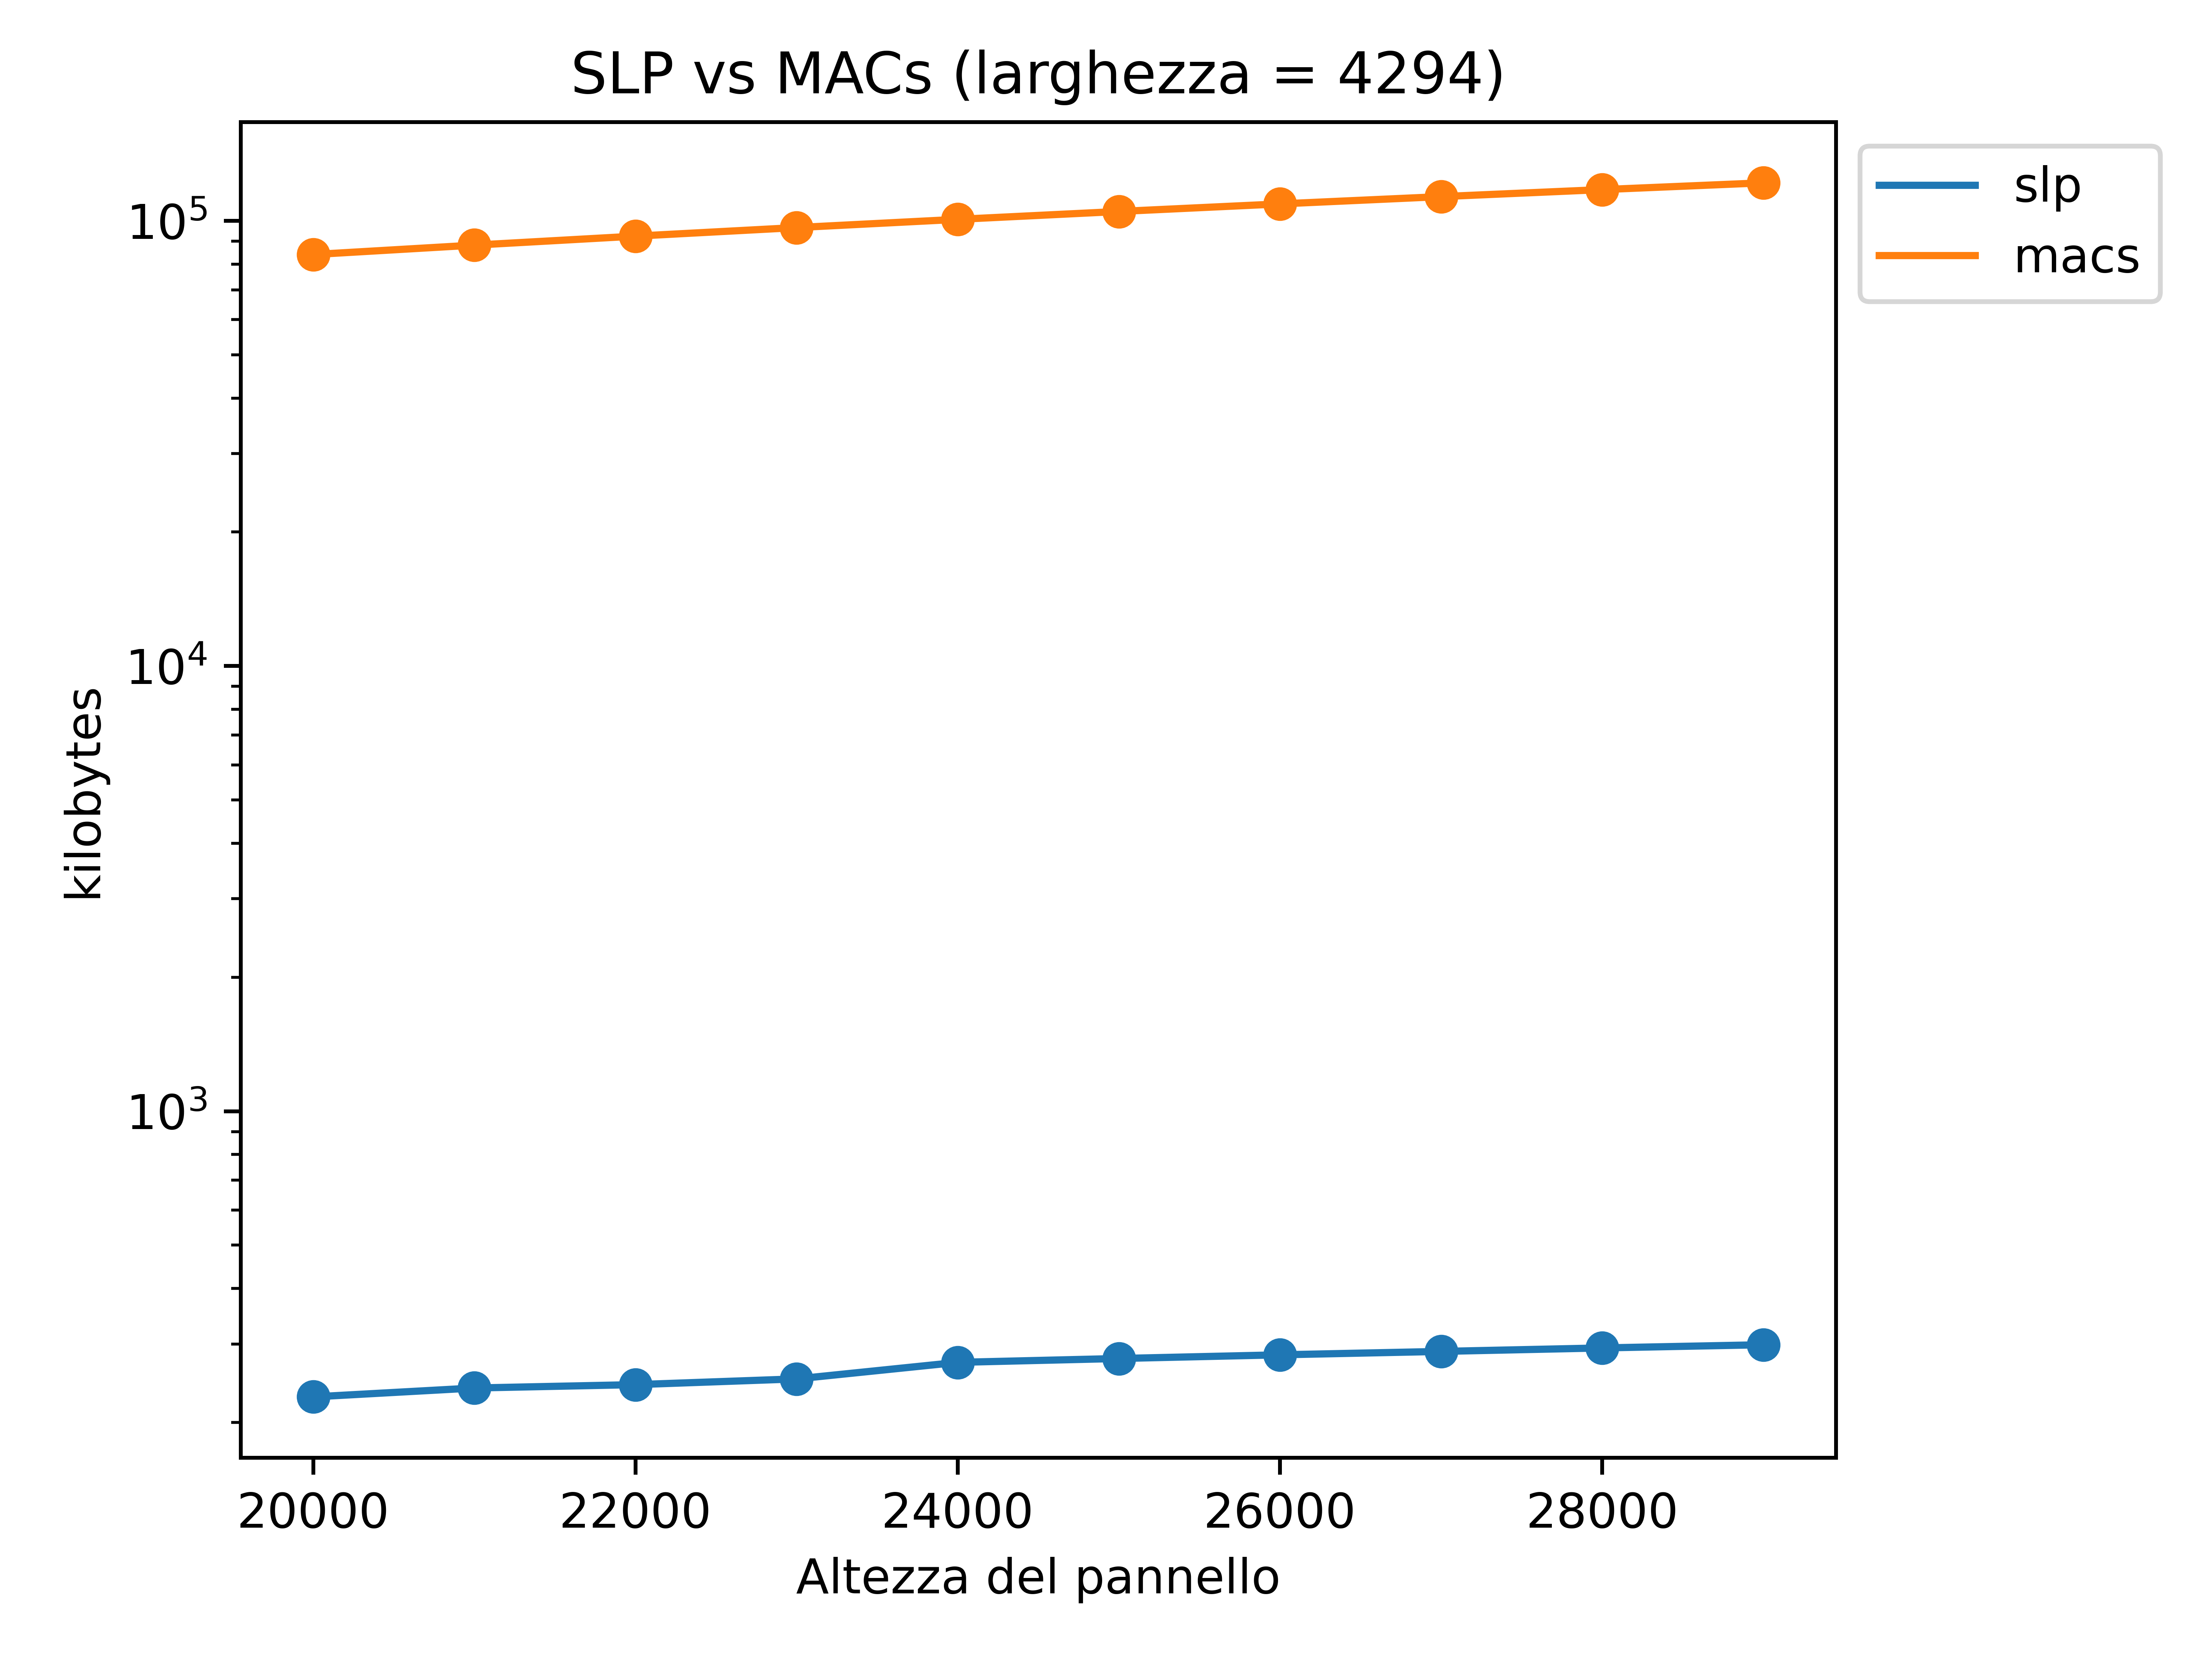
\includegraphics[scale = 0.6]{img/slp_vs_macs0.png}
  \caption{Confronto delle dimensioni, espresse in kilobytes, dei pannelli in
    formato \texttt{macs} e dei rispettivi \textit{SLP}. Il grafico è in scala
    logaritmica.}
  \label{fig:slpres1}
\end{figure}
Andando a vedere pannelli molto più grossi si nota come il rateo di
compressione continui essere proporzionale alla dimensione del pannello e,
nonostante il esso cresca di 
dimensione, la grandezza dell'\textit{SLP} resta molto piccola:
\begin{table}[H]
  \centering
  \begin{tabular}{c|c|c|c|c}
    \textbf{\#Samples} & \textbf{\#Siti} & \textbf{SLP (\textit{kb})}
    & \textbf{MACs (\textit{kb})} & \textbf{\%}\\
    \hline
    100000 & 358653 & 14771.0 & 35042963.54 & 0.0422\\
    100000 & 100000 & 9077.88 & 9075120.49 & 0.1\\
    100000 & 46538 & 8017.09 & 4448994.19 & 0.1802\\
  \end{tabular}
\end{table}
Tale risultato è anche apprezzabile in figura \ref{fig:slpres2}.
\begin{figure}
  \centering
  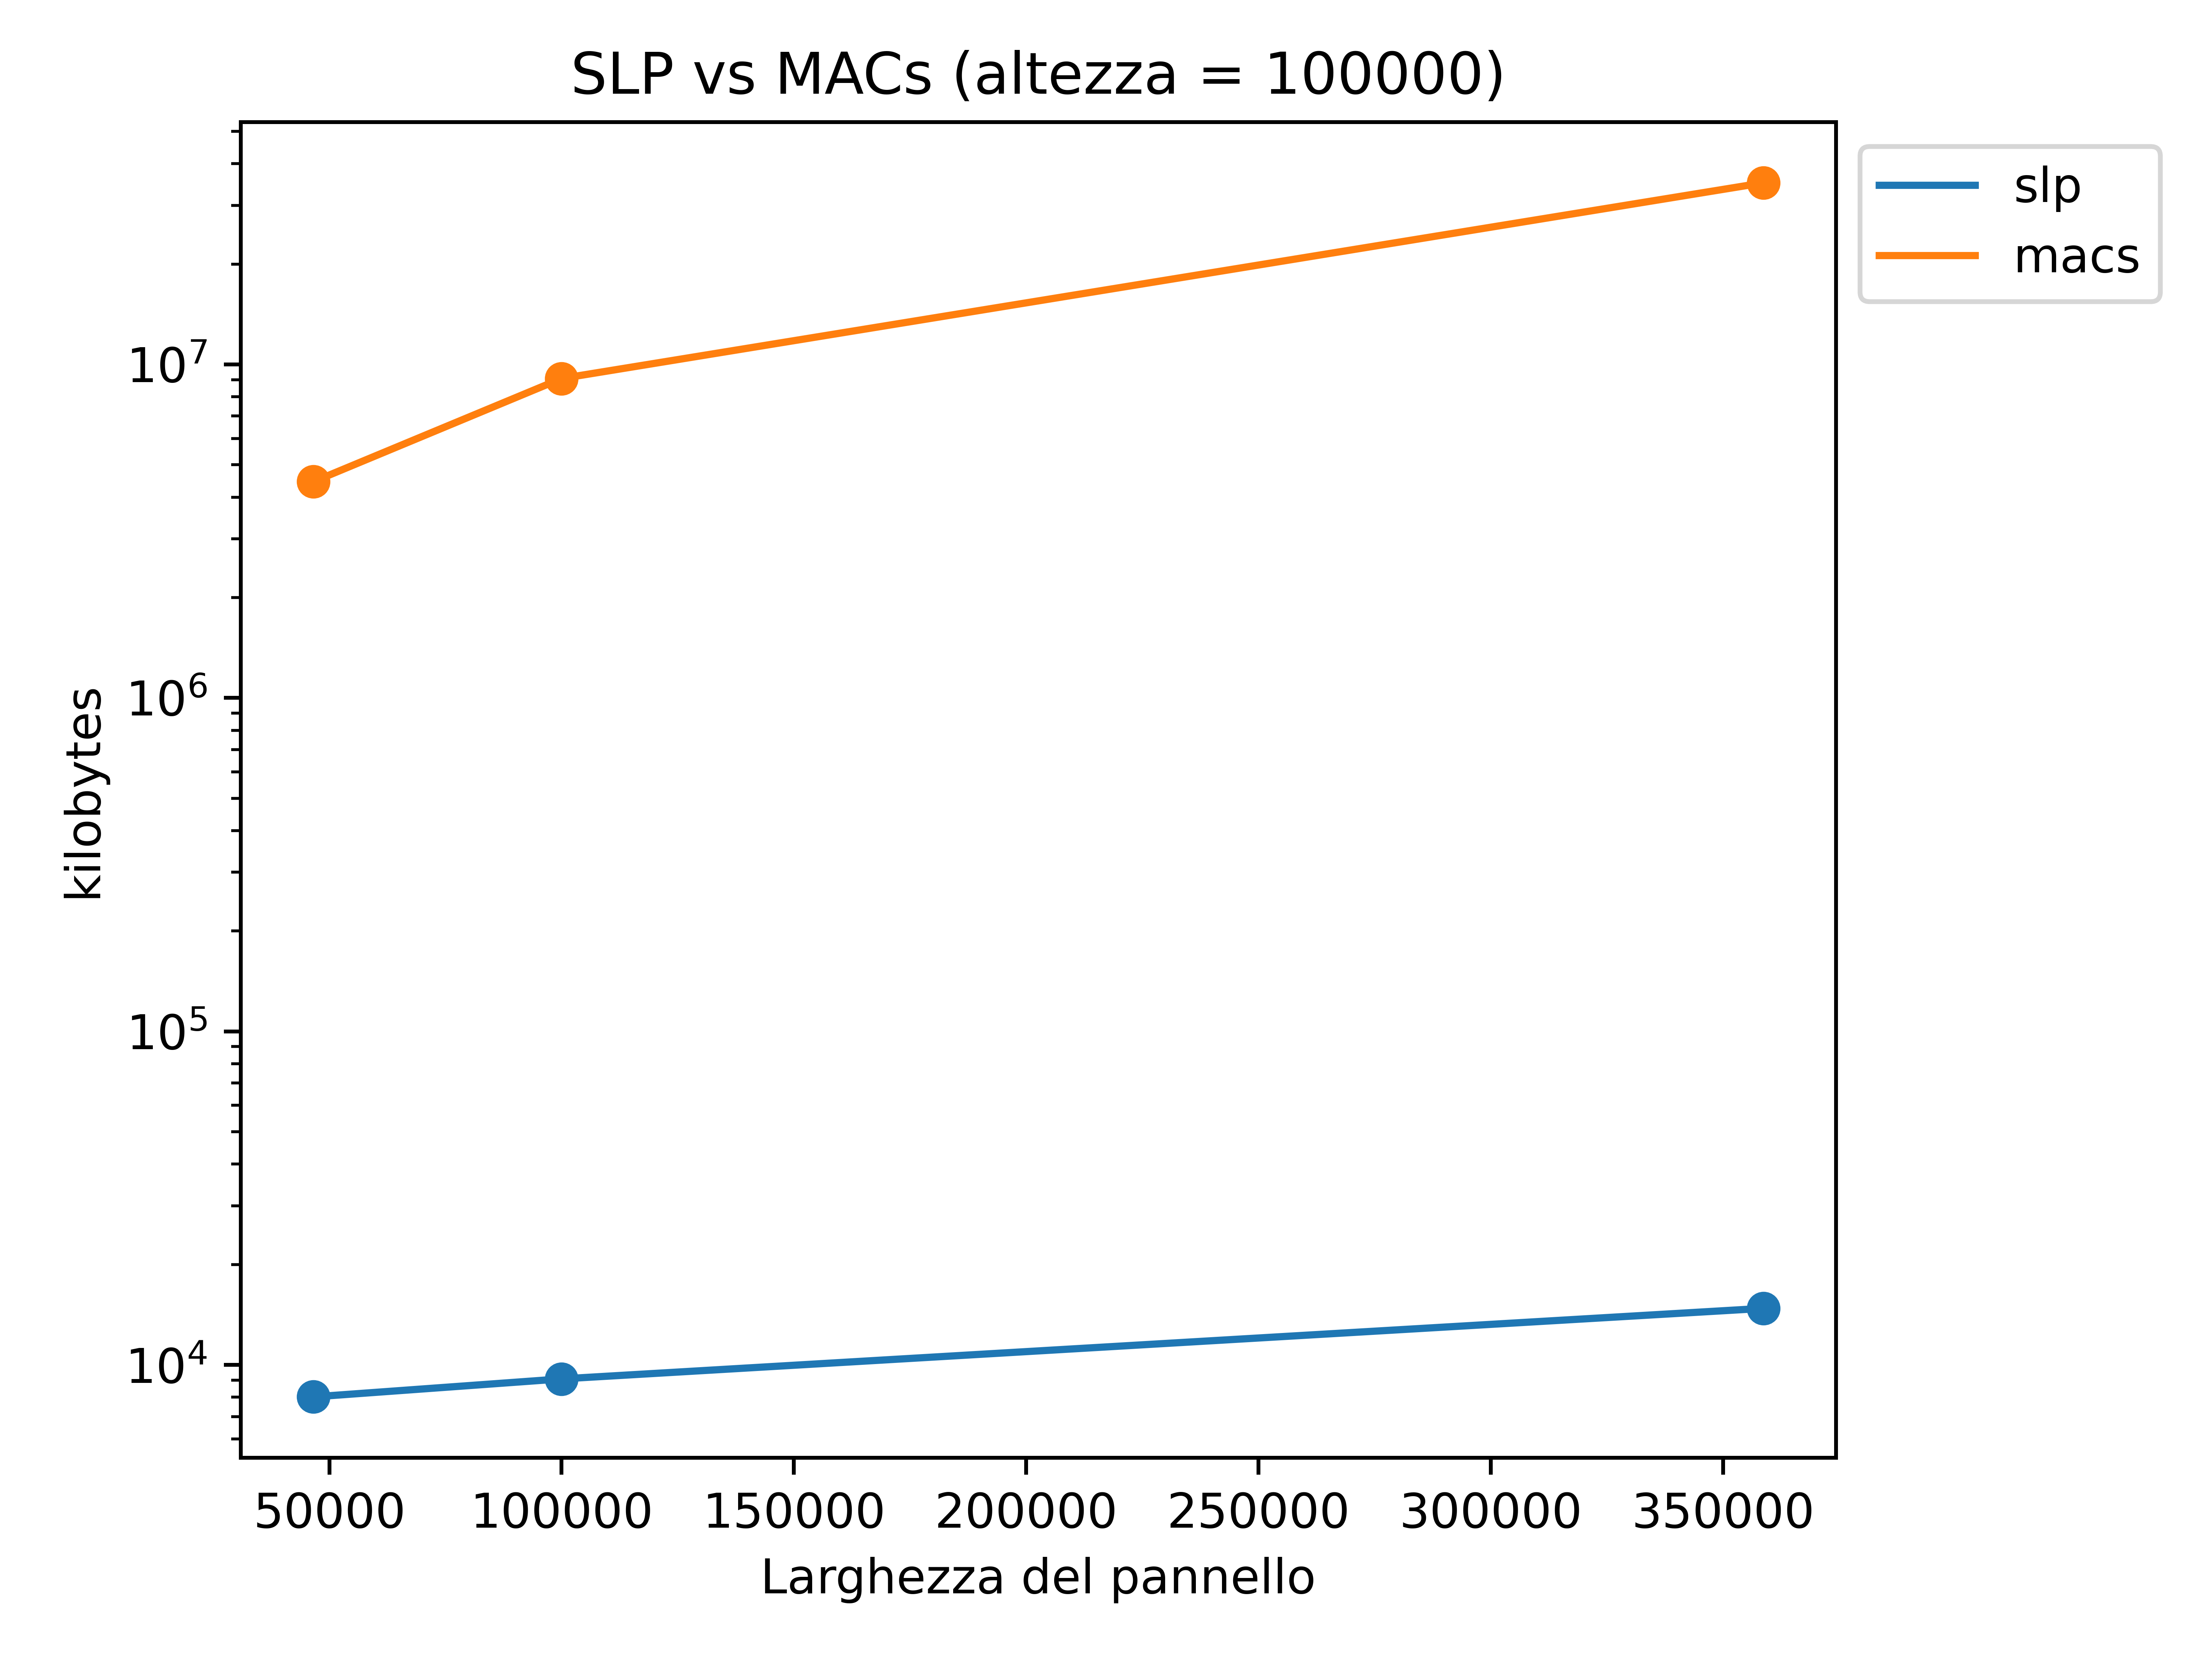
\includegraphics[scale = 0.6]{img/slp_vs_macs2.png}
  \caption{Confronto delle dimensioni, espresse in kilobytes, dei pannelli in
    formato \texttt{macs} e dei rispettivi \textit{SLP}. Il grafico è in scala
    logaritmica.}
  \label{fig:slpres2}
\end{figure}
Il caso estremo, un pannello $100000\times 358653$, occupante in memoria
circa 35gb in formato \texttt{.macs}, viene compresso in circa 15mb. Questo
accade soprattutto in quanto un pannello di soli simboli $\Sigma=\{0,1\}$
contiene molte ripetizioni, permettendo la costruzione di una grammatica,
tramite l'\textit{SLP}, particolarmente ``compatta''.\\
Si analizzano ora le due strutture dati, confrontando lo spazio richiesto dalle
varie sotto-strutture per effettuare il match con una query esterna, descritte
alle sezioni \ref{secpbwt}, \ref{secrlpbwtnaive}, \ref{secrlpbwtbv} e
\ref{secrlpbwtms}.\\
Si precisa che i dati ora descritti sono stati calcolati nel seguente modo:
\begin{itemize}
  \item per quanto riguarda la \textbf{PBWT}, sfruttando le stime fatte da
  Durbin stesso
  \item per quanto riguarda la \textbf{RLPBWT}, sfruttando le serializzazioni
  ottenute tramite \textit{SDSL}
\end{itemize}
Con un studio al leggero variare del pannello si nota, graficamente in figura
\ref{memcomp1}, come quanto descritto precedentemente venga confermato. Le
informazioni richieste dall'algoritmo 5 di Durbin sono quelle che richiedono
maggior memoria mentre la variante della \textit{RLPBWT} basata su \textit{SLP}
e \textit{LCE query} risulta essere la soluzione migliore tra le varianti della
\textit{RLPBWT}. Bisogna però notare come la soluzione \textit{matchDynamic}
ritrovabile nella repository della \textit{PBWT} risulti essere incredibilmente
più efficace, avendo, secondo Durbin stesso, una richiesta in spazio
proporzionale a $\mathcal{O}(M+N)$. \\
Limitiamo però ora il confronto all'algoritmo 5 di Durbin, in quanto obbiettivo
della tesi. Da un punto di vista di guadagno percentuale in memoria i risultati
sembrano essere interessanti, confrontando tale soluzione con la migliore per la
\textit{RLPBWT}:
\begin{table}[H]
  \centering
  \footnotesize
  \begin{tabular}{c|c|c|c|c}
    \textbf{\#Samples} & \textbf{\#Siti}
    & \textbf{RLPBWT SLP-LCE (\textit{kb})}
    & \textbf{PBWT Indexed (\textit{kb})} & \textbf{\%}\\
    \hline
    20000 & 4294 & 12118.62 & 1090270.65 & 1.1115\\
    21000 & 4294 & 12583.13 & 1144784.18 & 1.0992\\
    22000 & 4294 & 13033.78 & 1199297.71 & 1.0868\\
    23000 & 4294 & 13487.57 & 1253811.24 & 1.0757\\
    24000 & 4294 & 13954.44 & 1308324.78 & 1.0666\\
    25000 & 4294 & 14419.27 & 1362838.31 & 1.058\\
    26000 & 4294 & 14867.82 & 1417351.84 & 1.049\\
    27000 & 4294 & 15316.41 & 1471865.37 & 1.0406\\
    28000 & 4294 & 15765.41 & 1526378.9 & 1.0329\\
    29000 & 4294 & 16214.09 & 1580892.44 & 1.0256\\
  \end{tabular}
\end{table}
Provando in modo quantitativo l'efficacia in memoria della soluzione ultima
proposta in questa tesi.

% \begin{table}[H]
%   \centering
%   \tiny
%   \begin{tabular}{c|c|c|c|c|c|c|c|c}
%     \textbf{#Samples} & \textbf{#Siti} & \textbf{Na\"{I}Ve}
%     & \textbf{Bitvector} & \textbf{Pannello}
%     & \textbf{SLP-Thr} & \textbf{SLP-LCE} & \textbf{Indexed}&
%                                                               \textbf{Dynamic}\\
%     \hline
%     20000 & 4294 & 116872.34 & 118842.8 & 22956.56 & 12422.86 & 12118.62
%                                                      & 1090270.65 & 20004.19\\
%     21000 & 4294 & 122717.92 & 124689.87 & 23954.83 & 12884.39 & 12583.13
%                                                        & 1144784.18 & 21004.19\\
%     22000 & 4294 & 128541.43 & 130509.84 & 24911.04 & 13337.4 & 13033.78
%                                                        & 1199297.71 & 22004.19\\
%     23000 & 4294 & 134383.15 & 136347.63 & 25900.01 & 13789.62 & 13487.57
%                                                        & 1253811.24 & 23004.19\\
%     24000 & 4294 & 140197.73 & 142157.96 & 26853.09 & 14239.5 & 13954.44
%                                                        & 1308324.78 & 24004.19\\
%     25000 & 4294 & 146047.34 & 148014.12 & 27855.43 & 14705.09 & 14419.27
%                                                        & 1362838.31 & 25004.19\\
%     26000 & 4294 & 151872.56 & 153834.89 & 28841.15 & 15154.06 & 14867.82
%                                                        & 1417351.84 & 26004.19\\
%     27000 & 4294 & 157711.32 & 159670.04 & 29793.47 & 15603.17 & 15316.41
%                                                        & 1471865.37 & 27004.19\\
%     28000 & 4294 & 163536.4 & 165489.58 & 30779.6 & 16052.56 & 15765.41
%                                                        & 1526378.9 & 28004.19\\
%     29000 & 4294 & 169381.28 & 171331.14 & 31765.37 & 16501.58 & 16214.09
%                                                        & 1580892.44 & 29004.19\\
    
%   \end{tabular}
% \end{table}
\begin{figure}
  \centering
  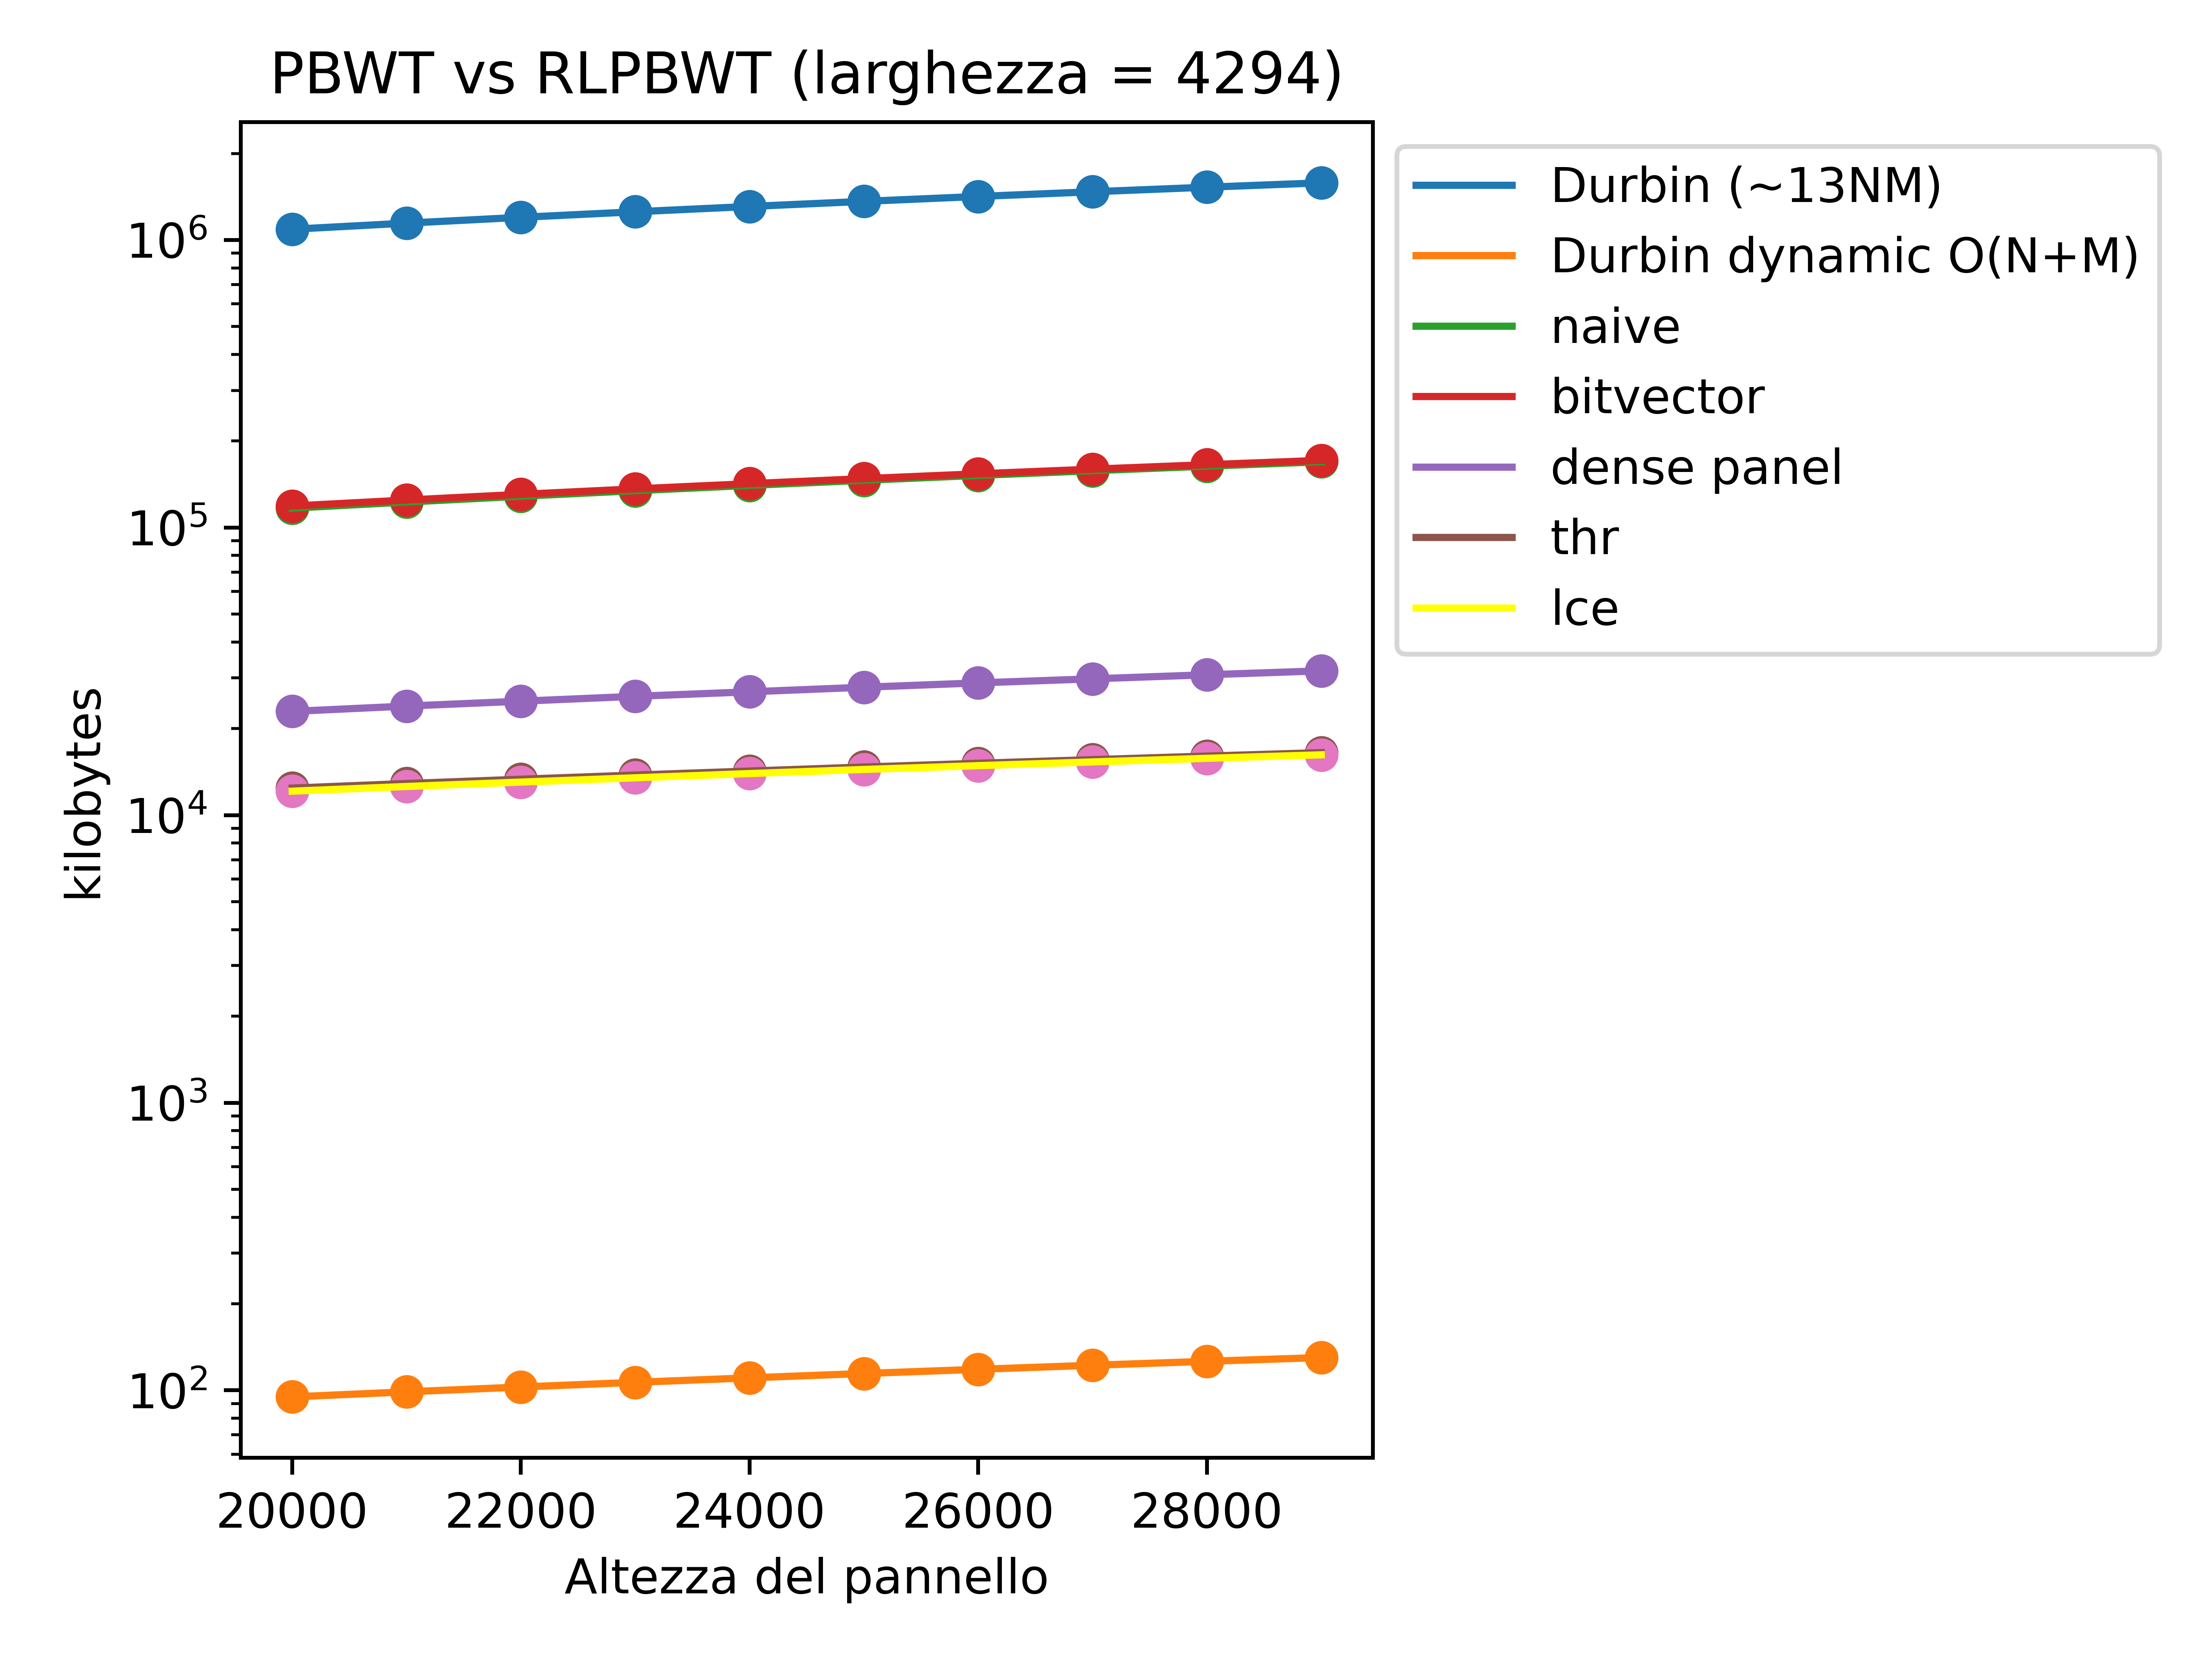
\includegraphics[scale = 0.6]{img/pbwt_vs_rlpbwt_dyn.png}
  \caption{Confronto dello spazio in memoria, in kilobytes, richiesto dalle
    varie strutture dati.} 
  \label{memcomp1}
\end{figure}
\paragraph{Tempi di esecuzione}
Bisogna infine considerare i tempi di esecuzione per il pattern matching con un
pannello di query. Dal punto di vista della \textit{RLPBWT} bisogna considerare
in primis due aspetti:
\begin{itemize}
  \item avere meno informazione in memoria comporta molto probabilmente, a
  parità di risultati, tempi maggiori
  \item l'uso di strutture dati succinte ed eventualmente dell'\textit{SLP}
  comporta costi dal punto di vista temporale. Come anticipato in sezione
  \ref{bvsec}, le operazioni sugli sparse bitvector non sono tutte i tempo
  costante e, come invece anticipato in sezione \ref{slpsec}, gli \textit{SLP}
  non garantiscono \textit{random access} in tempo costante e questo, per quanto
  poi l'algoritmo di estensione sia efficiente, si ripercuote anche sul calcolo
  delle \textit{LCE query}
\end{itemize}
Questa premessa fa capire come ci si aspettasse che i tempi fossero maggiori con
la \textit{RLPBWT}, in ogni sua variante, rispetto all'algoritmo 5 di Durbin.
Parlando invece dell'algoritmo \textit{matchDynamic} si ha che, per quanto
asintoticamente presenti la stessa complessità dell'algoritmo 5, ovvero
$\mathcal{O}(N(M+Q))$, con $Q$ numero di query, esso risulta incredibilmente più
performante. \\
Alcuni risultati sono visualizzabili in figura \ref{fig:1000} e \ref{fig:10000},
dove si possono osservare sia i tempi che lo spazio richiesto. Anche la completa
esecuzione quindi conferma come l'algoritmo 5 sia incredibilmente esoso dal
punto di vista dello spazio richiesto, pur avendo ottime performance
temporali. Dal punto di vista invece delle varianti della \textit{RLPBWT} si
nota come:
\begin{itemize}
  \item la \textit{RLPBWT na\"{i}ve}, priva dell'uso dei bitvector e
  dell'\textit{SLP}, risulti essere la più performante, anche se, si ricordi,
  non permette di identificare quali righe stiano effettivamente matchando ma
  solo quante
  \item la \textit{RLPBWT con bitvector}, avente lo stesso limite della variante
  na\"{i}ve, presenta anche maggiori costi in termini di memoria di quest'ultima,
  avendo anch'essa ancora l'\textit{LCP array} completo ma anche tutte le
  informazioni memorizzate in bitvector, che aumentano, come anticipato, i tempi
  di calcolo. La chiave delle varianti che sfruttano
  le \textit{matching statistics} è infatti quella di non avere l'\textit{array
    LCP} in memoria, una delle cause principali dell'aumento di spazio richiesto
  \item le tre varianti basate sulle \textit{matching statistics} hanno spazio
  occupato pressoché uguale, anche se si può percepire, nei due casi studiati,
  come il tenere l'intero pannello in forma di bitvector, all'aumentare della
  grandezza dello stesso, comporti molta più memoria degli \textit{SLP}. Dal
  punto di vista temporale, inoltre, anche se si ha \textit{random access} in
  tempo costante, all'aumentare del pannello, il numero di accessi allo stesso
  comporta forti costi in termini di tempo macchina. Questi
  ultimi, infatti, come già visto occupano pochissima memoria anche con pannelli
  molto estesi. Dal punto di vista temporale si rileva come la variante basata
  su \textit{SLP} e \textit{threshold} richieda molto più tempo. Si nota che ciò
  accade a causa di due fattori:
  \begin{itemize}
    \item il continuo accesso all'\textit{SLP} per calcolare $MS[i].len$
    \item l'eventuale accesso all'\textit{SLP} per disambiguare le threshold a
    fine run
  \end{itemize}
  Tra le tre quindi la variante con \textit{SLP} e \textit{LCE query},
  all'aumentare della grandezza del pannello, risulta essere la soluzione
  migliore
\end{itemize}

\begin{figure}
  \centering
  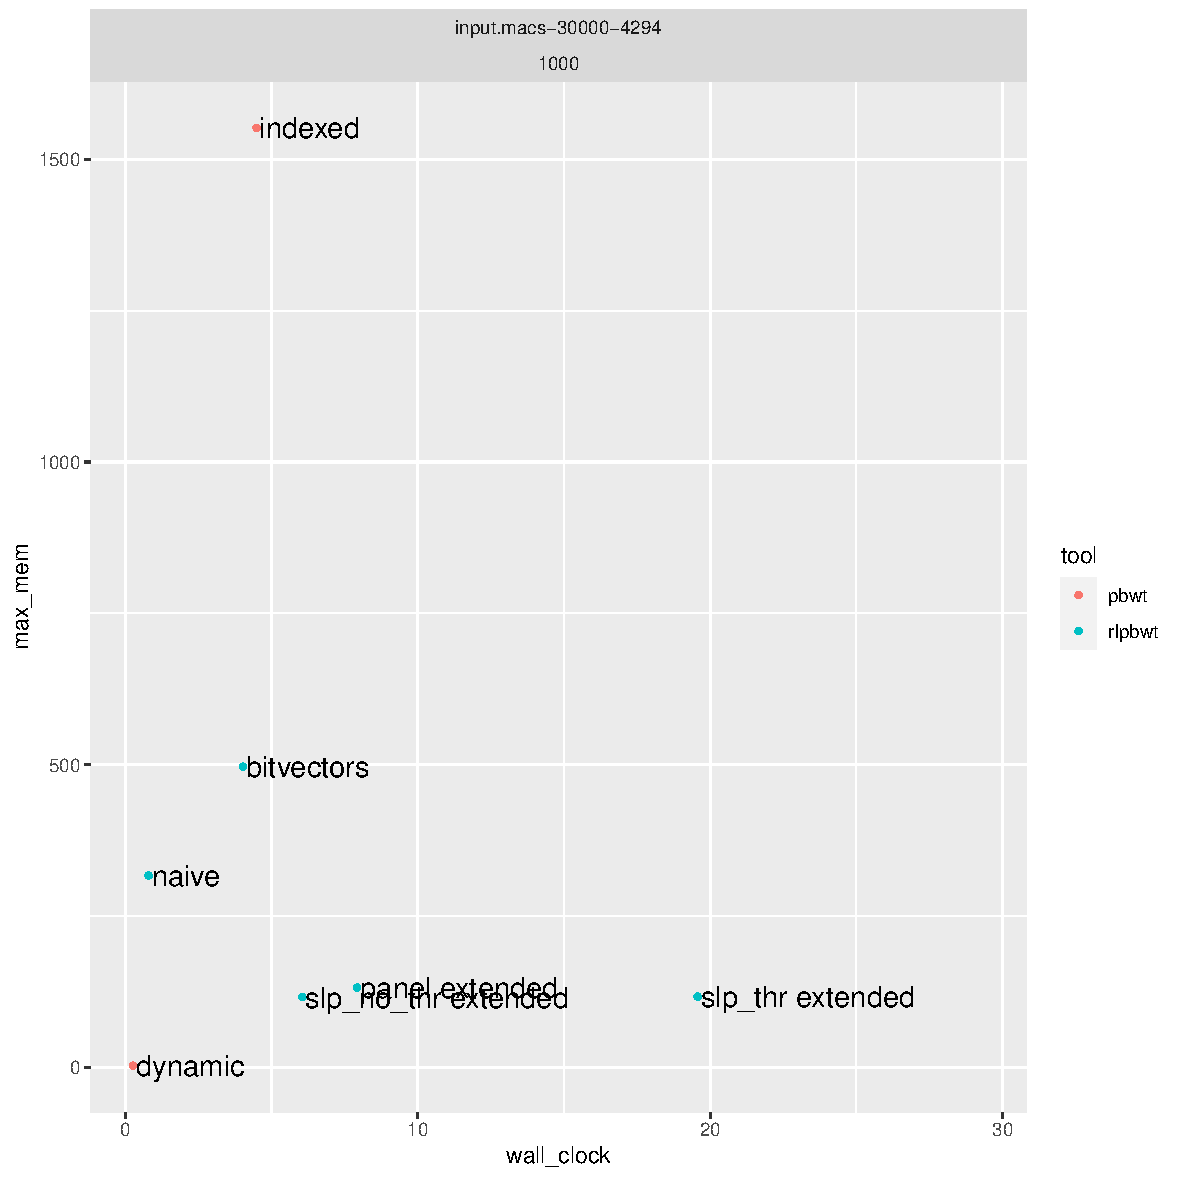
\includegraphics[scale = 0.35]{img/time_vs_mem_1000.pdf}
  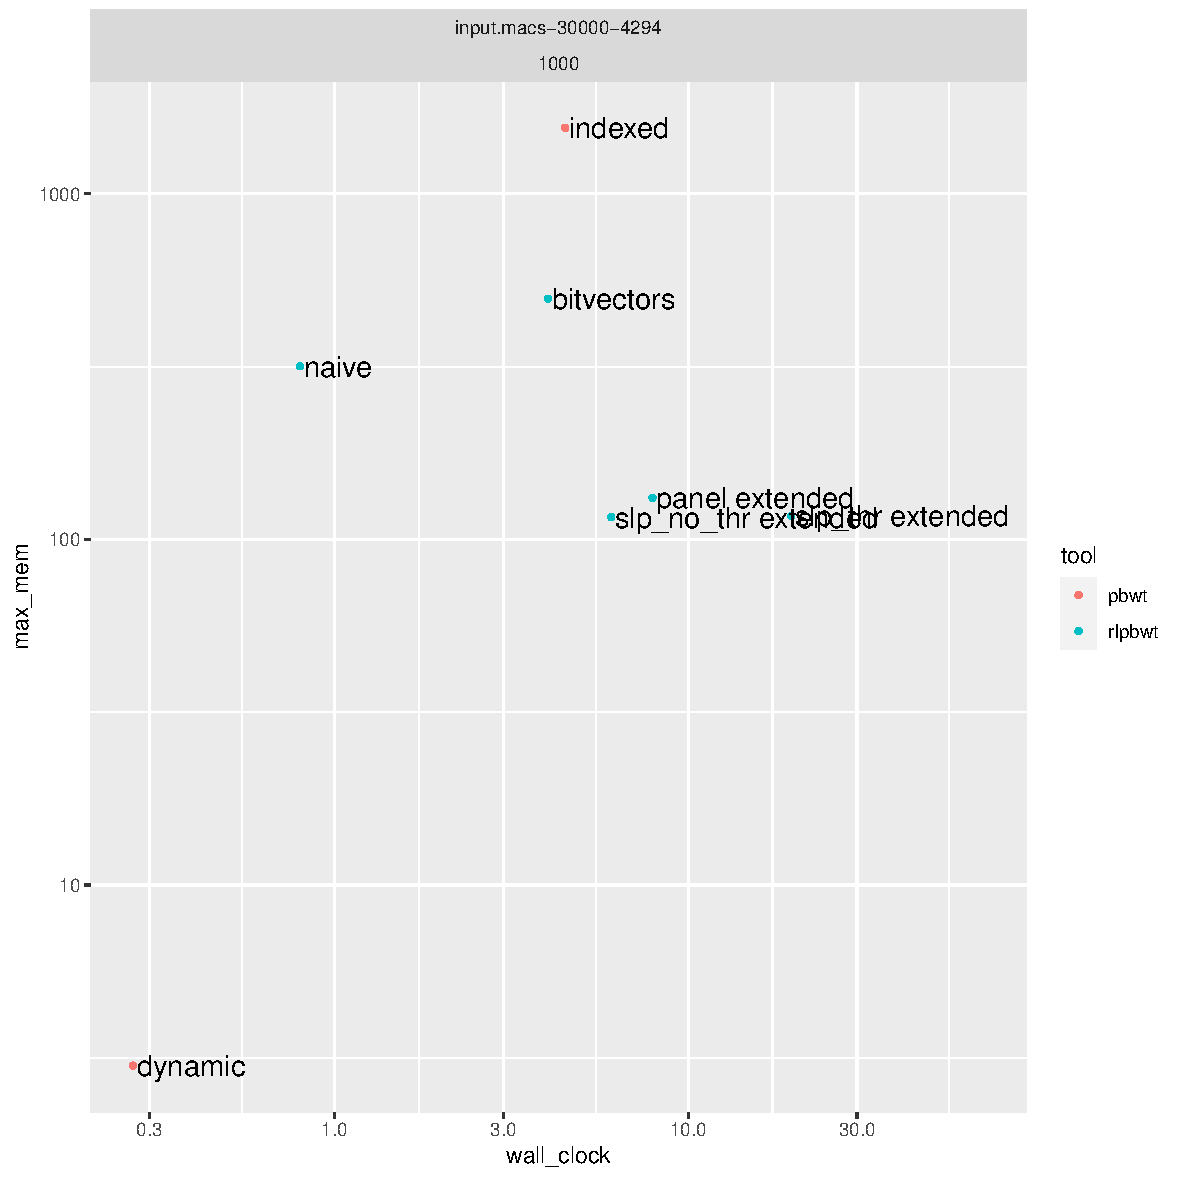
\includegraphics[scale = 0.35]{img/time_vs_mem-loglog_1000.pdf}
  \caption{Esecuzione dei vari algoritmi di match su un pannello
    $29000\times 4294$ e 1000 query.  Il grafico a destra è in scala
    logaritmica. }
  \label{fig:1000}
\end{figure}

\begin{figure}
  \centering
  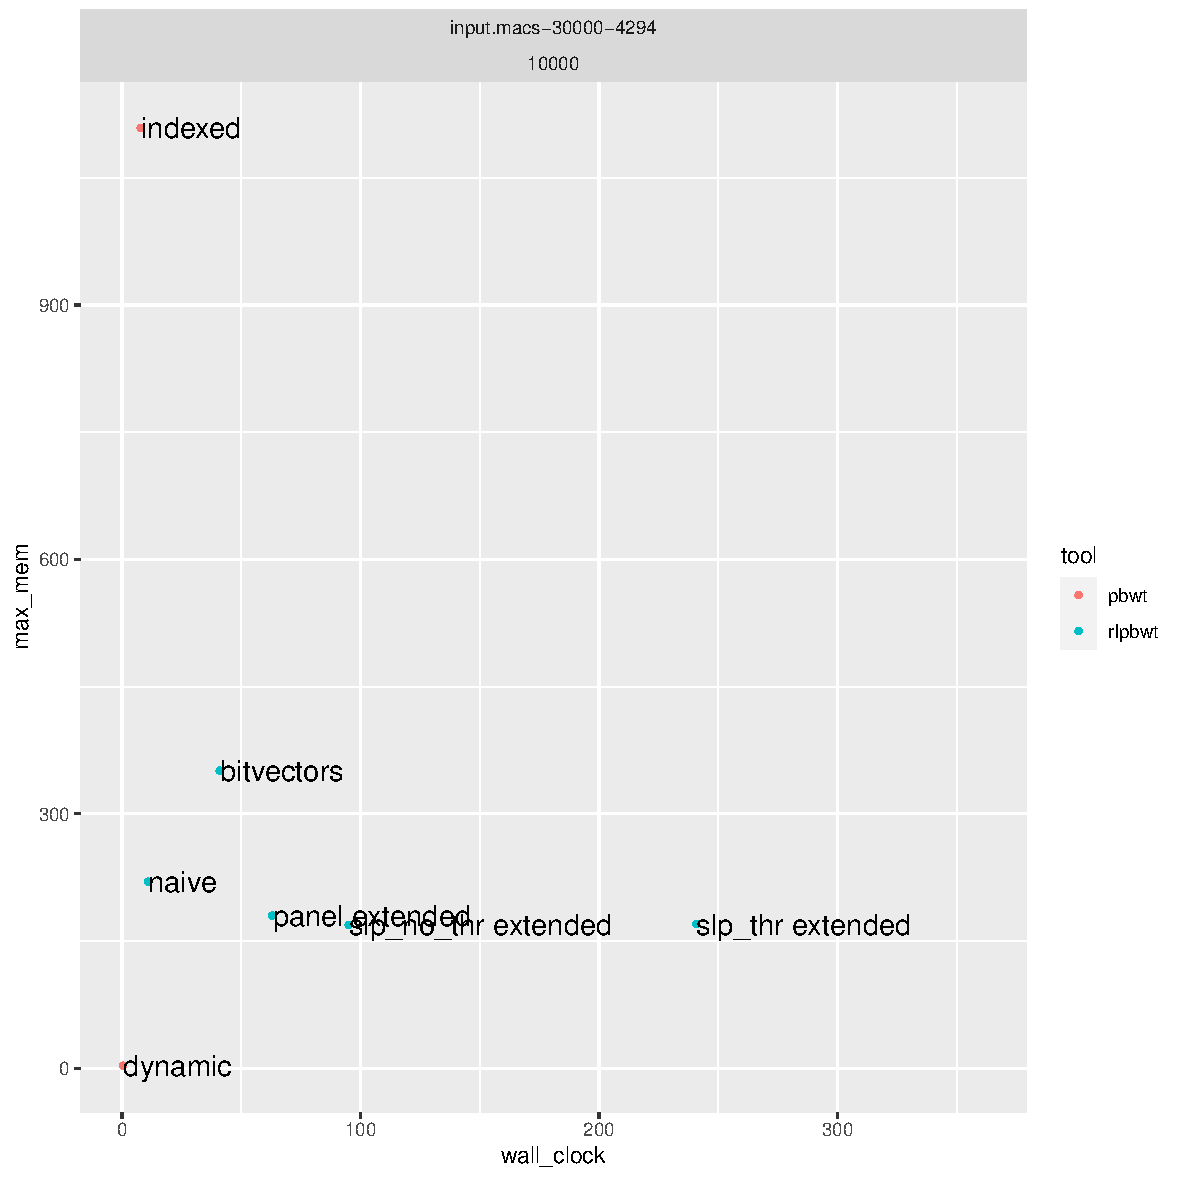
\includegraphics[scale = 0.35]{img/time_vs_mem_10000.pdf}
  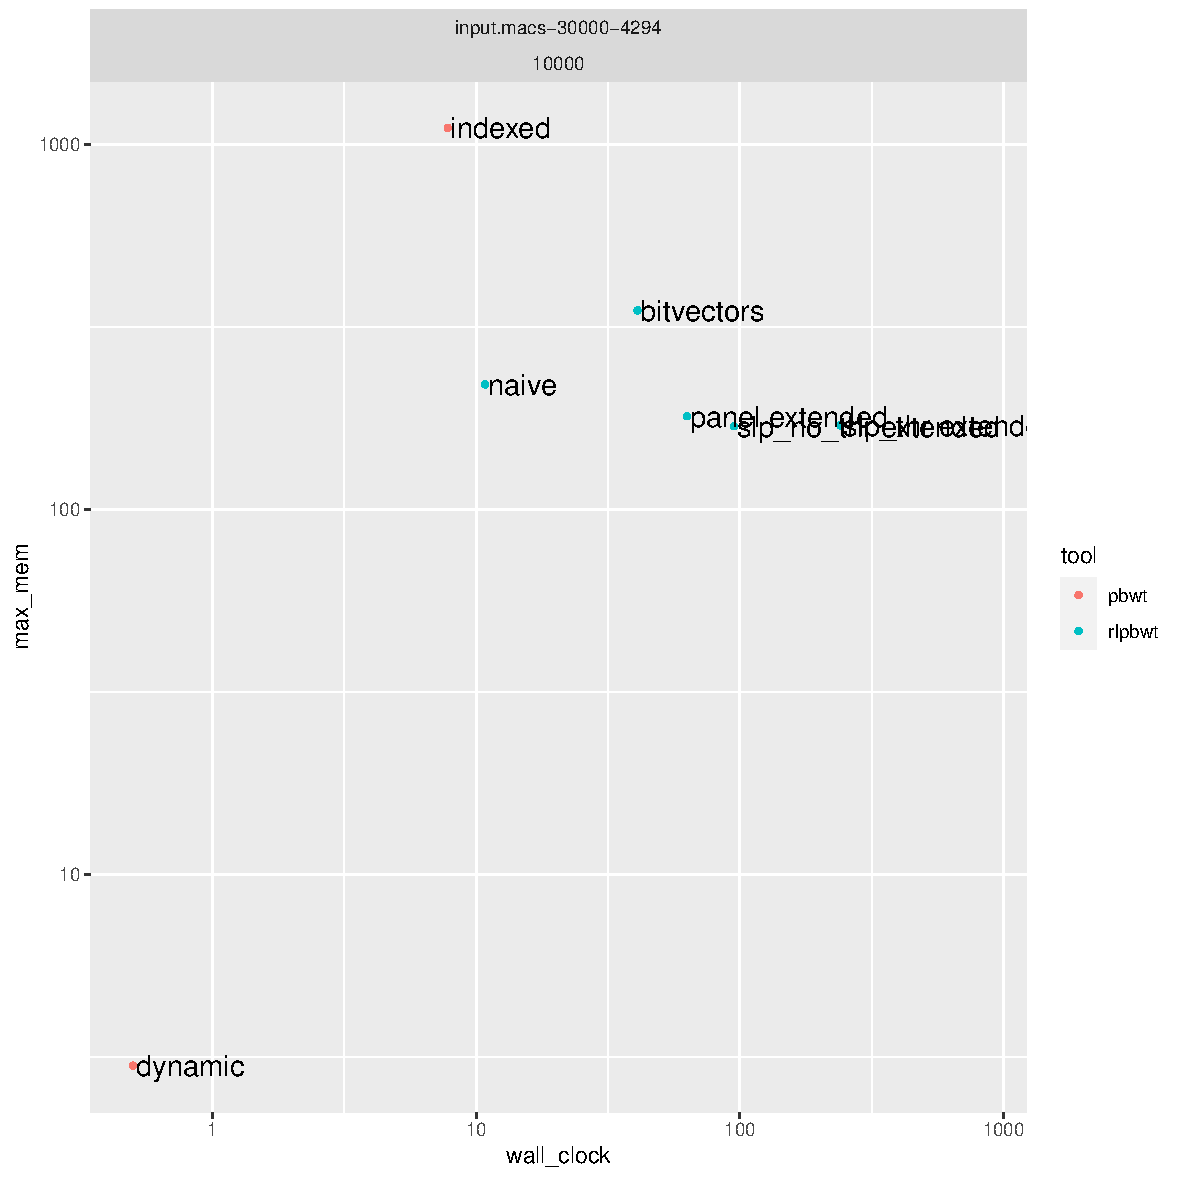
\includegraphics[scale = 0.35]{img/time_vs_mem-loglog_10000.pdf}
  \caption{Esecuzione dei vari algoritmi di match su un pannello
    $20000\times 4294$ e 10000 query. Il grafico a destra è in scala
    logaritmica. }
  \label{fig:10000}
\end{figure}
Per completezza, in figura \ref{fig:bigres}, si riportano anche i risultati in
tempo 
e spazio di una sperimentazione su un pannello di grandi dimensioni:
$70000\times 46538$ con $30000$ query. Sono riportati anche i risultati delle
tre varianti basate su \textit{matching statistics} senza l'estensione dei match
tramite le \textbf{funzioni} $\boldsymbol \varphi$ e
$\boldsymbol\varphi^{\mathbf{-1}}$. Si può notare come la struttura dati aggiuntiva
non comporti praticamente alcuna differenza sostanziale sia in termini di
memoria che di tempo di calcolo. In merito agli altri risultati si ha che
seguono tutti il trend già descritto negli esempi precedenti. In particolare si
nota che:
\begin{itemize}
  \item l'algoritmo 5 di Durbin ha una richiesta di memoria davvero molto
  grande, parlando di circa 40.75 gb di memoria richiesta
  \item l'algoritmo \textit{matchDynamic} di Durbin risulta essere migliore sia
  dal punto di vista dello spazio richiesto che del tempo d'esecuzione. Parlando
  di tempi, infatti, l'intera esecuzione richiede $\sim 22$s, contro i $\sim
  411$ dell'algoritmo \textit{matchIndexed} e i $\sim 1824$ della
  \textit{RLPBWT} con \textit{SLP} e \textit{LCE query}
  \item la variante \textit{RLPBWT} con \textit{SLP} e \textit{threshold}, per
  le problematiche già descritte richiede un tempo d'esecuzione importante,
  parlando di circa 2 ore di esecuzione
\end{itemize}
\begin{figure}
  \centering
  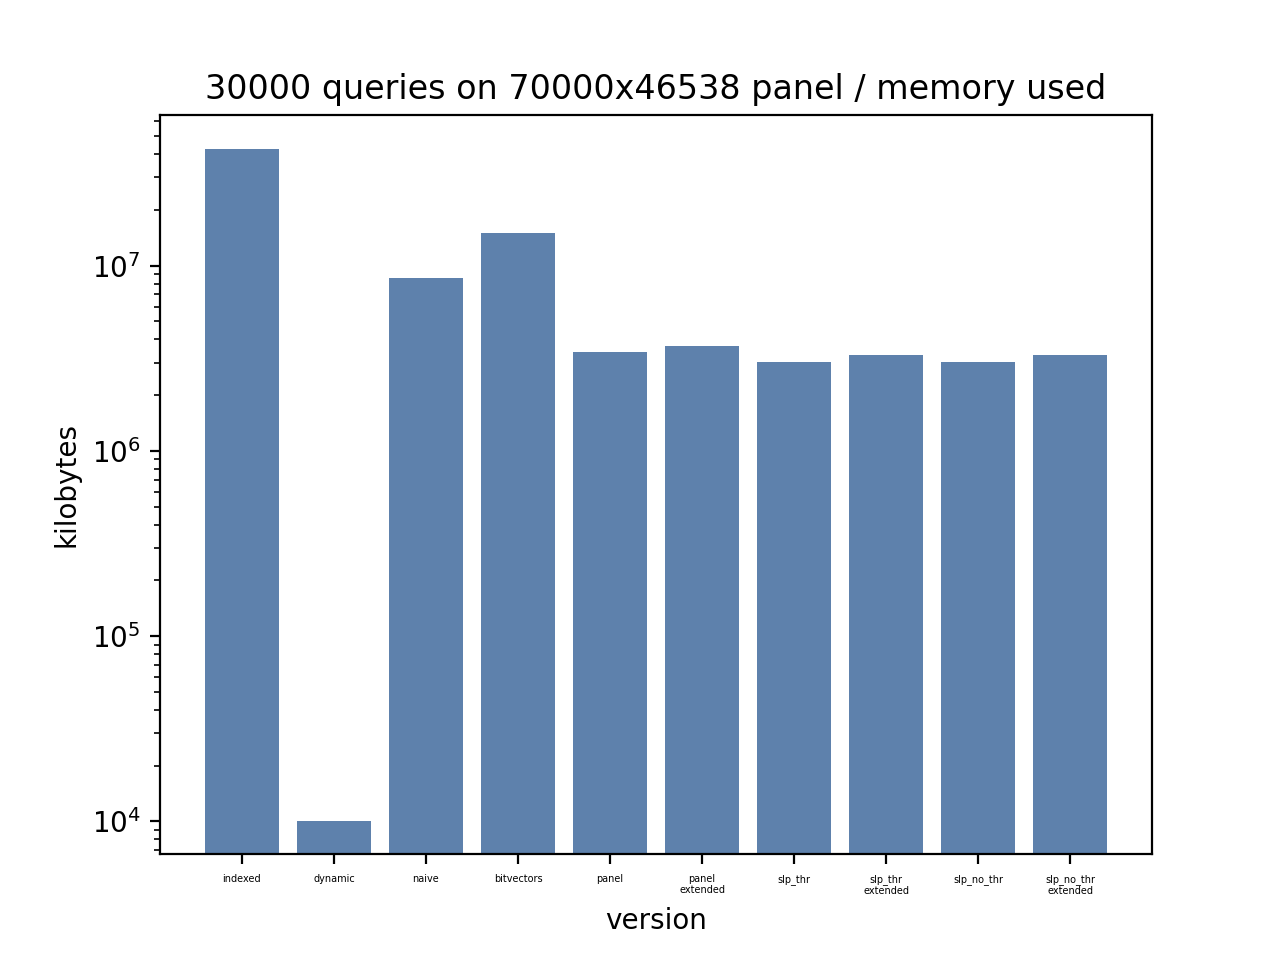
\includegraphics[scale = 0.4]{img/mem.png}
  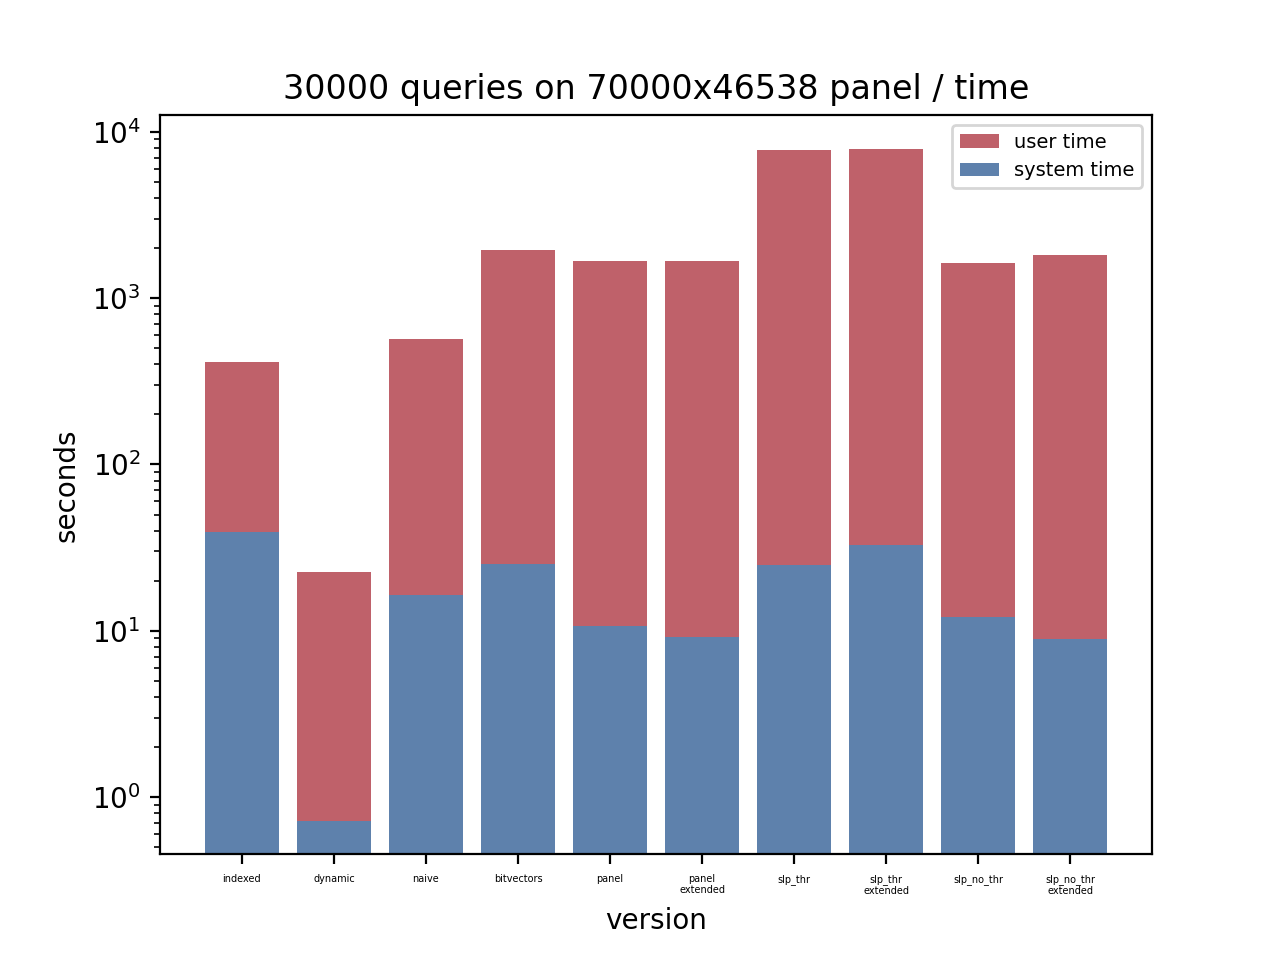
\includegraphics[scale = 0.4]{img/time.png}
  \caption{Risultati, in scala logaritmica, dell'esecuzione dei vari algoritmi
    su un pannello di grosse dimensioni. Si noti che, quantitativamente, la
    variante \textit{matchIndexed} richieda $42736132$ kb di memoria mentre la
    \textit{RLPBWT} con \textit{SLP} e \textit{LCE query} solo $3286424$ kb,
    richiedendo quindi appena il 7\% di memoria richiesta dall'algoritmo 5 di
    Durbin. Infine, per quanto la scala logaritmica renda impercettibile tale
    differenza, la variante \textit{RLPBWT} con pannello richiede $3695968$ kb,
    quindi circa $380$ mb in più della soluzione basata sull'uso
    dell'\textit{SLP}. } 
  \label{fig:bigres}
\end{figure}
\section{Sperimentazione sui pannelli reali}
Al fine di valorizzare maggiormente i risultati ottenuti in questo progetto, si
è deciso di procedere con lo studio di dati reali, relativi alla \textit{phase
  3} del \textbf{1000
  Genome
  Project}\footnote{\url{https://ftp.1000genomes.ebi.ac.uk/vol1/ftp/release/20130502/}}
\cite{1kgp}.\\ 
Tali pannelli, disponibili in formato \textit{VCF}, presentano un numero
costante di sample, ovvero 5008, mentre a variare è il numero di siti. Essendo
dati reali, non si ha la sola presenza di siti biallelici. Si è quindi proceduto
alla selezione dei soli siti biallelici, ottenendo quindi pannelli costruiti su
un alfabeto binario $\Sigma=\{0,1\}$, tramite l'uso di \textbf{bcftools}
\cite{bcftools}, tramite il comando \texttt{bcftools view -m2 -M2
  -v snps}.\\
La prima selezione dei pannelli è stata dettata dalla volontà di studiare, per
praticità, matrici non troppo estese. Si sono, quindi, scelti i pannelli
relativi:
\begin{itemize}
  \item al cromosoma 22, con 1055454 siti
  \item al cromosoma 20, con 1739315 siti
  \item al cromosoma 18, con 2171378 siti
  \item al cromosoma 16, con 2596072 siti
\end{itemize}
In aggiunta, si è studiato uno dei pannelli più grossi disponibili, ovvero
quello relativo al cromosoma 1, con 6196151 siti.\\
Al fine del computo degli SMEM, avendo un numero ridotto di sample a
disposizione, si è scelto di estrarre da ognuno 100 sample da usare come
query.\\
Prima di procedere con l'effettivo studio delle performance di calcolo degli
SMEM, trattandosi di pannelli reali, è risultata interessante una preliminare
indagine esplorativa sulla natura di tali pannelli in termini di
\textit{sparsità} degli alleli e di conseguente numerosità delle run. Si è
quindi calcolato, per i cinque pannelli, il numero di simboli $\sigma=0$ e
$\sigma=1$, notando come il numero di simboli $\sigma=1$ fosse molto ridotto
rispetto al totale, essendo il $\sim 0.03\%$ del totale dei simboli. Una tale
sparsità del dato si ``propaga'' anche sul numero di run di ogni colonna, avendo
di fatto pochi simboli $\sigma=1$ in ogni colonna, simboli che possono anche
essere nella medesima run dopo la permutazione data dalla
\textit{PBWT}. Si ricordi, inoltre, che tale permutazione. come per la
\textit{BWT}, è studiata per essere 
maggiormente efficiente nel caso del dato biologico. Studiando, quindi, il
numero medio di run per colonna e il numero 
massimo di run in una colonna si è confermato tale risultato, infatti:
\begin{itemize}
  \item per il cromosoma 22 si ha un numero medio di 14 run, con un massimo di
  2450
  \item per il cromosoma 20 si ha un numero medio di 11 run, con un massimo di
  2176
  \item per il cromosoma 18 si ha un numero medio di 11 run, con un massimo di
  2365
  \item per il cromosoma 16 si ha un numero medio di 12 run, con un massimo di
  2330
  \item per il cromosoma 1 si ha un numero medio di 11 run, con un massimo di
  2721 
\end{itemize}
Si conferma quindi il risultato atteso, risultato che è a favore, in termini di
complessità in spazio, della \textit{RLPBWT} in quanto tutte le componenti sono
proporzionali al numero di run. In figura \ref{fig:chrrun} si riportano
graficamente tali risultati.
\begin{figure}
  \centering
  \begin{subfigure}{.45\textwidth}
    \centering
    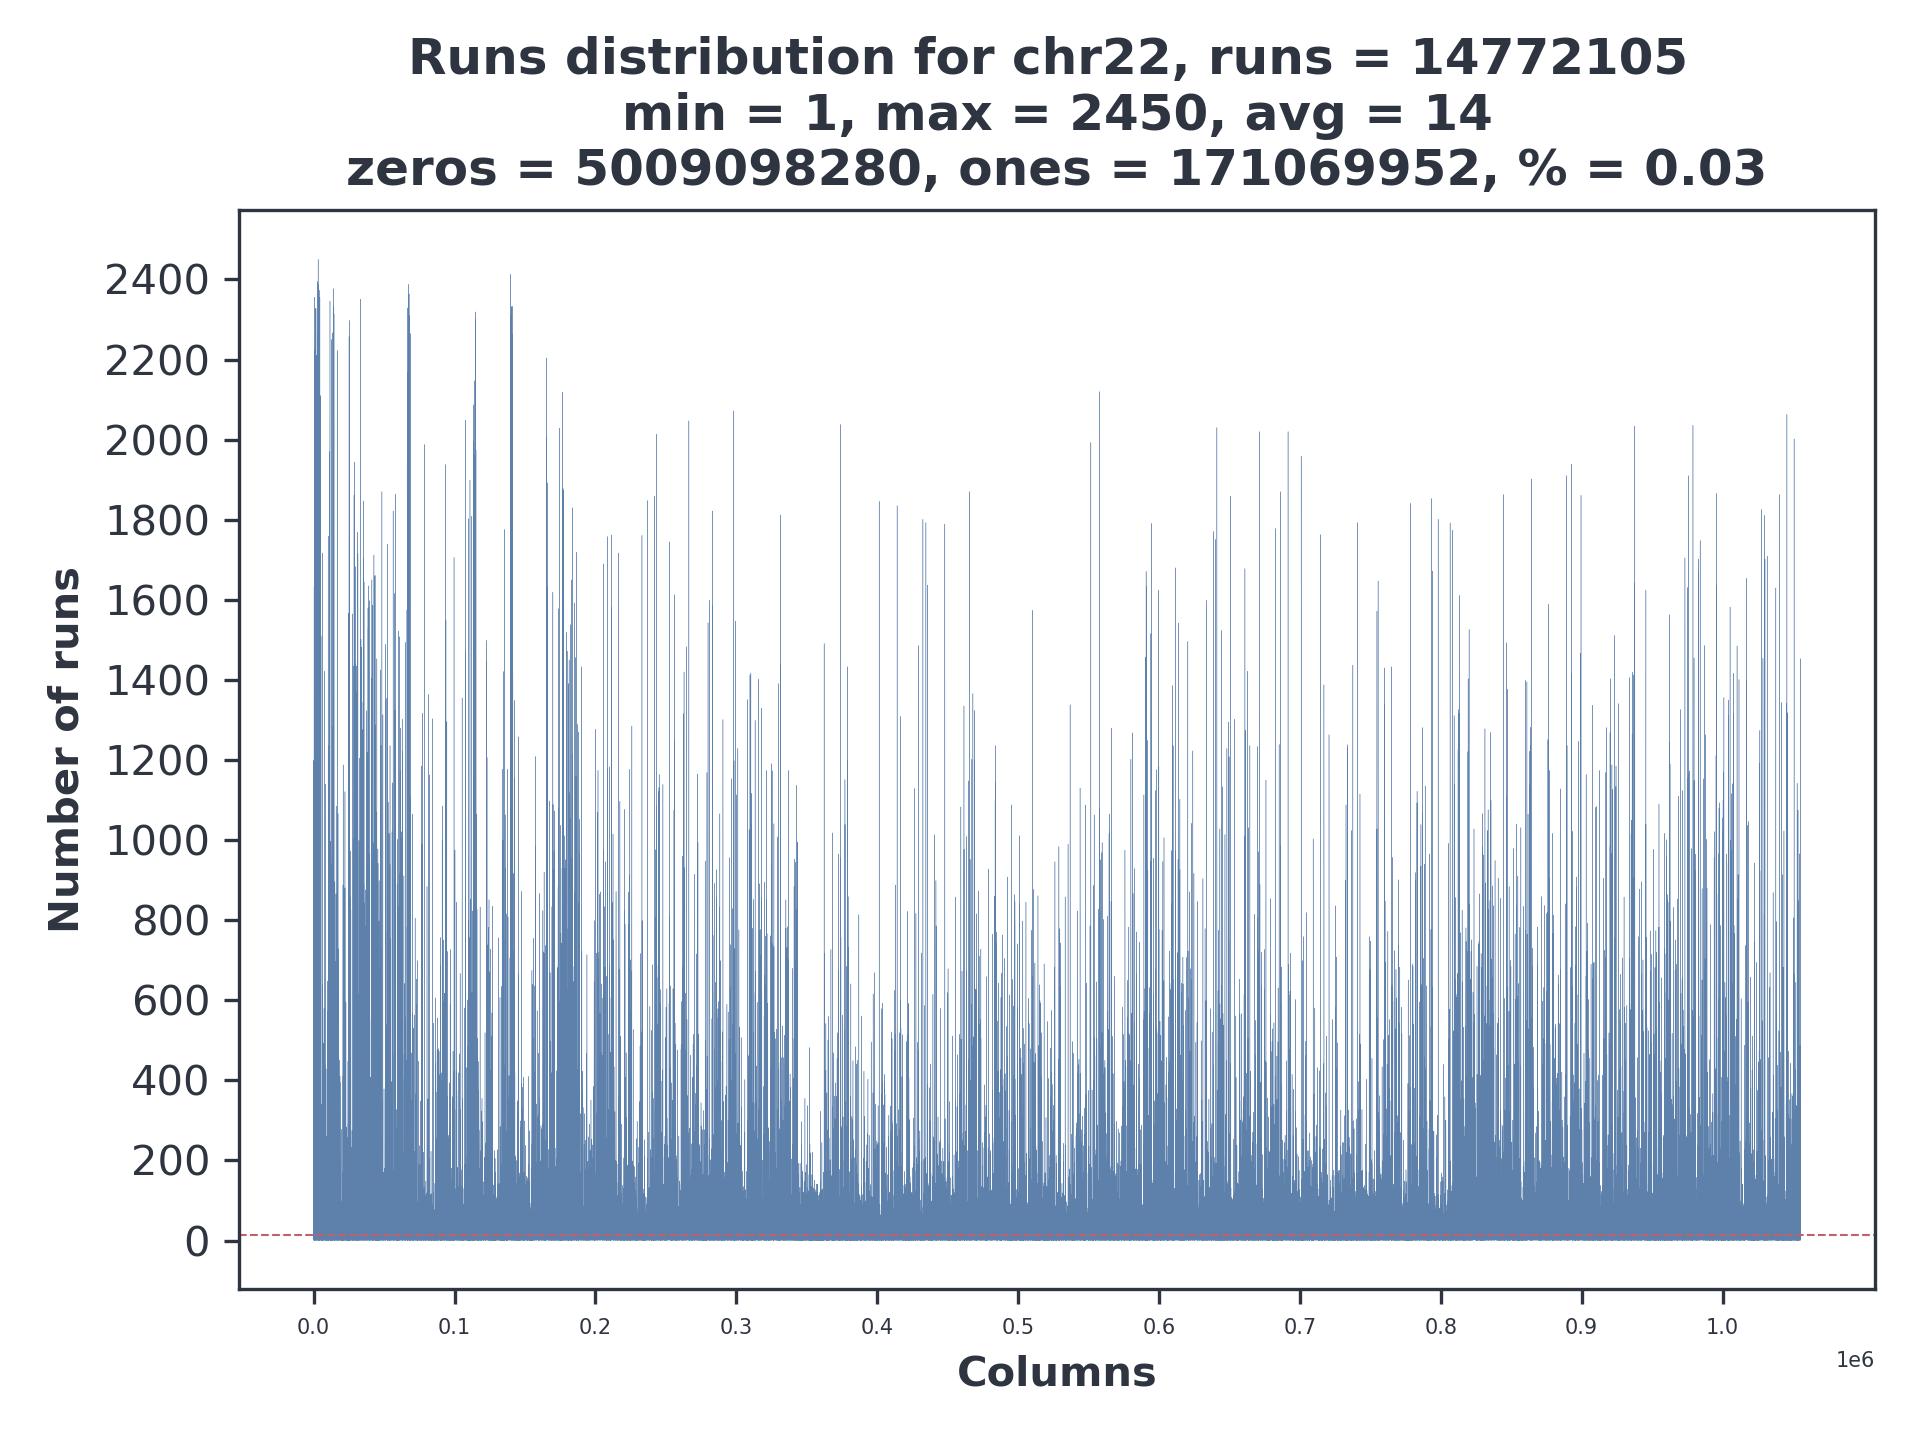
\includegraphics[width=\linewidth]{img/22_runs.png}
  \end{subfigure}%
  \begin{subfigure}{.45\textwidth}
    \centering
    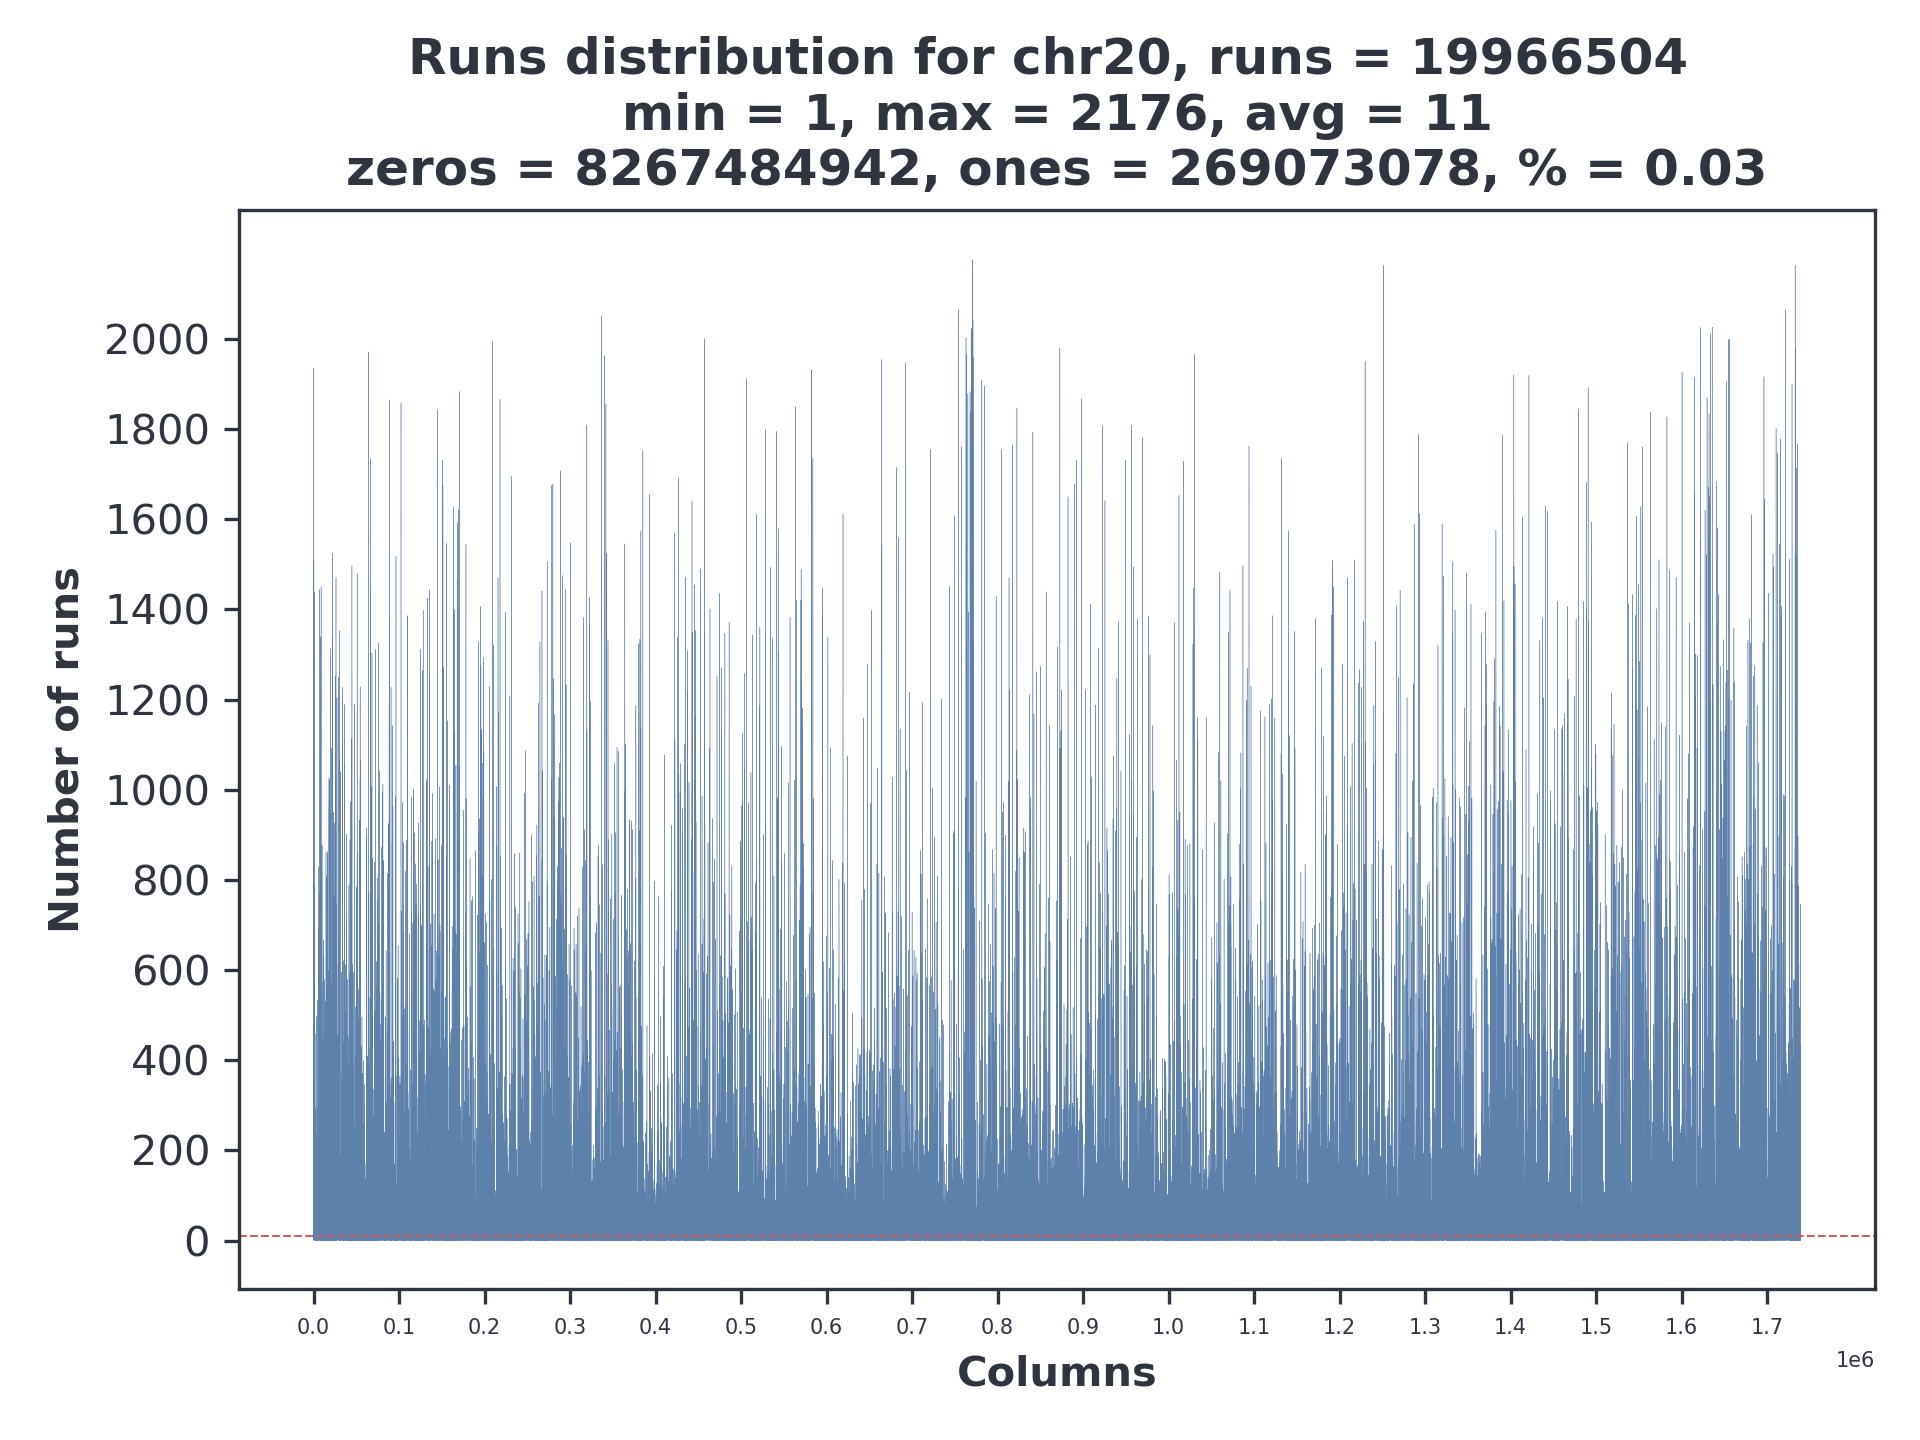
\includegraphics[width=\linewidth]{img/20_runs.png}
  \end{subfigure}
  \begin{subfigure}{.45\textwidth}
    \centering
    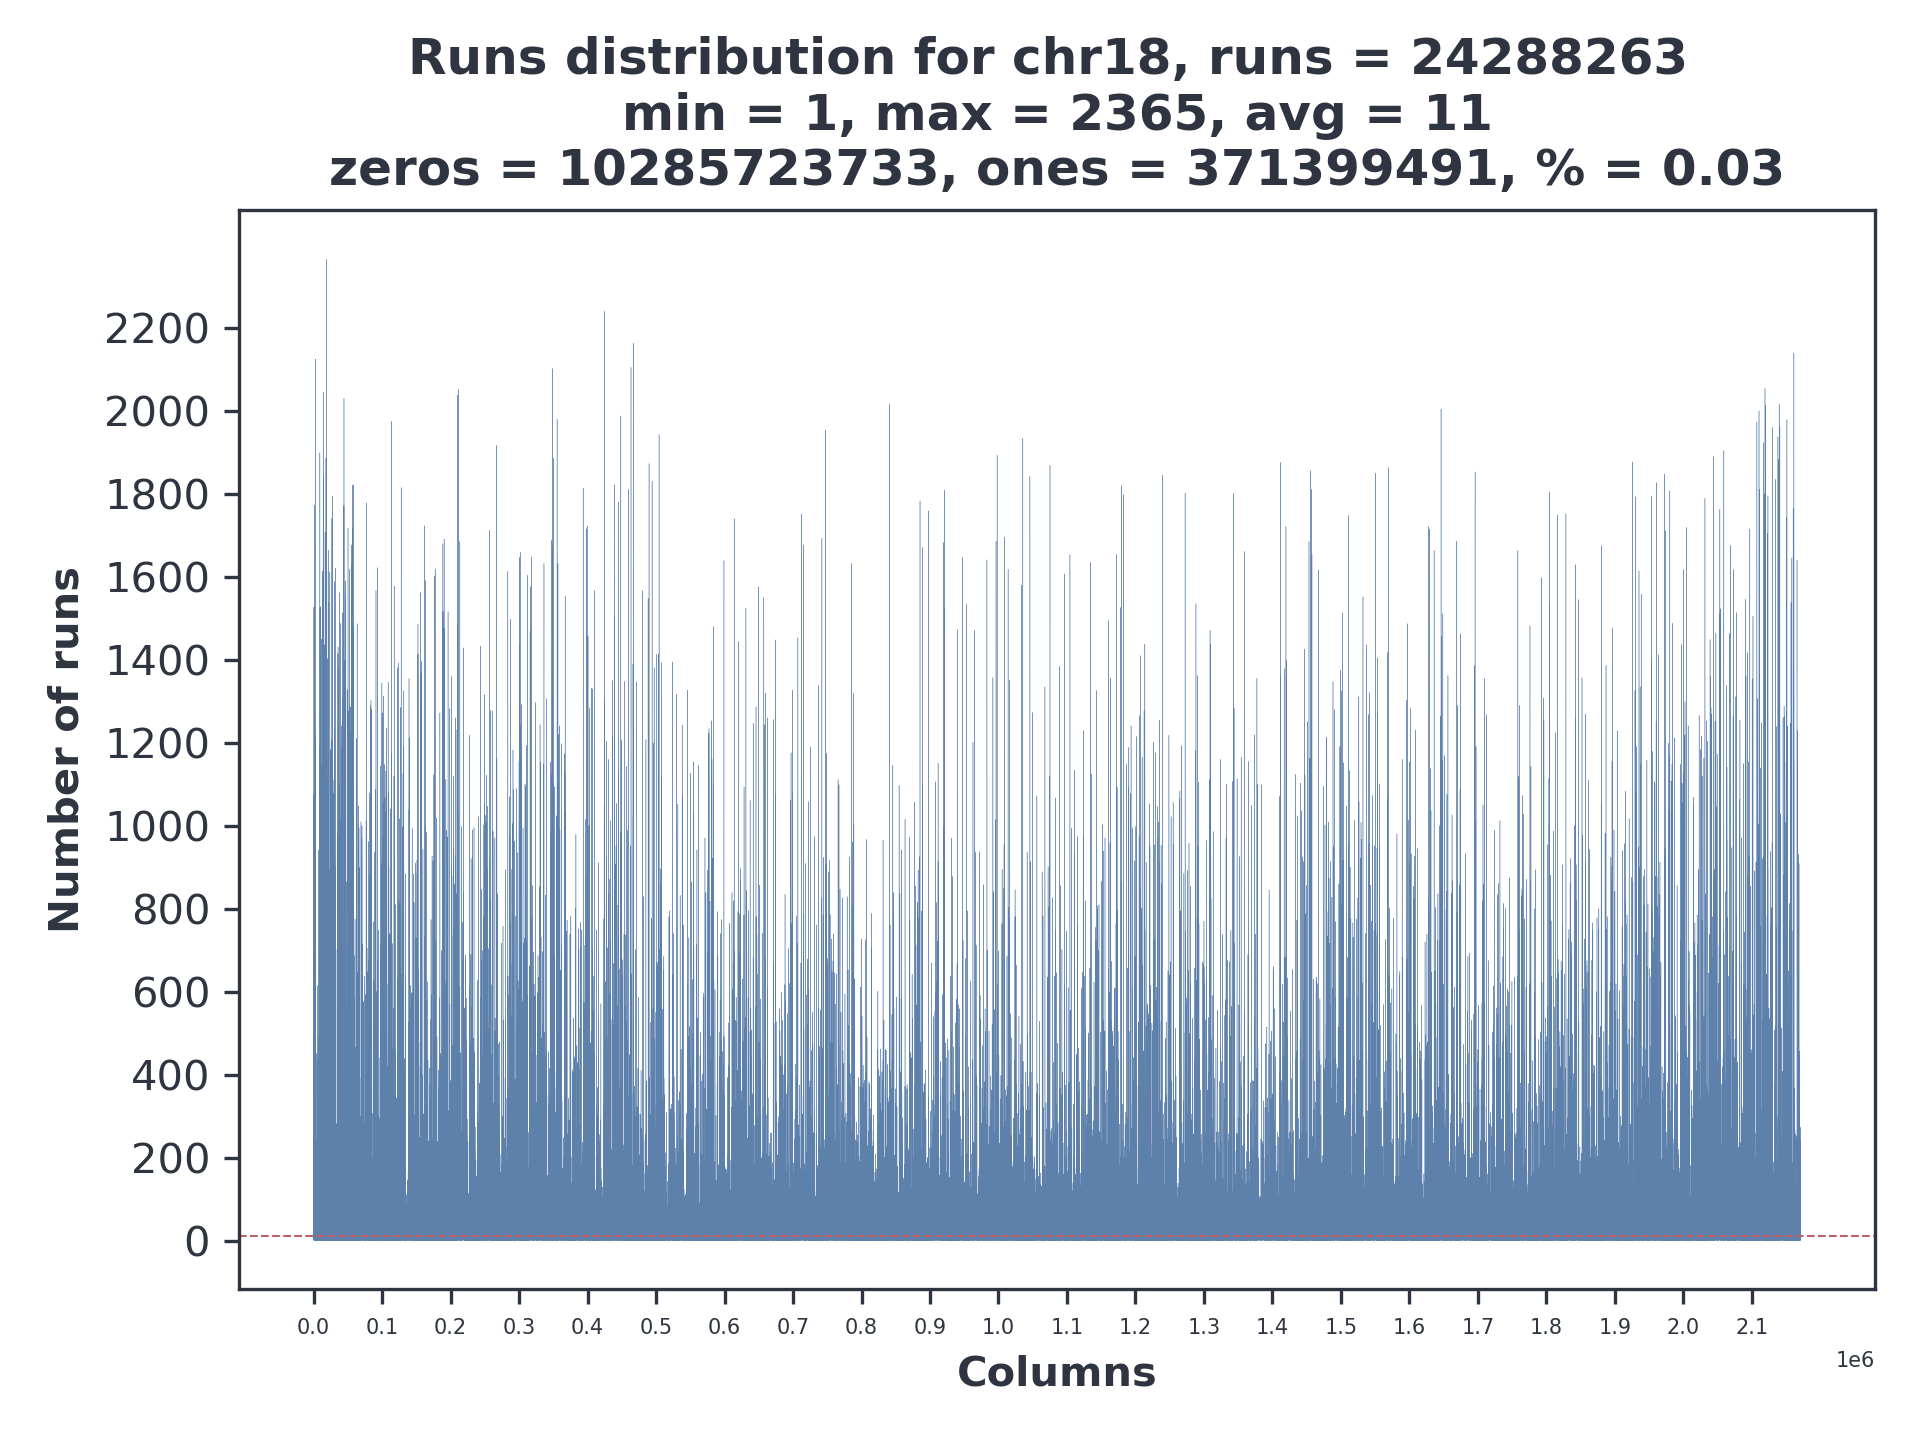
\includegraphics[width=\linewidth]{img/18_runs.png}
  \end{subfigure}%
  \begin{subfigure}{.45\textwidth}
    \centering
    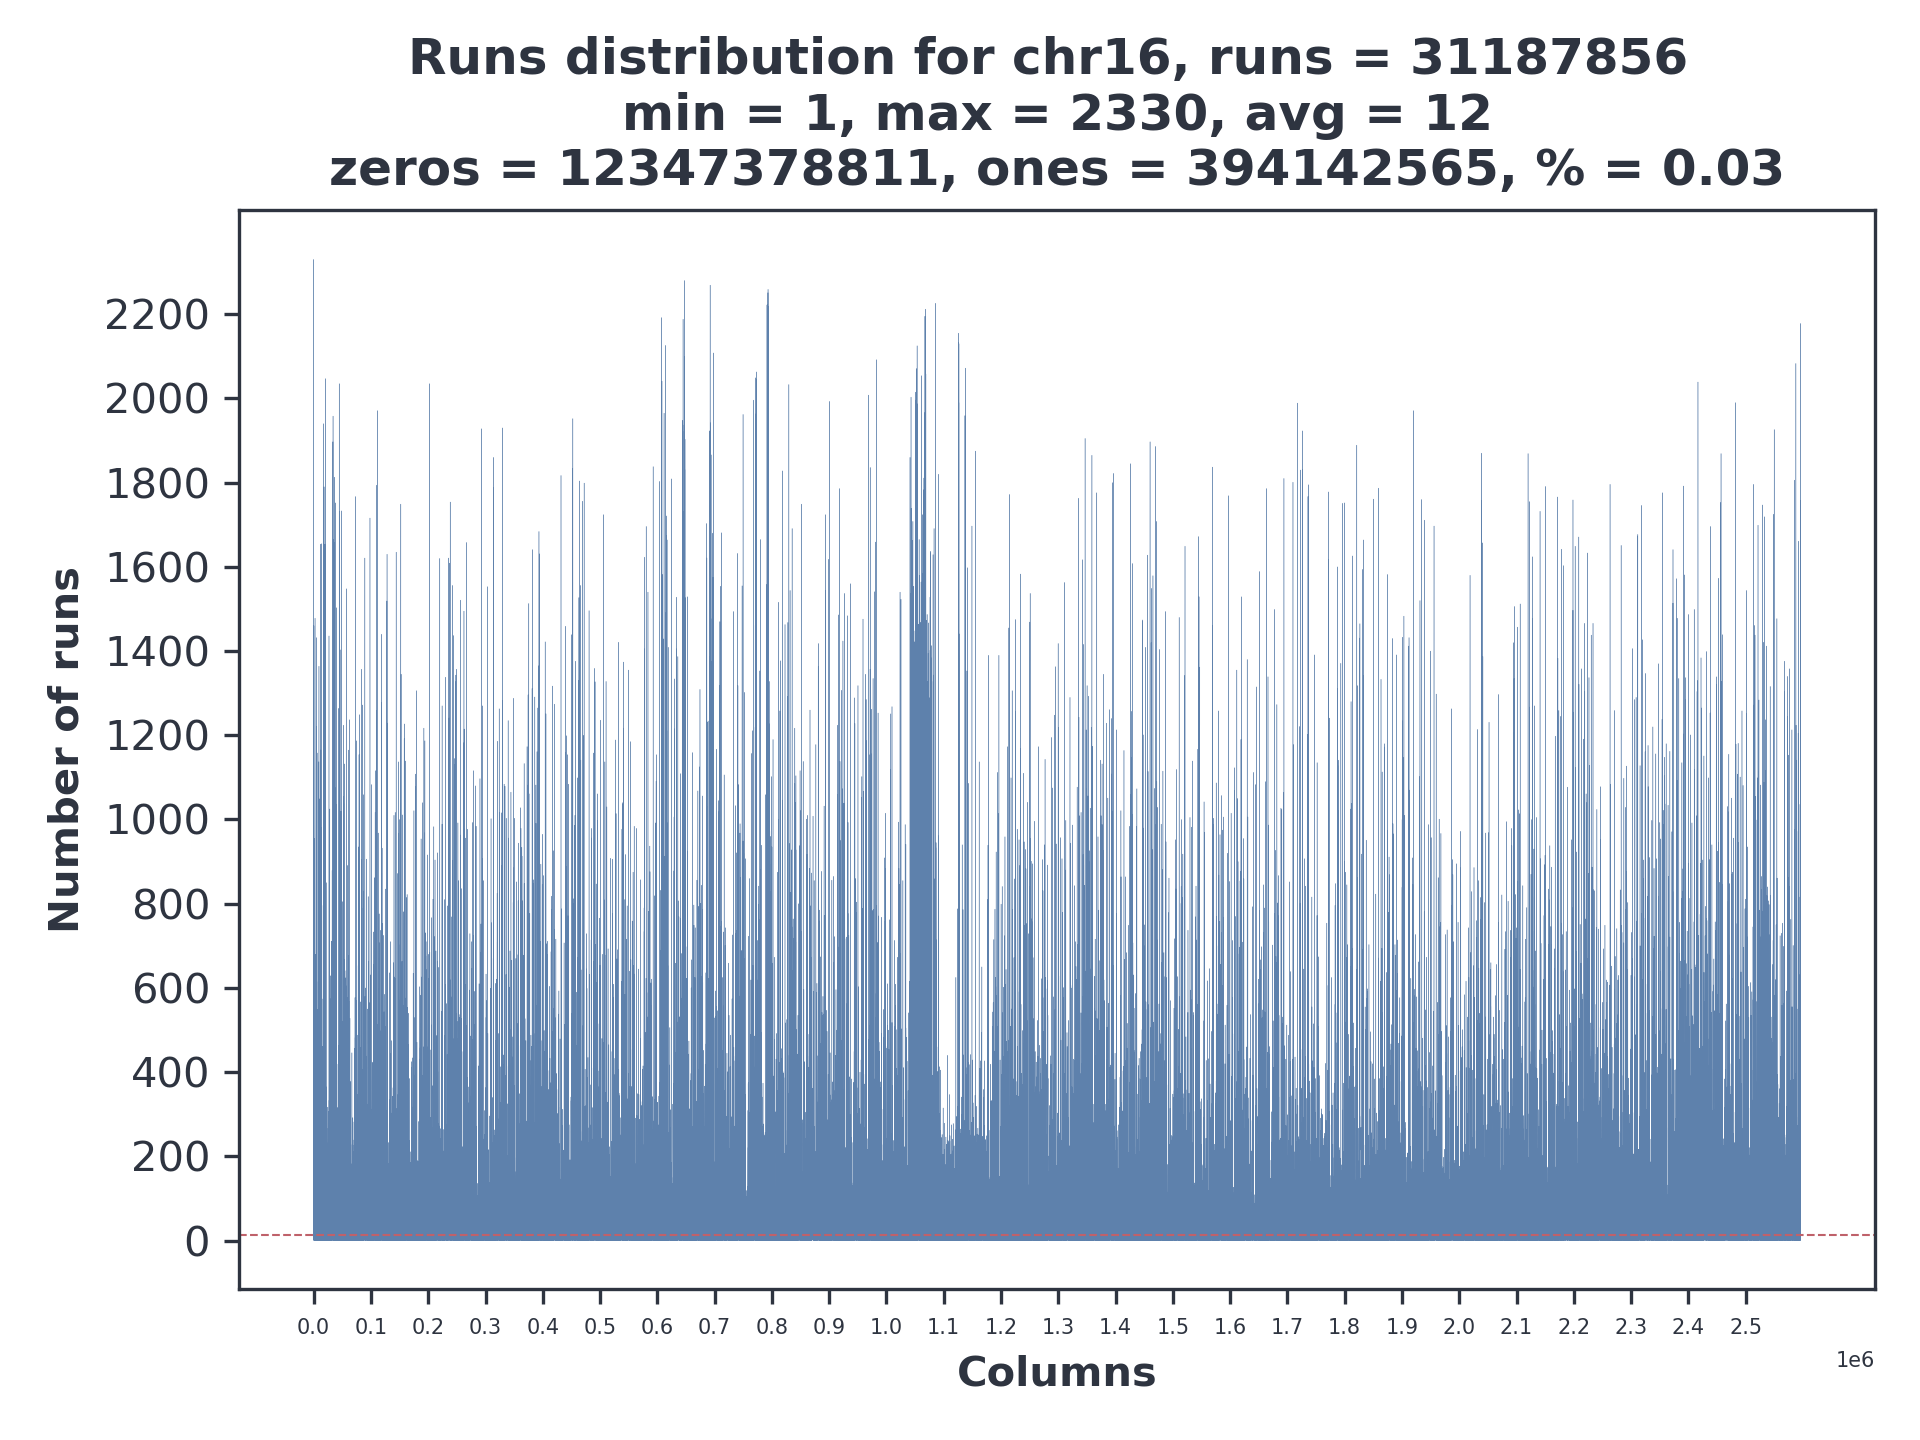
\includegraphics[width=\linewidth]{img/16_runs.png}
  \end{subfigure}
  \begin{subfigure}{.45\textwidth}
    \centering
    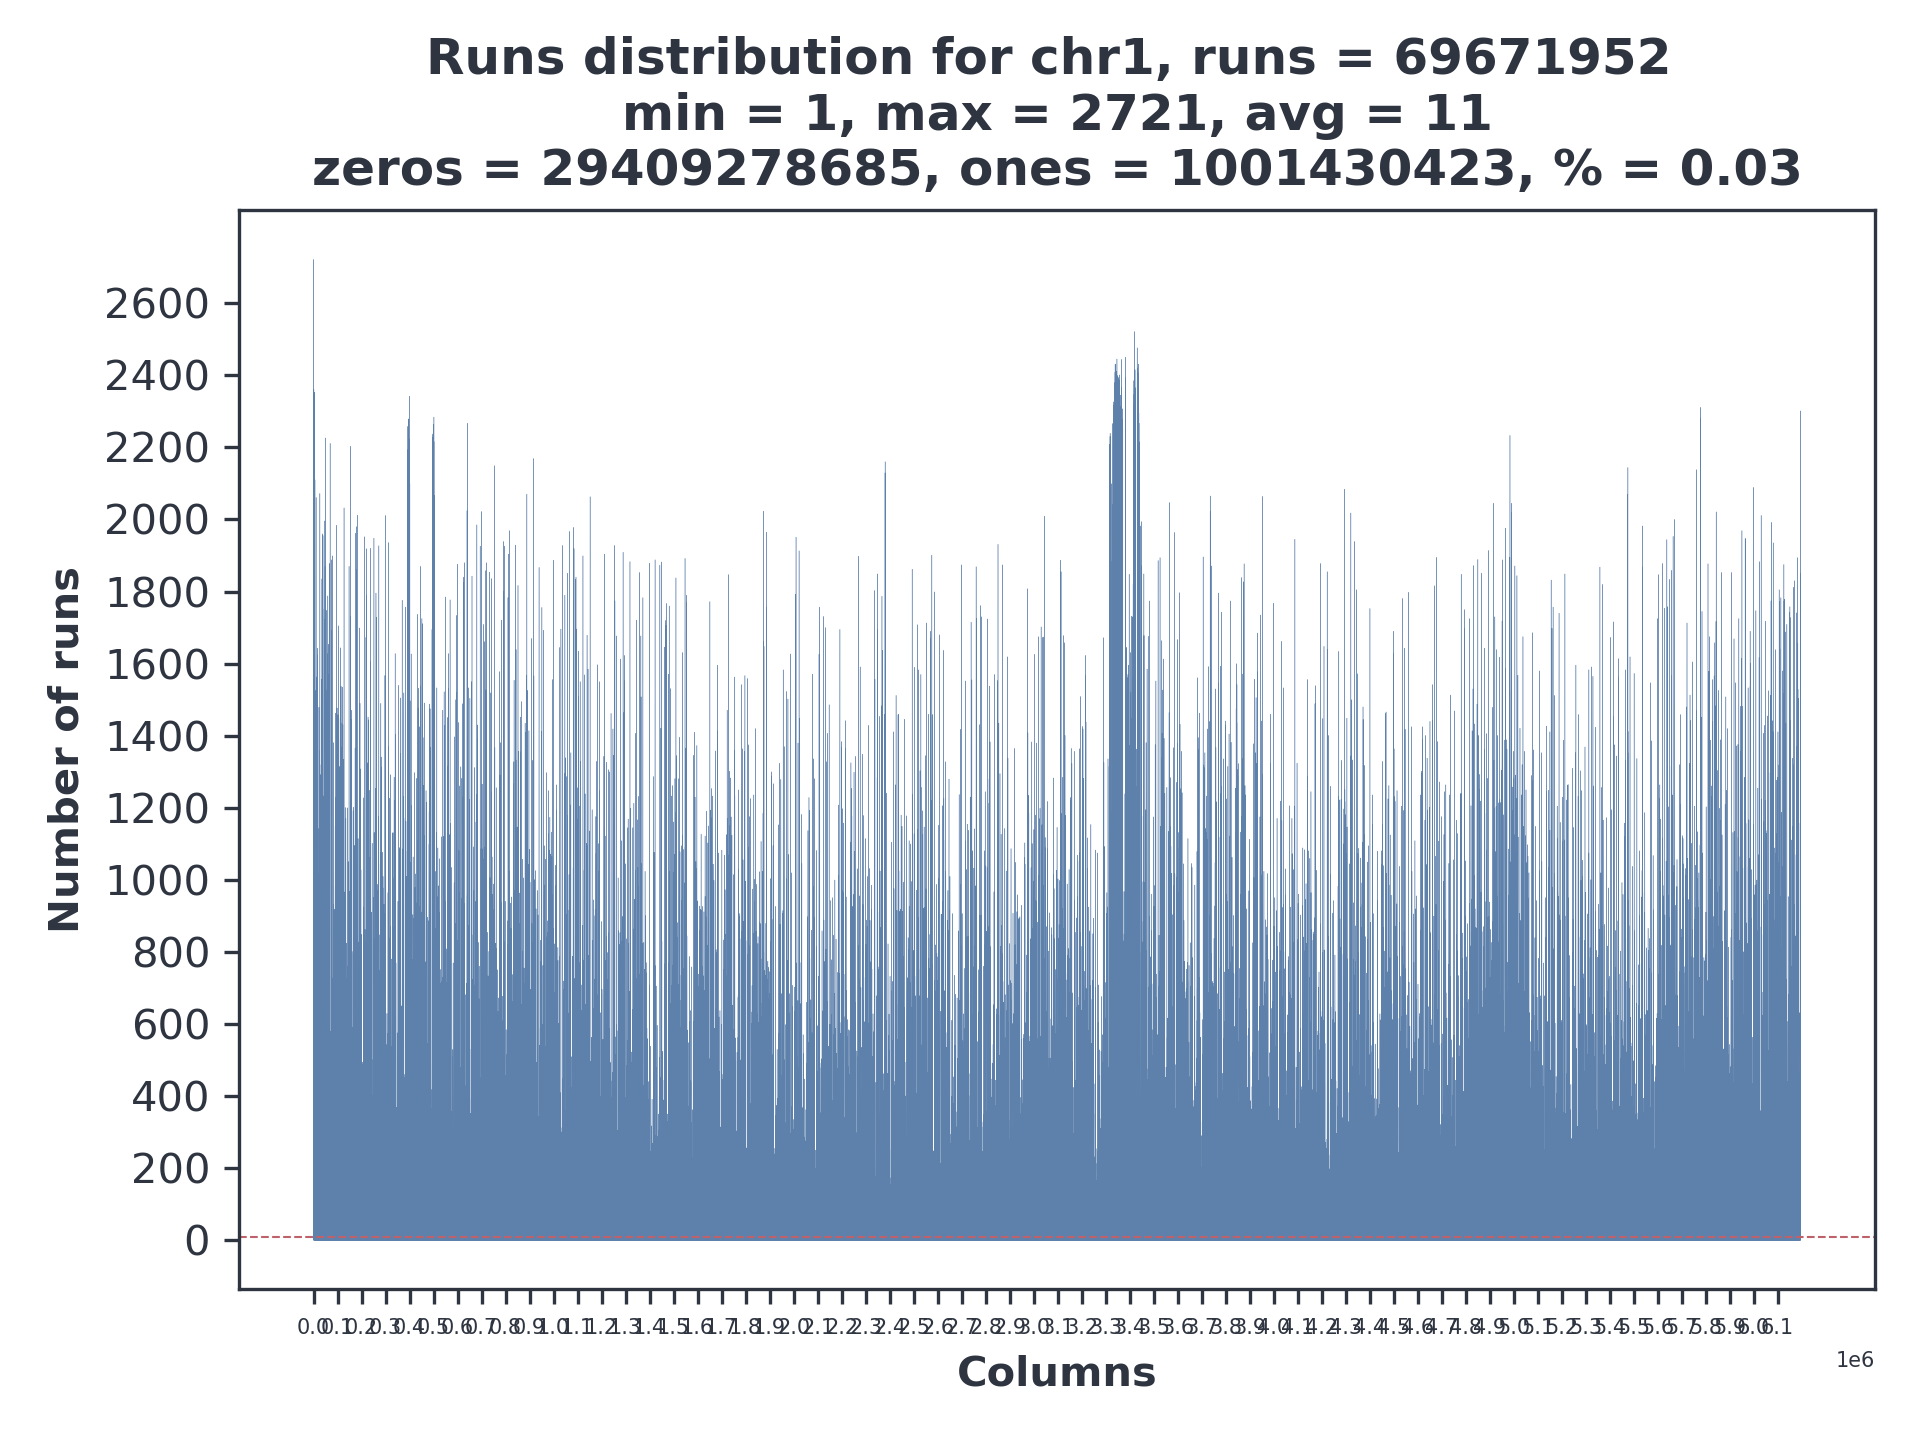
\includegraphics[width=\linewidth]{img/1_runs.png}
  \end{subfigure}
  \caption{Distribuzione delle run per colonna con il numero
    minimo/medio/massimo delle stesse. Nel titolo si hanno anche il numero
    complessivo di run, il numero di simboli $\sigma=0$ e $\sigma=1$, nonché la
    percentuale della quantità di questi ultimi sul totale dei simboli.}
  \label{fig:chrrun}
\end{figure}

Viste le dimensioni di tali pannelli si ritiene necessario studiare, dal punto
di vista del tempo macchina e dei picchi di memoria necessaria, i vari step
della sperimentazione:
\begin{itemize}
  \item la fase di \textit{preprocessing}, necessaria per la \textit{RLPBWT},
  comprendente: 
  \begin{itemize}
    \item la conversione dei file VCF in file MACs
    \item l'estrazione del pannello delle query e la creazione del nuovo
    pannello di reference
    \item la produzione dell\textit{SLP} del pannello di reference, comprendente
    sia la produzione della stringa che l'esecuzione di \textit{BigRepair} che
    di \textit{ShapedSlp}
  \end{itemize}
  \item la costruzione delle varianti della \textit{RLPBWT} e dei file ad hoc
  per la \textit{PBWT}
  \item il calcolo degli SMEMs
\end{itemize}
In generale i risultati ottenuti risultano essere coerenti con quanto visto nei
pannelli simulati.
\paragraph{Preprocessing}
In figura \ref{fig:prechr} si possono analizzare le prestazioni delle tre
fasi. La separazione del pannello con le query risulta essere assolutamente
ininfluente e, di fatto, anche la conversione tra i due formati (conversione che
diventerebbe non necessaria implementando l'input direttamente da file VCF) non
necessita particolari considerazioni. Bisogna, però, analizzare la costruzione
dell'\textit{SLP}. Per quanto quest'operazione sia da svolgersi \textit{una
  tantum}, le richieste in termini di memoria sono nell'ordine delle centinaia
di gigabytes di RAM mentre i tempi di calcolo sono nell'ordine delle
ore. D'altro canto, bisogna considerare che tutti gli algoritmi per la produzione
dell'\textit{SLP} sono studiati per partire da una singola stringa e non da una
matrice e questo potrebbe lasciar spazio a diverse ottimizzazioni. Inoltre
questa fase è necessaria solo per due delle tre soluzioni studiate per la
\textit{RLPBWT} e, come già detto, il fatto che sia necessaria solo una volta
deve essere preso in considerazione nell'ottica di un confronto con, ad esempio,
lo spazio richiesto dall'\textit{algoritmo 5} di Durbin, che richiede $13NM$
bytes ad ogni esecuzione.
\begin{figure}
  \centering
  \begin{subfigure}{.5\textwidth}
    \centering
    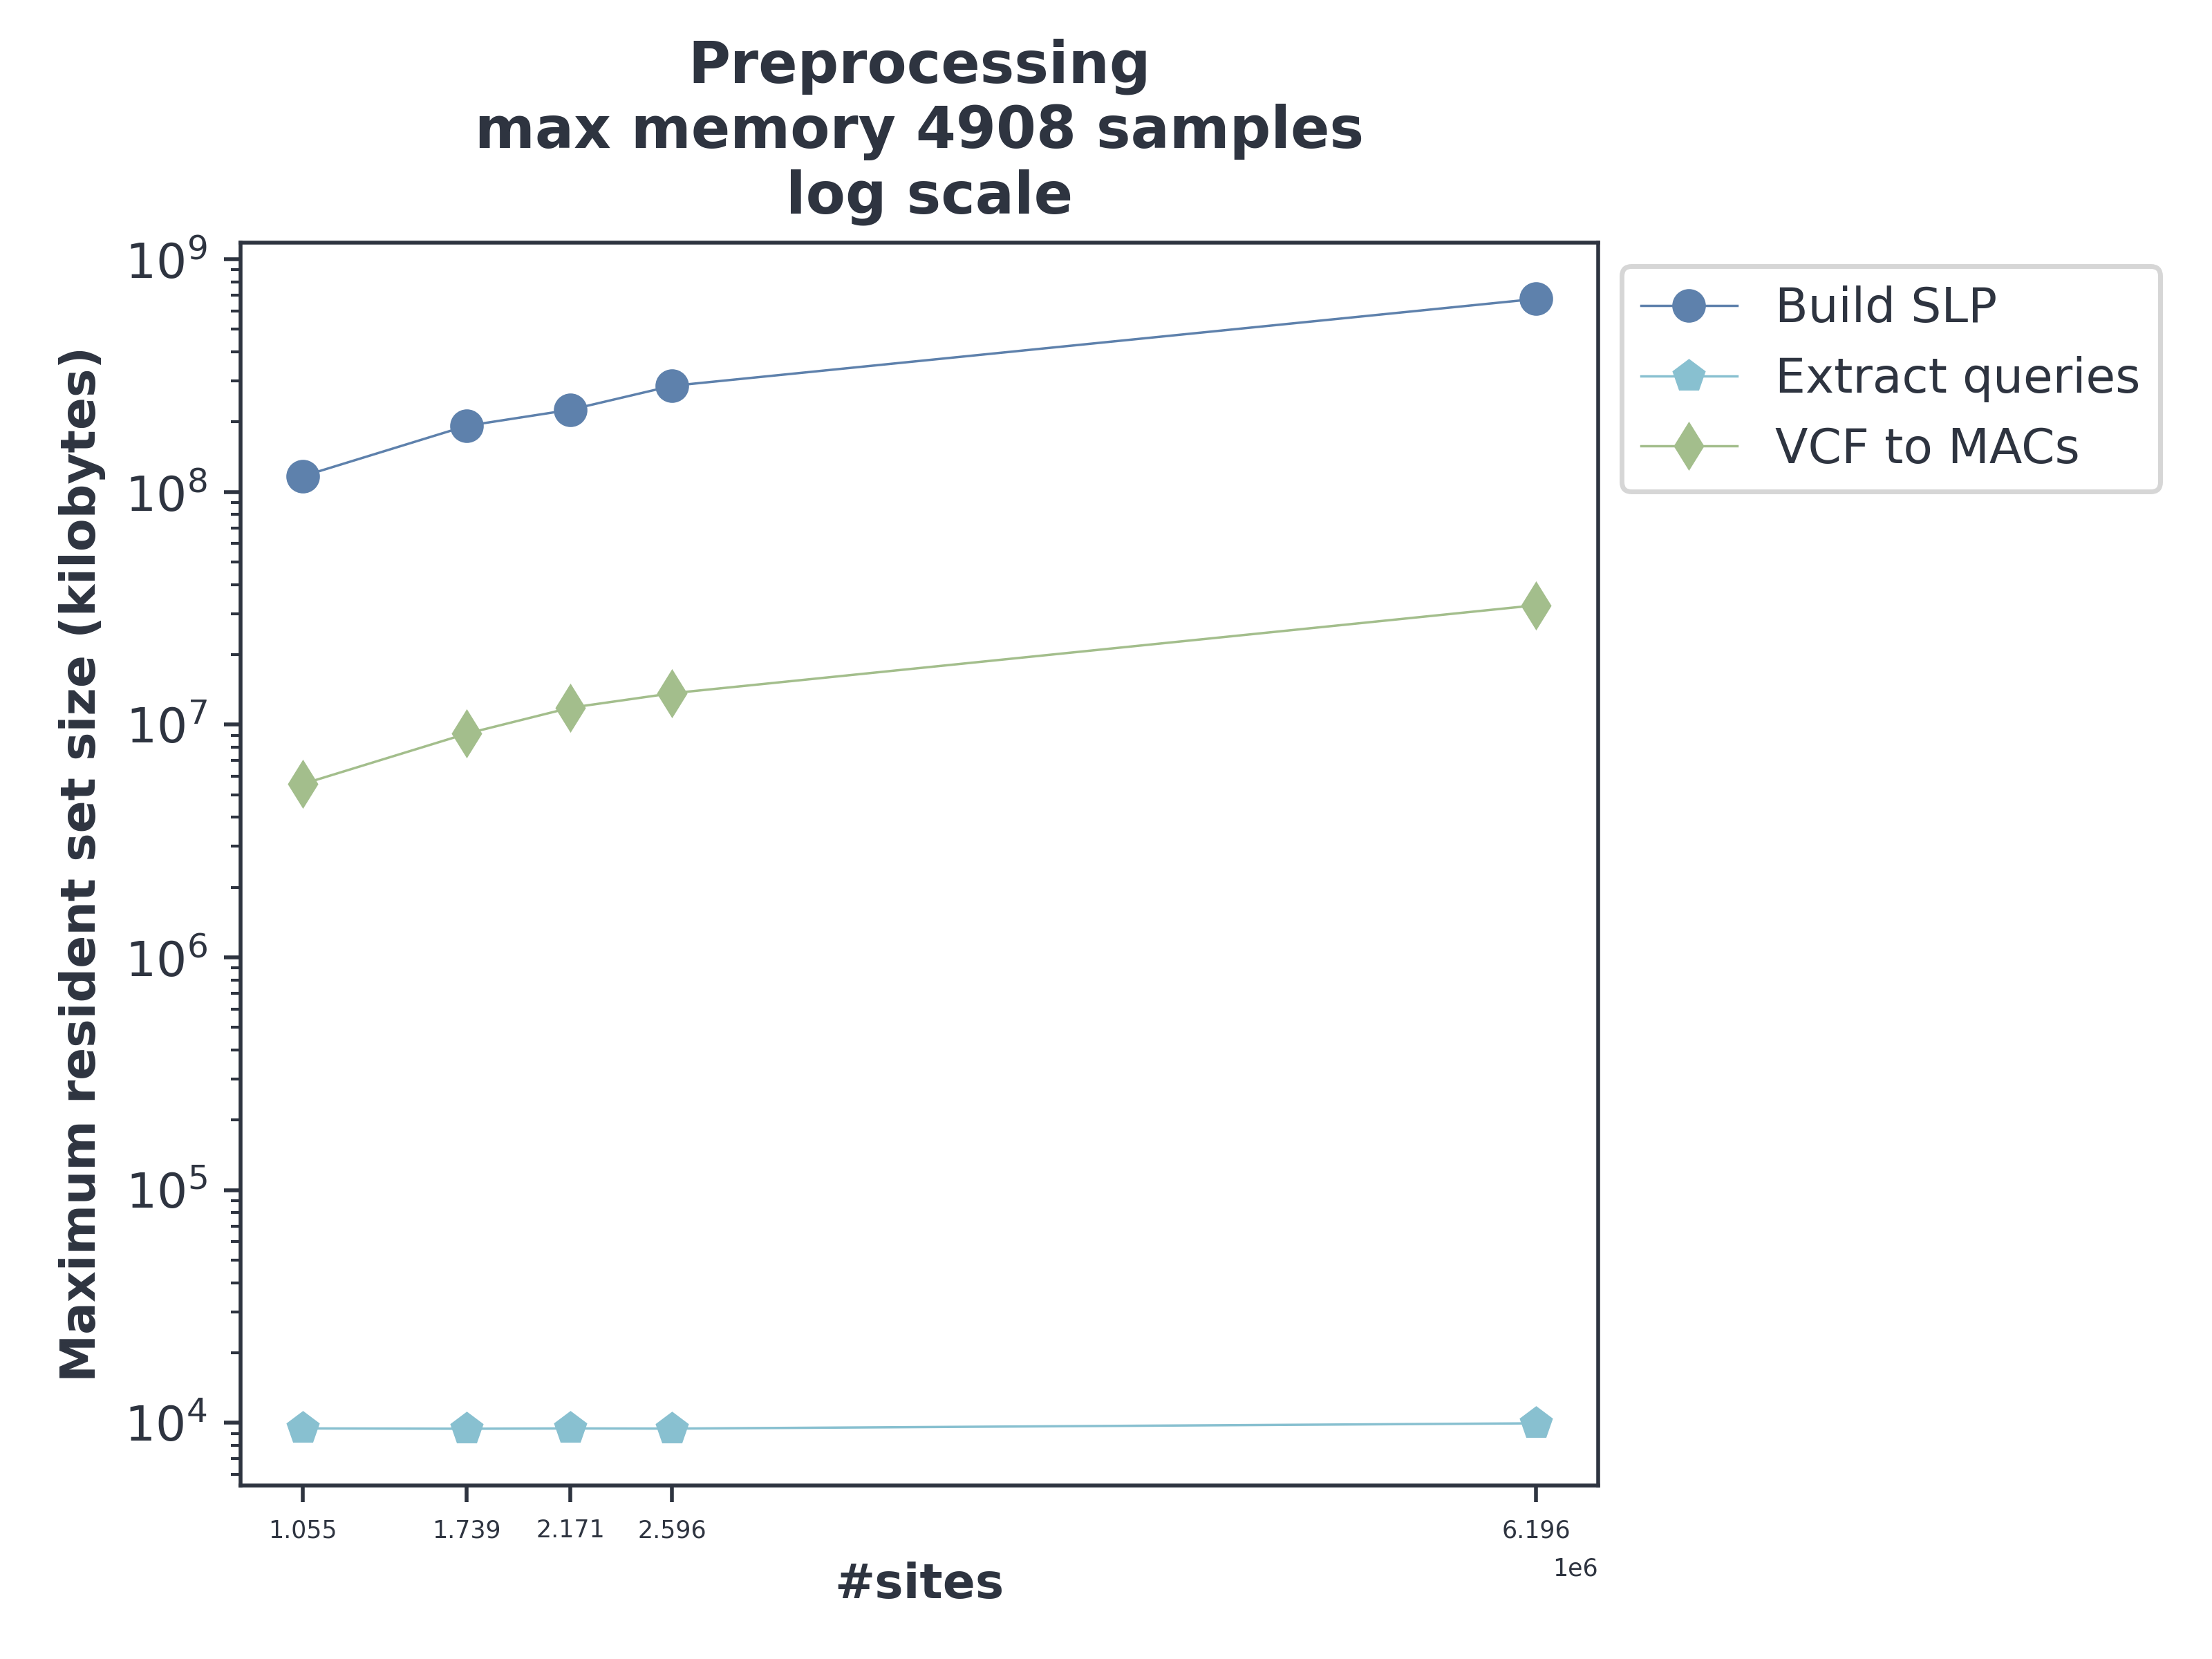
\includegraphics[width=\linewidth]{img/pre_mem_log.png}
  \end{subfigure}%
  \begin{subfigure}{.5\textwidth}
    \centering
    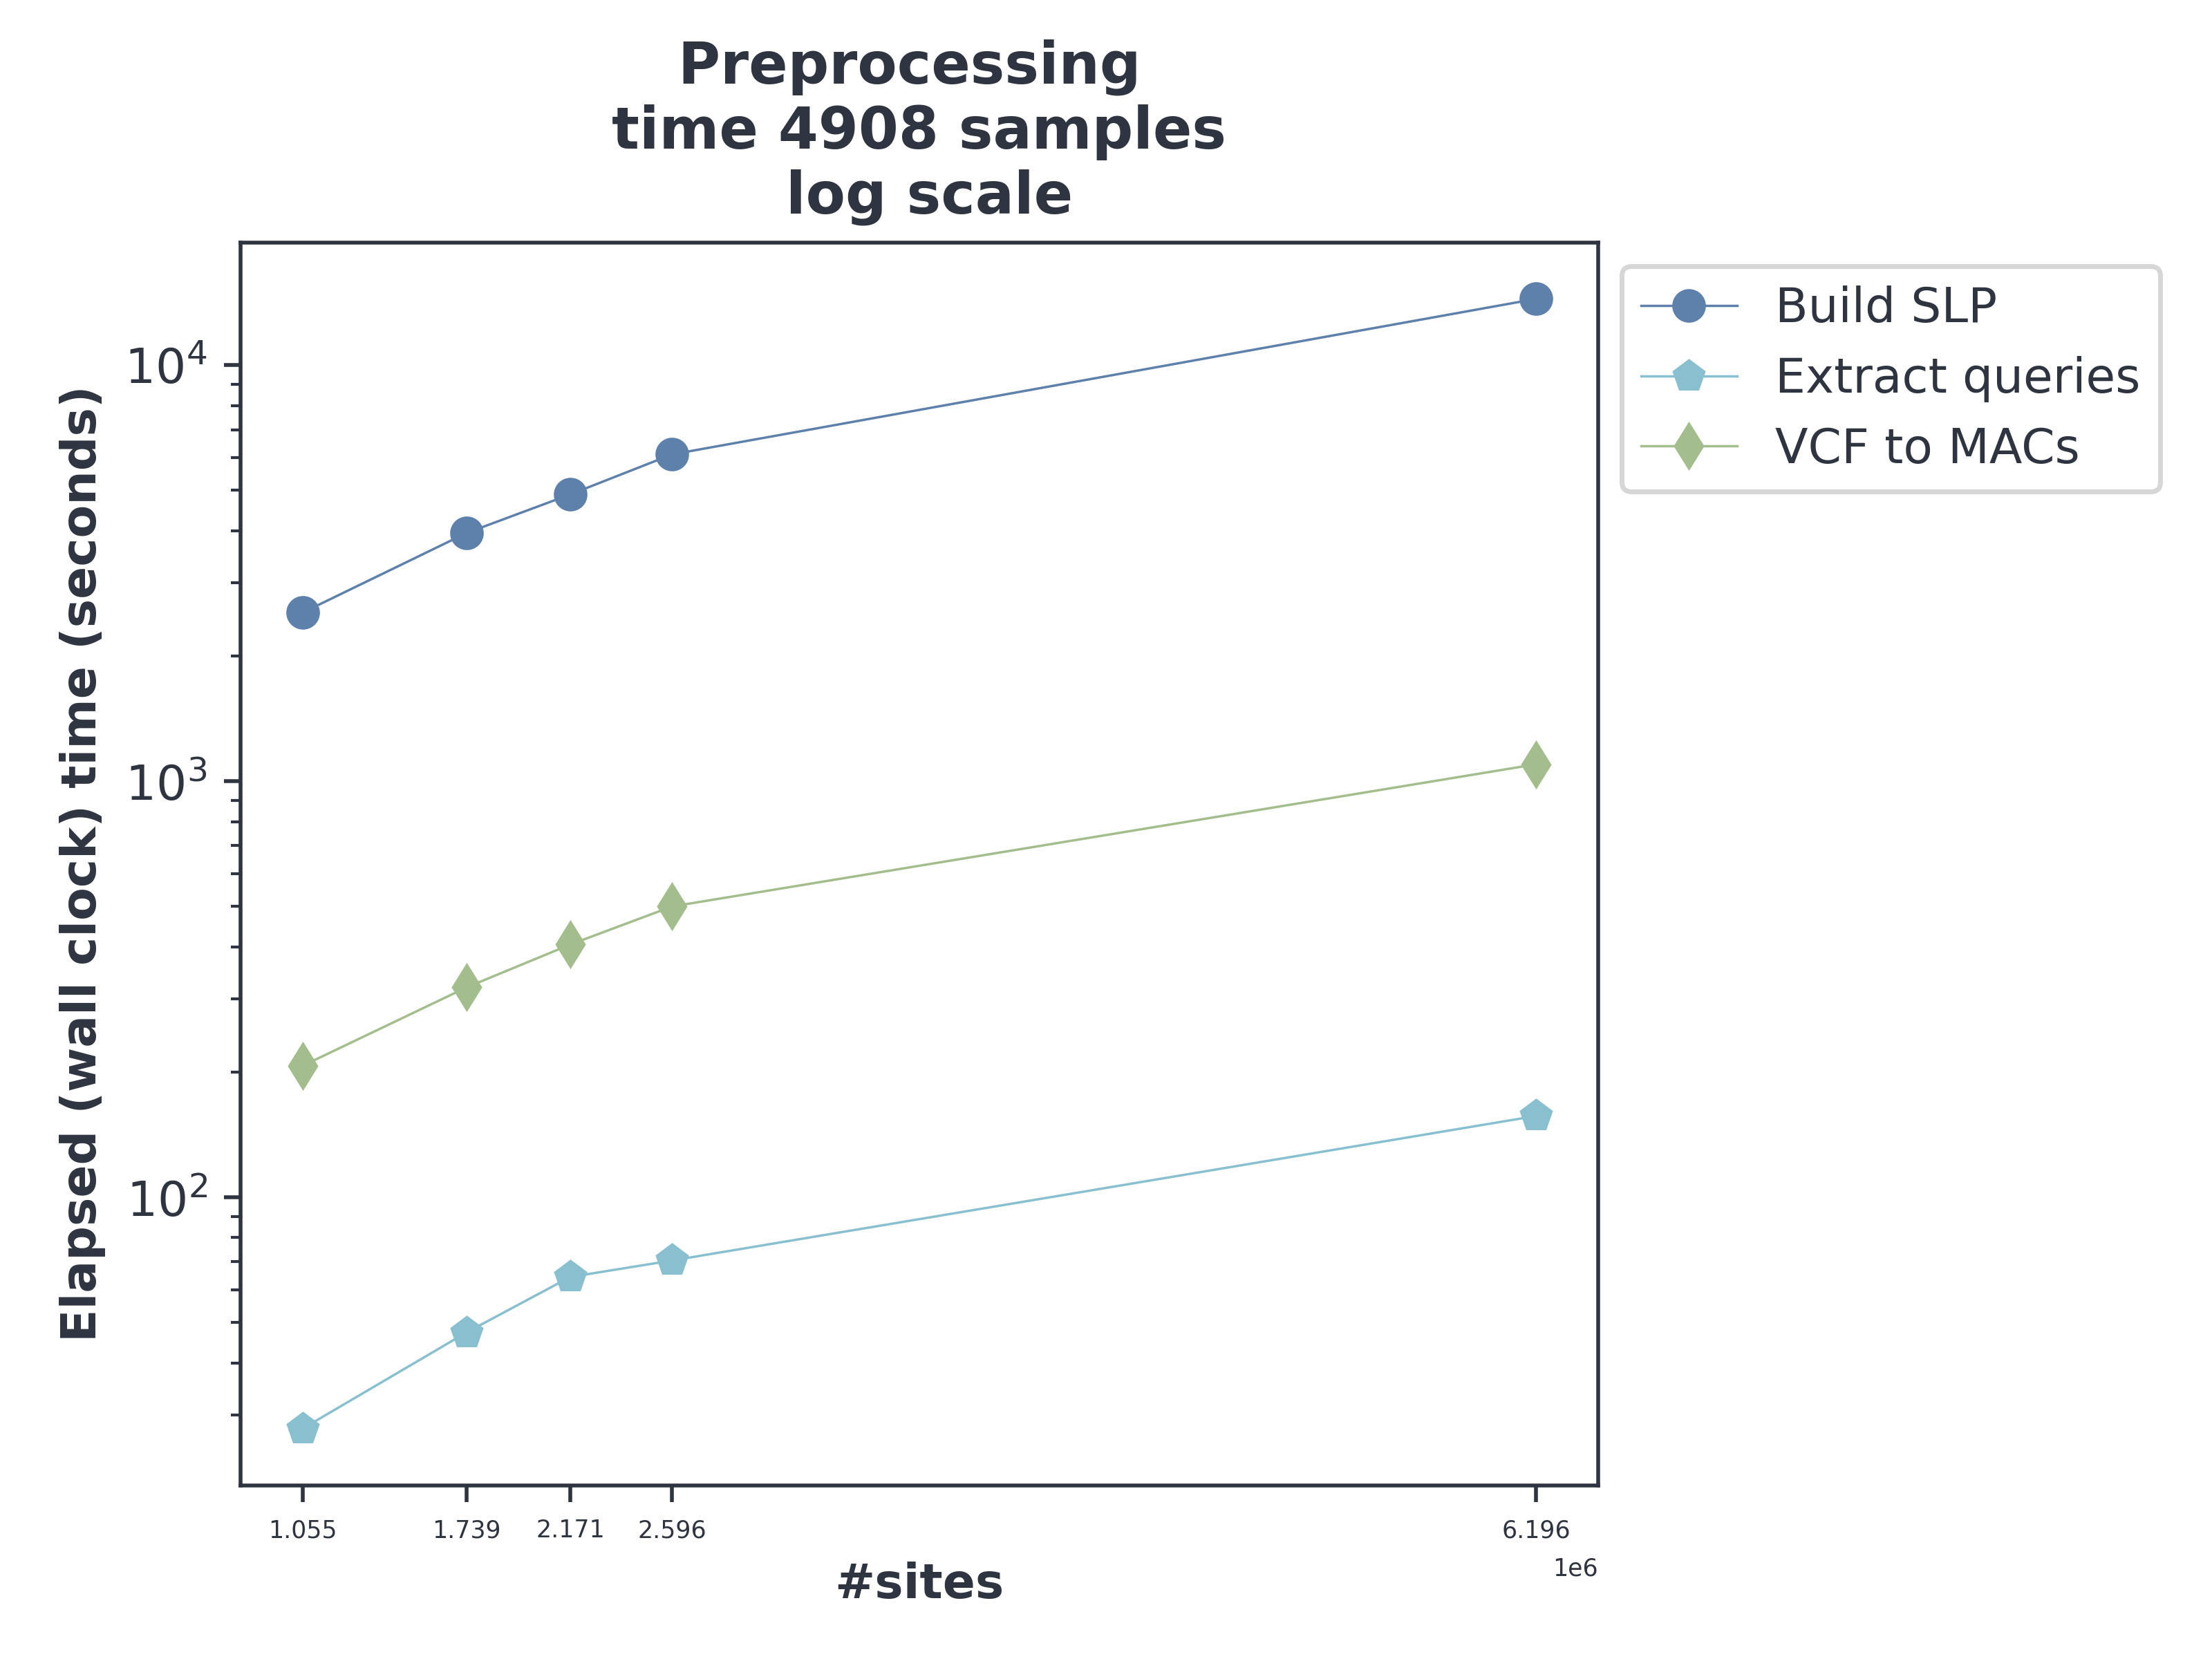
\includegraphics[width=\linewidth]{img/pre_time_log.png}
  \end{subfigure}
  \caption{Tempo richiesto e picco di memoria, in scala logaritmica, per le
    tre fasi di preprocessing 
    dei dati in input per la \textit{RLPBWT}.}
  \label{fig:prechr}
\end{figure}

In figura \ref{fig:slpmacschr} si può osservare il vantaggio in termini di
memoria che si ha con l'uso degli \textit{SLP}, confrontando il peso dei file
MACs con il peso delle grammatiche compresse. Di seguito si possono confrontare
quantitativamente tali risultati, che risultano percentualmente peggiori
rispetto a quanto visto coi pannelli simulati:
\begin{table}[H]
  \centering
  \begin{tabular}{c|c|c|c|c}
    \textbf{\#Samples} & \textbf{\#Siti} & \textbf{SLP (\textit{kb})}
    & \textbf{MACs (\textit{kb})} & \textbf{\%}\\
    \hline
    4908 & 1055454 & 45866.4 & 5079359.44 & 0.9\\
    4908 & 1739315 & 63378.56 & 8370121.94 & 0.76\\
    4908 & 2171378 & 82088.5 & 10449409.15 & 0.79\\
    4908 & 2596072 & 101095.88 & 12493108.91 & 0.81\\
    4908 & 6196151 & 232363.65 & 29821949.72 & 0.78\\
  \end{tabular}
\end{table}
Nonostante tale peggioramento la potenza di compressione degli \textup{SLP}
risulta comunque non trascurabile.
\begin{figure}
  \centering
  \begin{subfigure}{.5\textwidth}
    \centering
    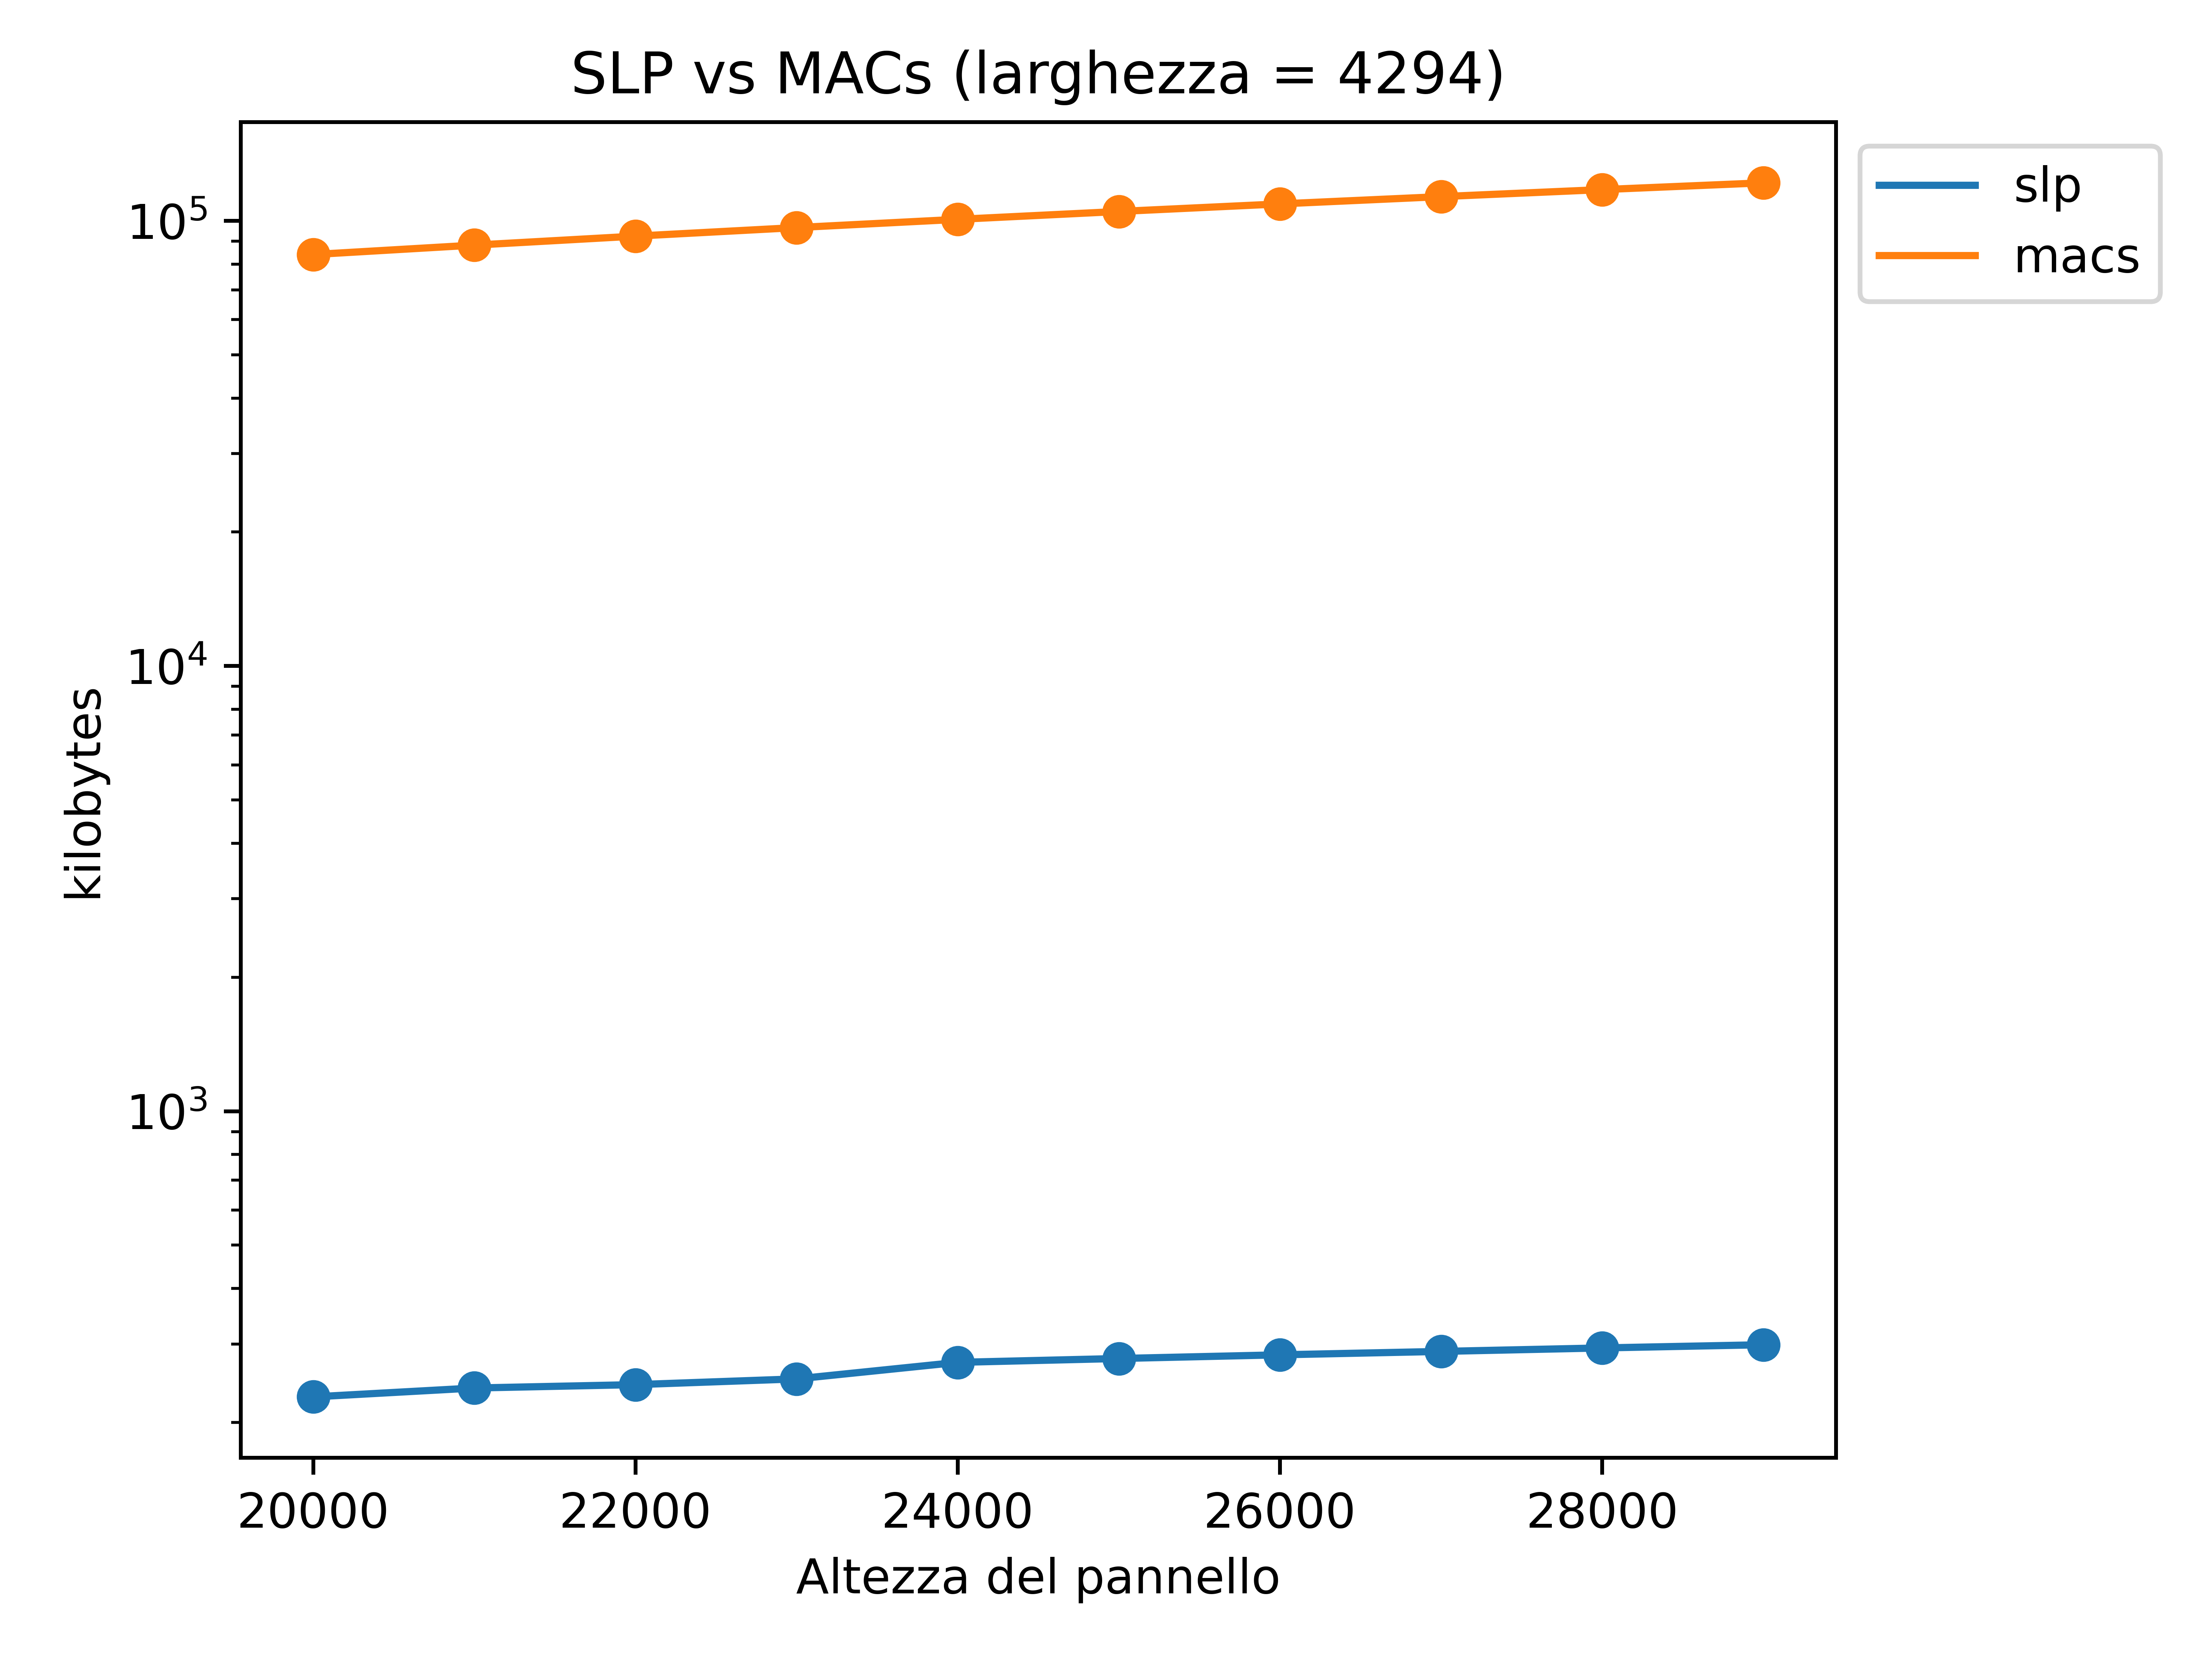
\includegraphics[width=\linewidth]{img/slp_vs_macs.png}
  \end{subfigure}%
  \begin{subfigure}{.5\textwidth}
    \centering
    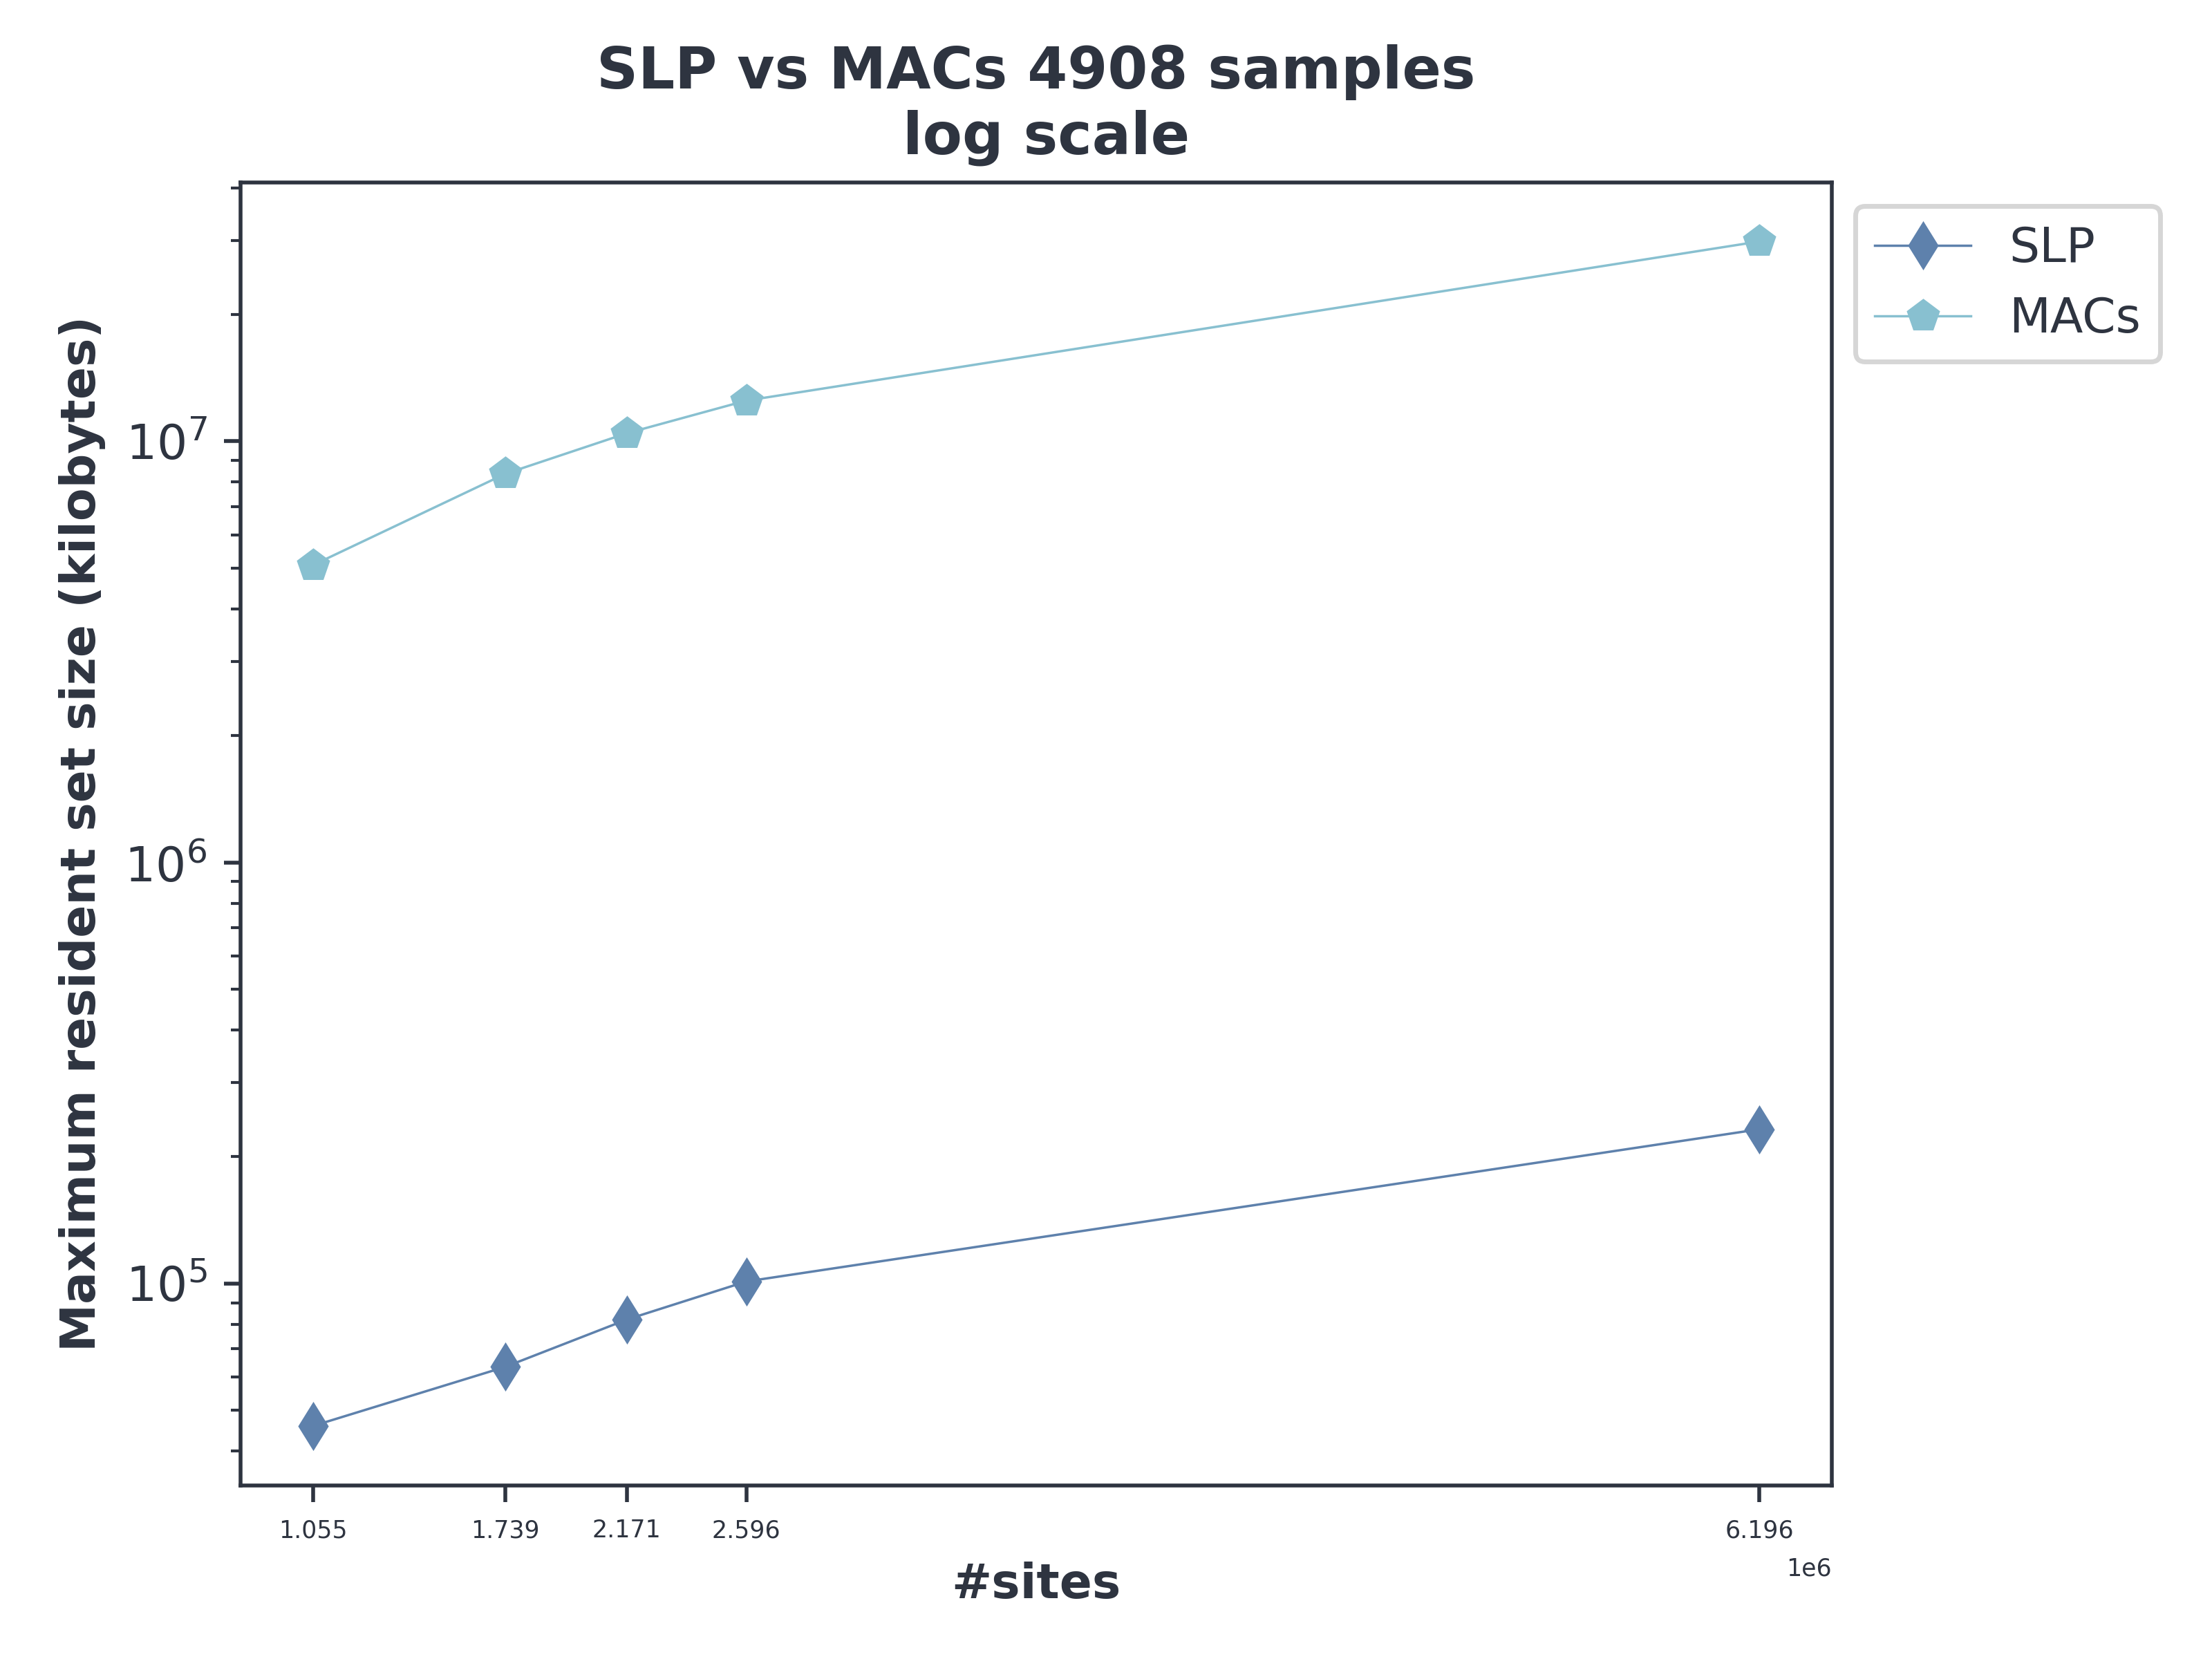
\includegraphics[width=\linewidth]{img/slp_vs_macs_log.png}
  \end{subfigure}
  \caption{Confronto tra la memoria richiesta dai file MACs e dagli SLP per i
    pannelli del 1000 Genome Project. Il grafico di destra è in scala
    logaritmica.} 
  \label{fig:slpmacschr}
\end{figure}
\paragraph{Costruzione della struttura}
Passiamo ora ad analizzare tempi e picchi di memoria per la costruzione delle
strutture dati. Bisogna ricordare che:
\begin{itemize}
  \item nel caso della \textit{RLPBWT} questa fase prevede la costruzione e la
  serializzazione dell'intera struttura dati, comprensiva di tutte le
  sottostrutture necessarie al computo degli SMEM
  \item nel caso della \textit{PBWT} questa fase crea unicamente un file
  compresso ``ad hoc'' con le strutture base delle \textit{PBWT}, a partire
  dalla quale, in fase di calcolo degli SMEM, verranno calcolati anche tutte le
  altre strutture necessarie al calcolo degli stessi
\end{itemize}
Fatte queste doverose premesse passiamo ad analizzare, graficamente in figura
\ref{fig:maketimechr}, i tempi di calcolo della costruzione delle strutture
dati. Si possono fare varie osservazioni:
\begin{itemize}
  \item tutti gli algoritmi di costruzione sono in tempo proporzionale a
  $\mathcal{O}(NM)$ ma, come detto, le varianti della \textit{RLPBWT} includono
  in questa fase anche il calcolo delle strutture utili al calcolo degli SMEM
  \item la \textit{RLPBWT} con \textit{pannello completo} e \textit{threshold}
  richiede più tempo in quanto deve memorizzare effettivamente il pannello
  \item la \textit{RLPBWT na\"{i}ve}, non dovendo costruire i \textit{bitvector
    sparsi} e nemmeno le strutture a supporto per \textit{rank/select}, risulta
  essere la più performante parlando delle soluzioni run-length encoded
\end{itemize}
In figura \ref{fig:makememchr} vengono visualizzati, invece, i picchi di memoria
richiesti. Anche in questo caso si hanno varie osservazioni possibili:
\begin{itemize}
  \item come anticipato la PBWT non calcola e memorizza tutti gli indici
  necessari al calcolo degli SMEM in fase di costruzione, avendo quindi una
  bassissima richiesta di memoria in questa fase
  \item la \textit{RLPBWT na\"{i}ve} e la \textit{RLPBWT con bitvector}, dovendo
  memorizzare l'intero insieme degli \textit{array LCP}, hanno un elevato
  consumo di memoria
  \item nonostante la non memorizzazione delle threshold, la \textit{RLPBWT} con
  \textit{SLP} e \textit{LCE} ha un guadagno minimo rispetto a quella con
  \textit{SLP} e \textit{threshold}. Questo è giustificato dalla sparsità dei
  dati (nonché dal conseguente basso numero di run) e dall'uso dei
  \textit{bitvector sparsi}, che scalano in memoria proprio sul numero di
  simboli $\sigma=1$, quindi sul numero di run
\end{itemize}
\begin{figure}
  \centering
  \begin{subfigure}{.5\textwidth}
    \centering
    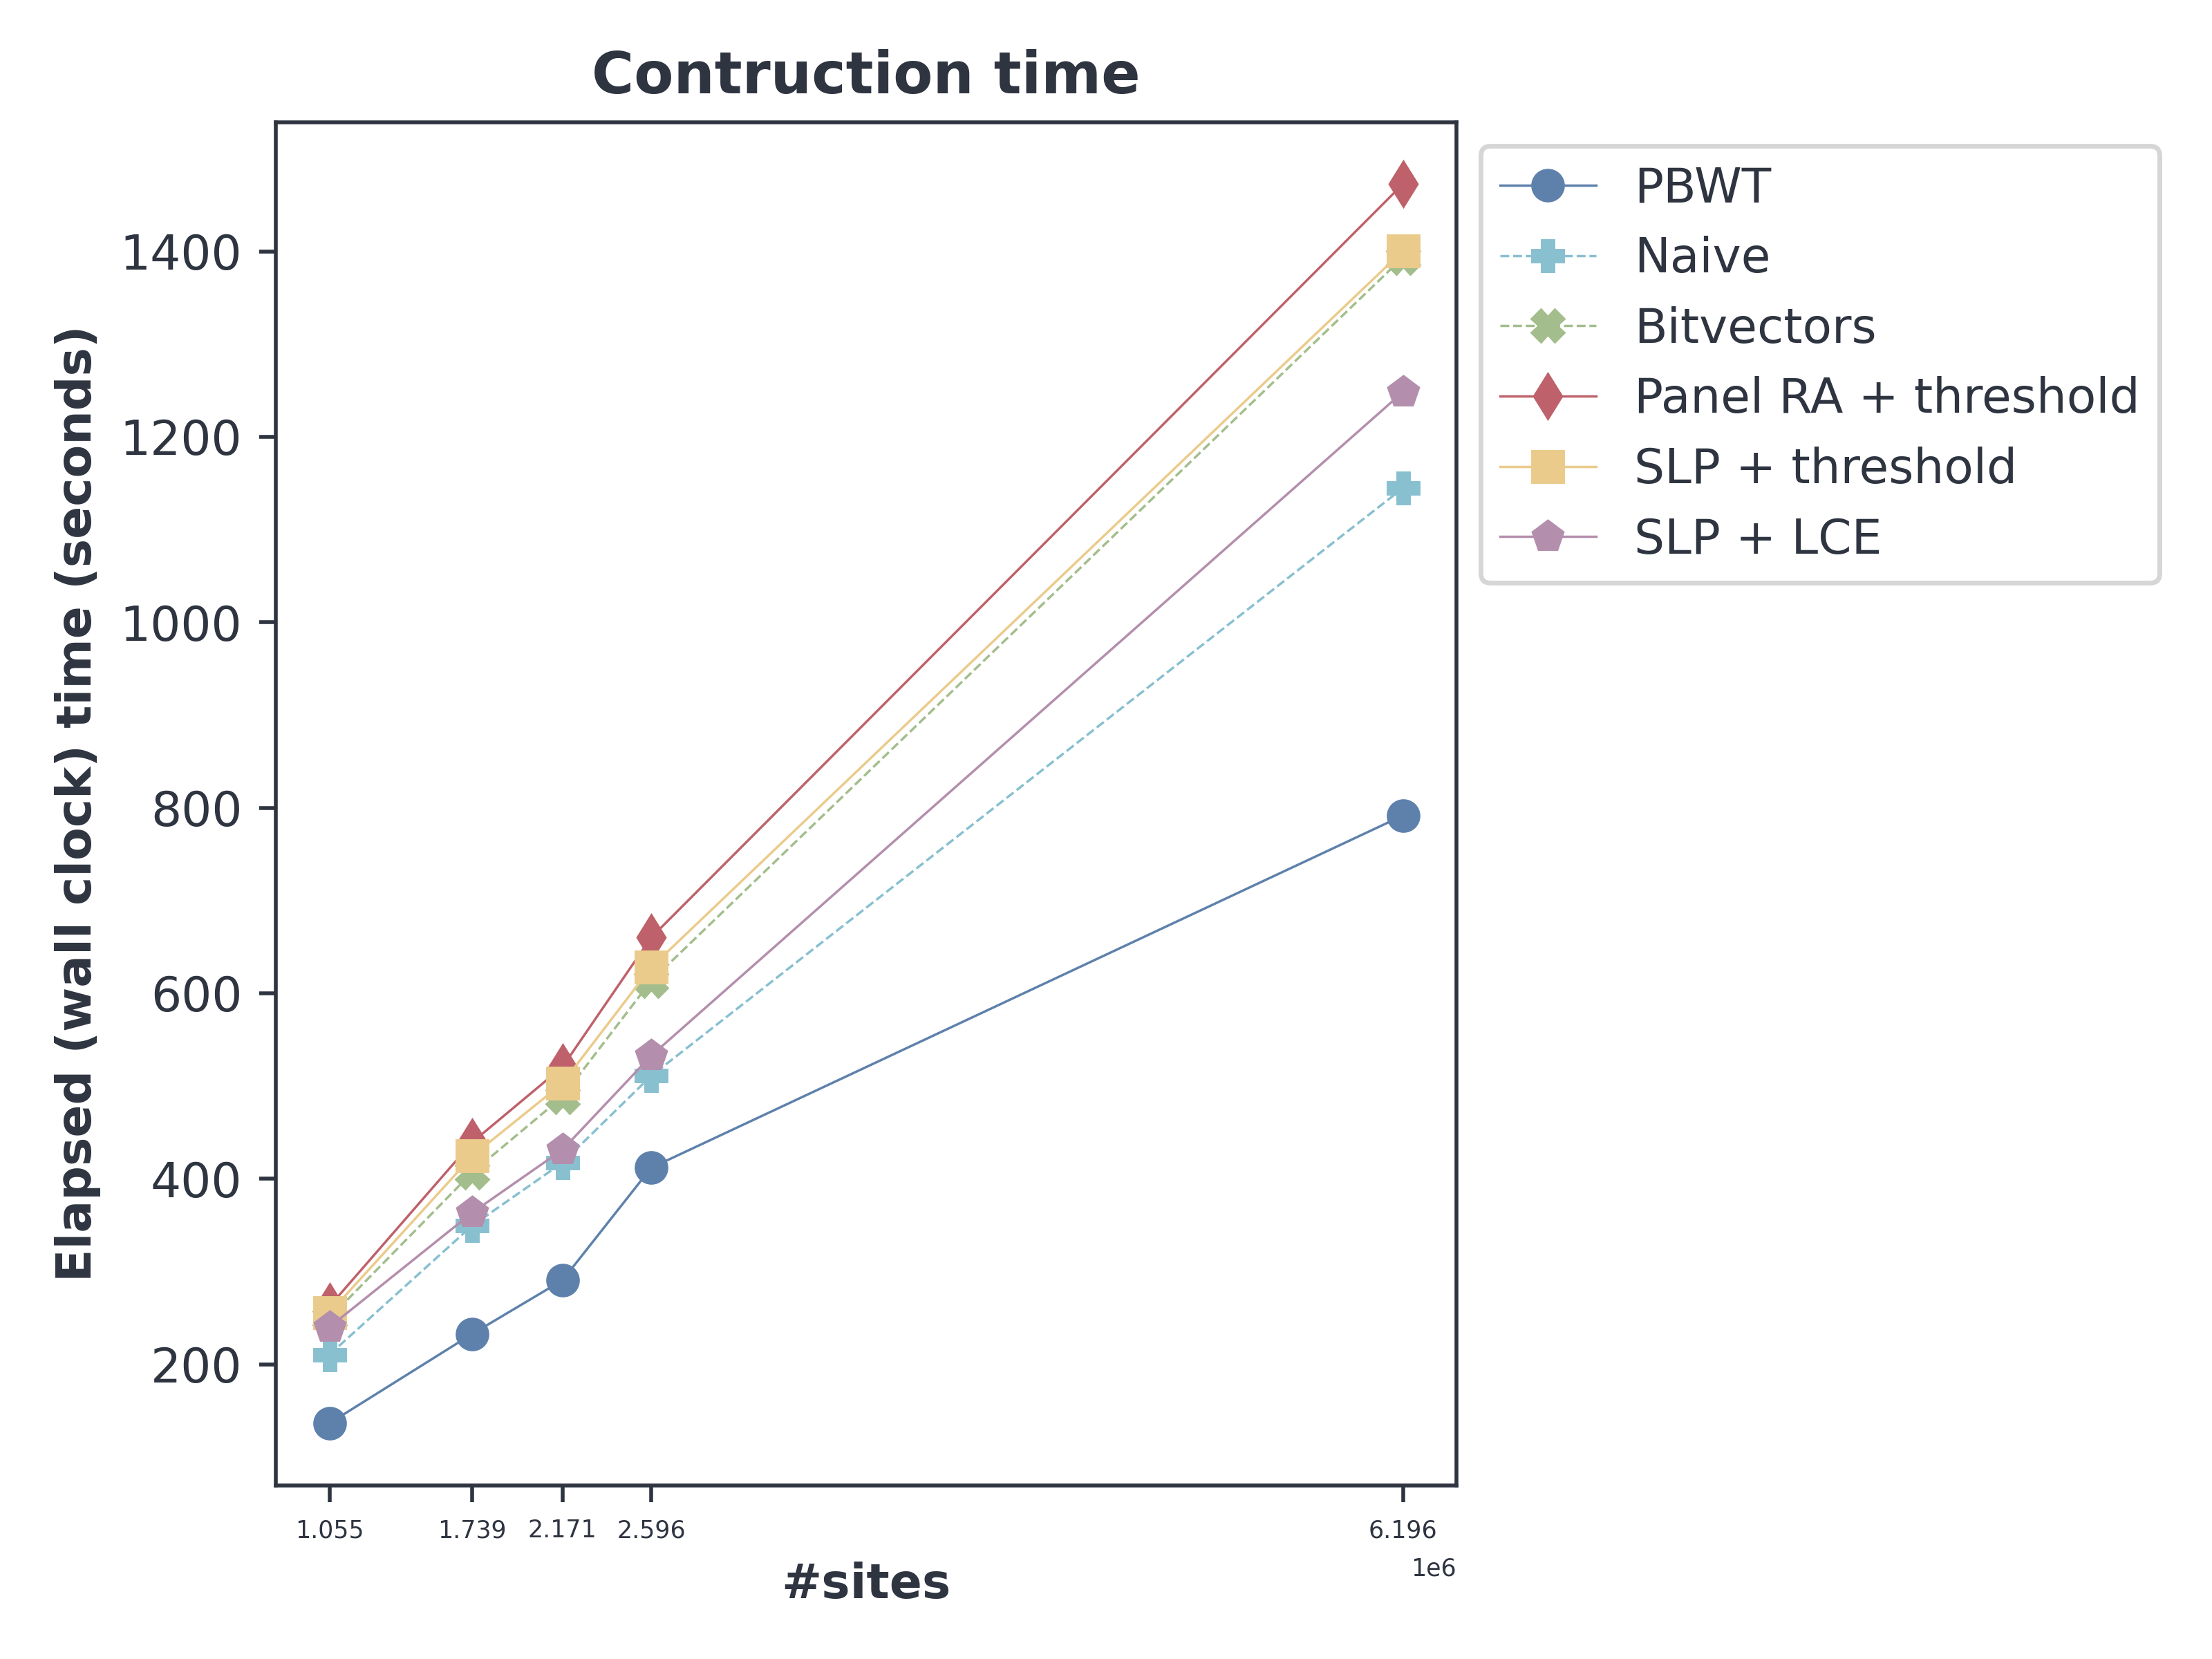
\includegraphics[width=\linewidth]{img/make_time.png}
  \end{subfigure}%
  \begin{subfigure}{.5\textwidth}
    \centering
    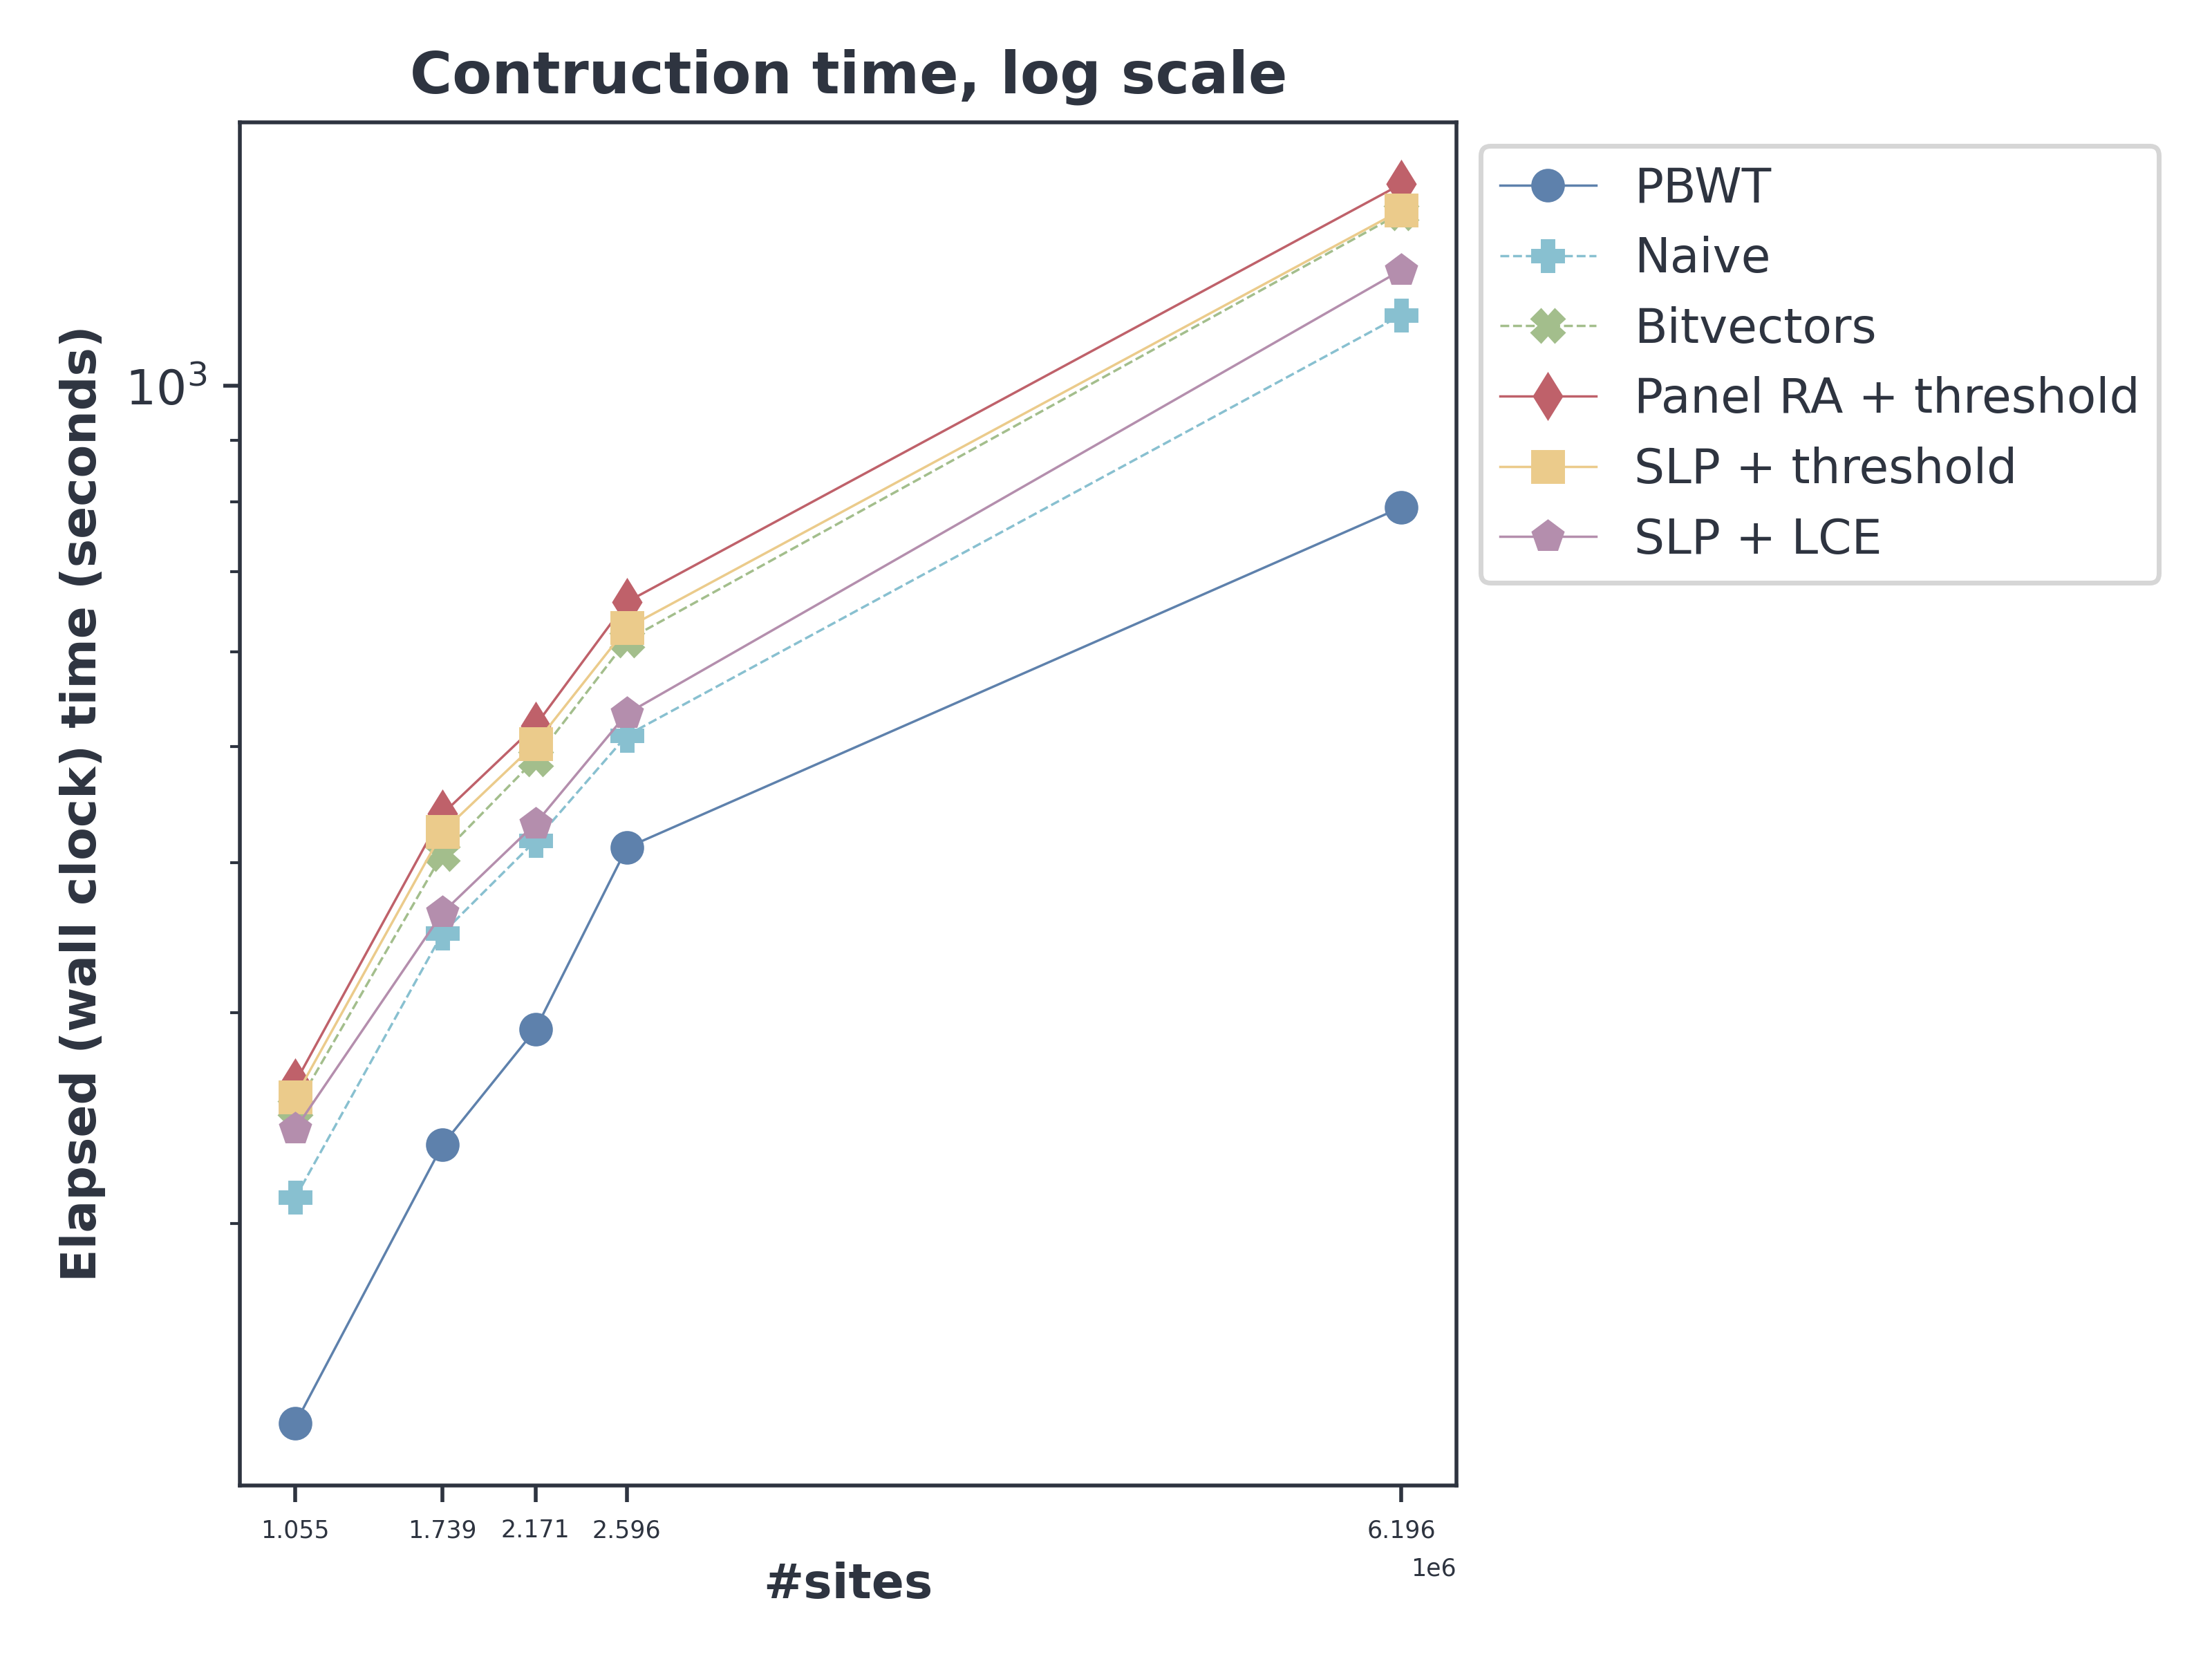
\includegraphics[width=\linewidth]{img/make_time_log.png}
  \end{subfigure}
  \caption{Wall clock time per la costruzione delle varianti della RLPWBT e per
    la PBWT. Il grafico di destra presenta il tempo in scala logaritmica.}
  \label{fig:maketimechr}
\end{figure}
\begin{figure}
  \centering
  \begin{subfigure}{.5\textwidth}
    \centering
    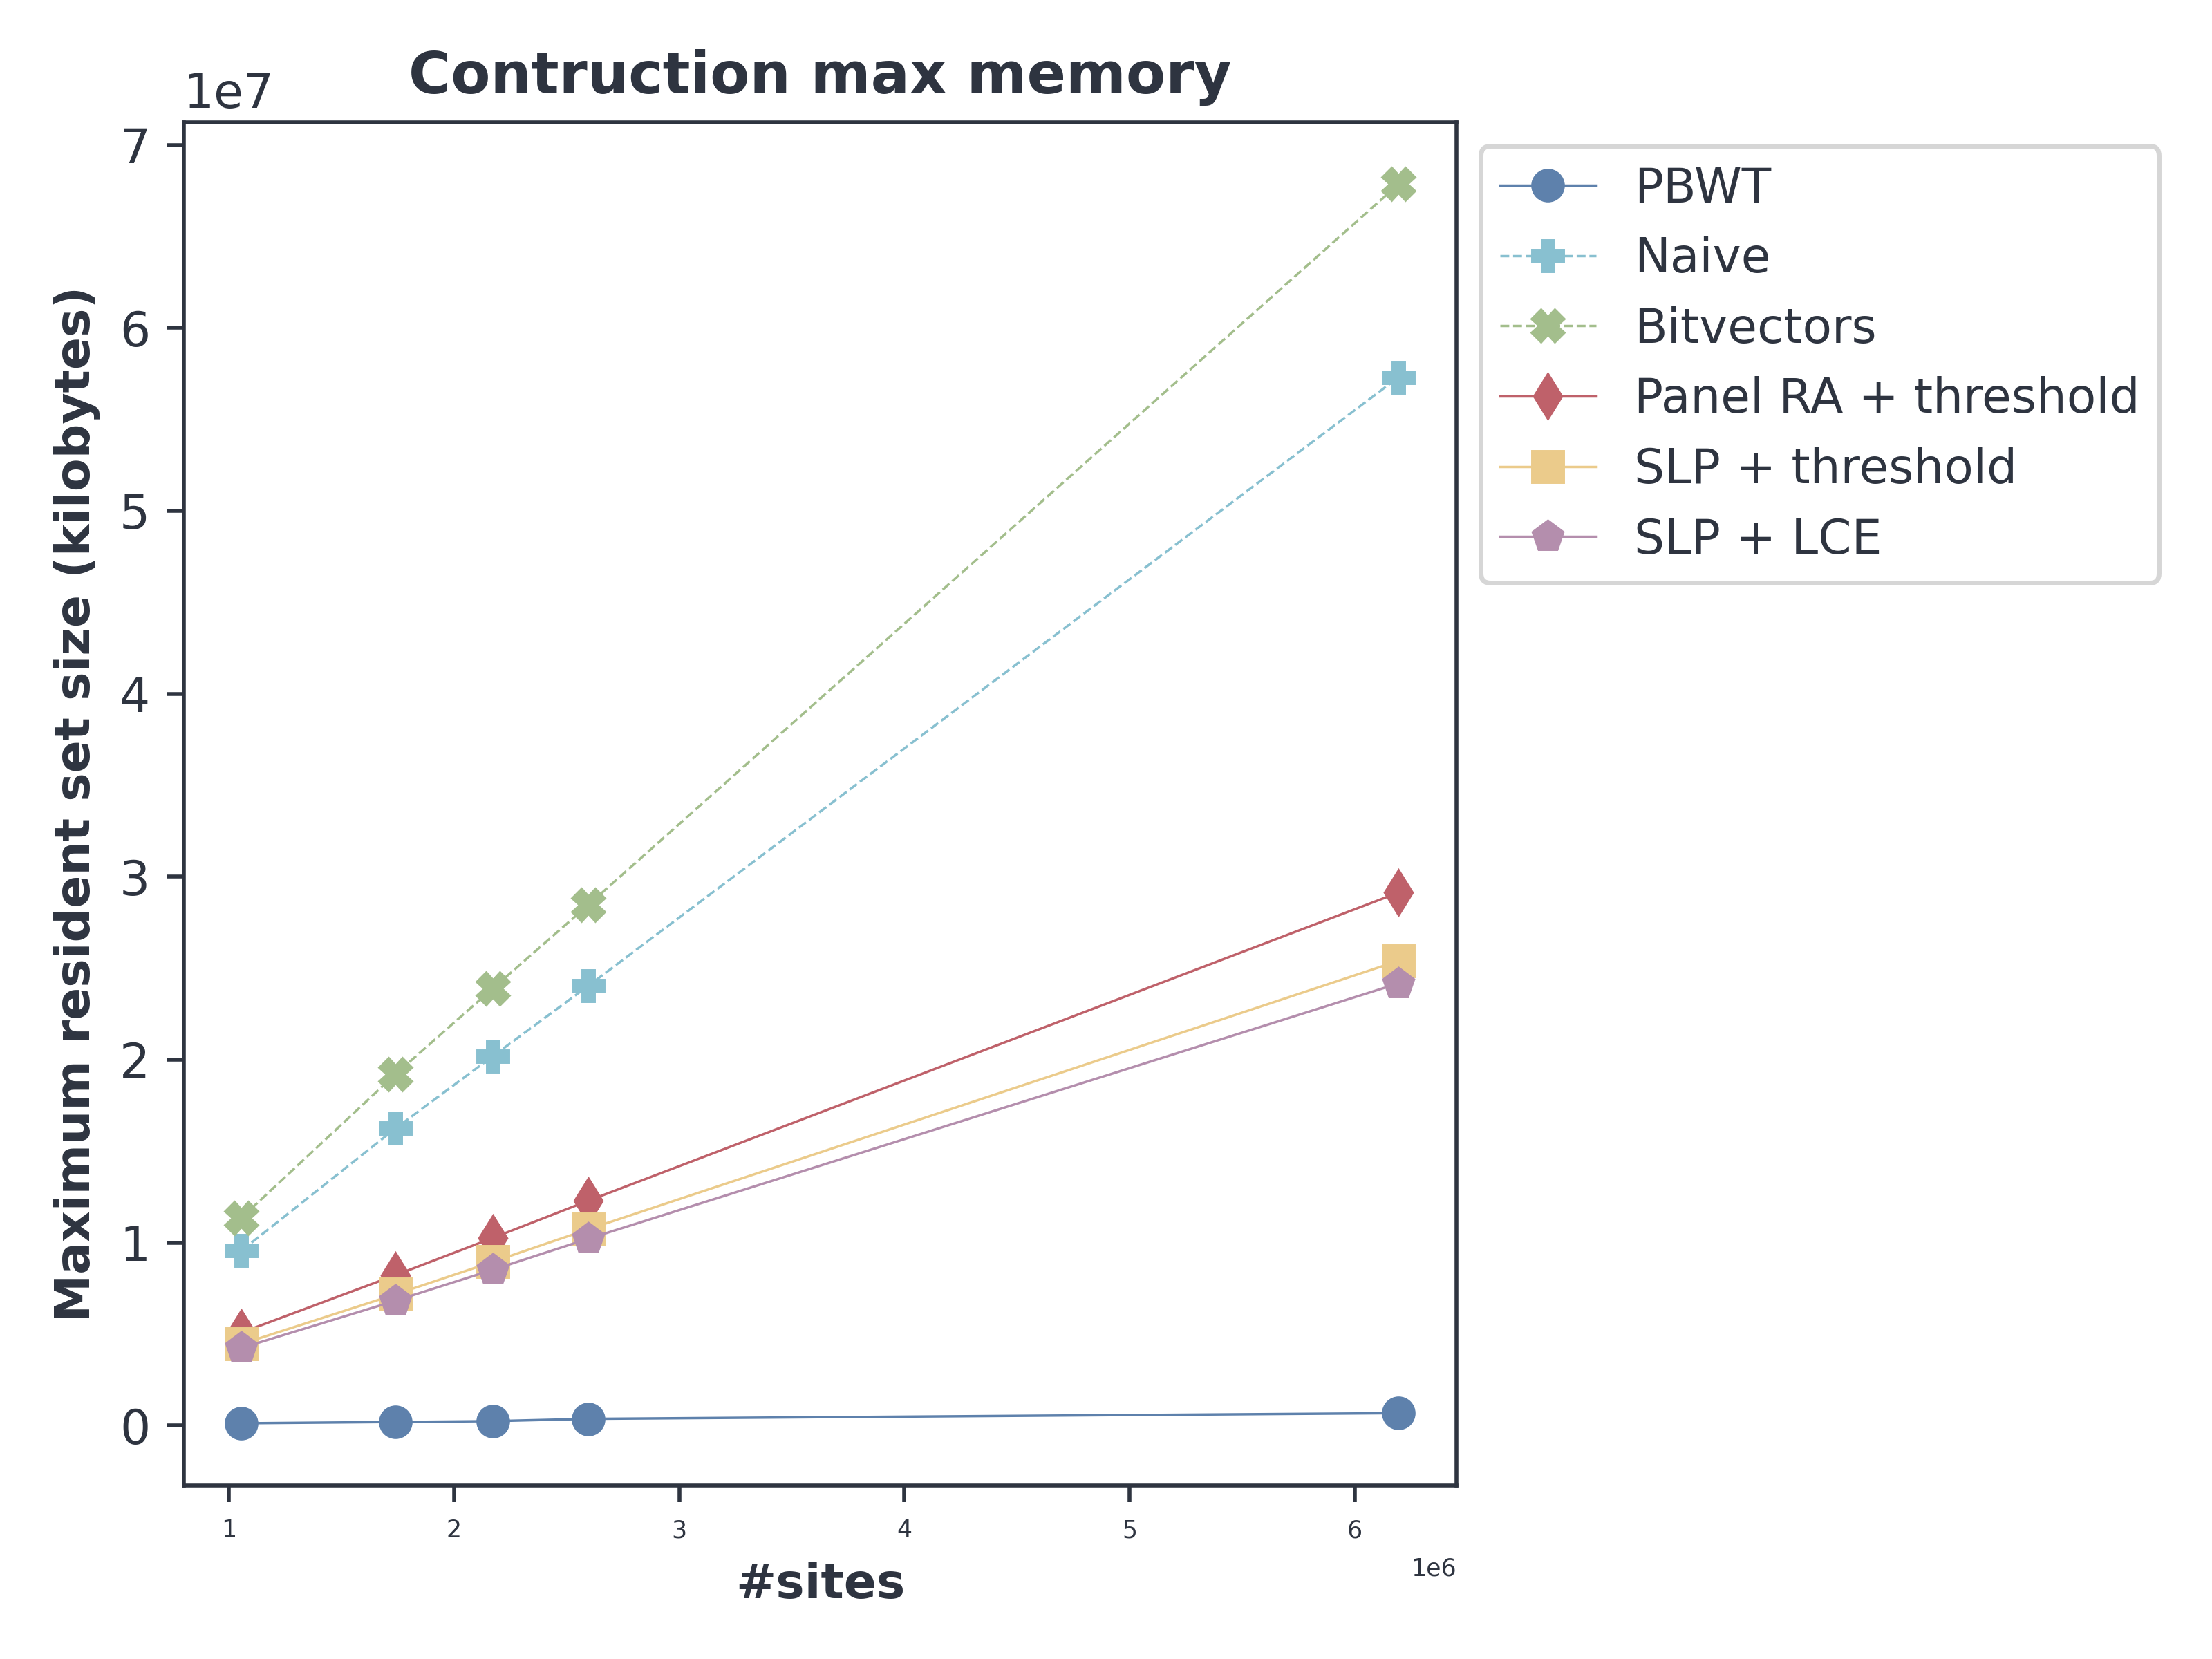
\includegraphics[width=\linewidth]{img/make_mem.png}
  \end{subfigure}%
  \begin{subfigure}{.5\textwidth}
    \centering
    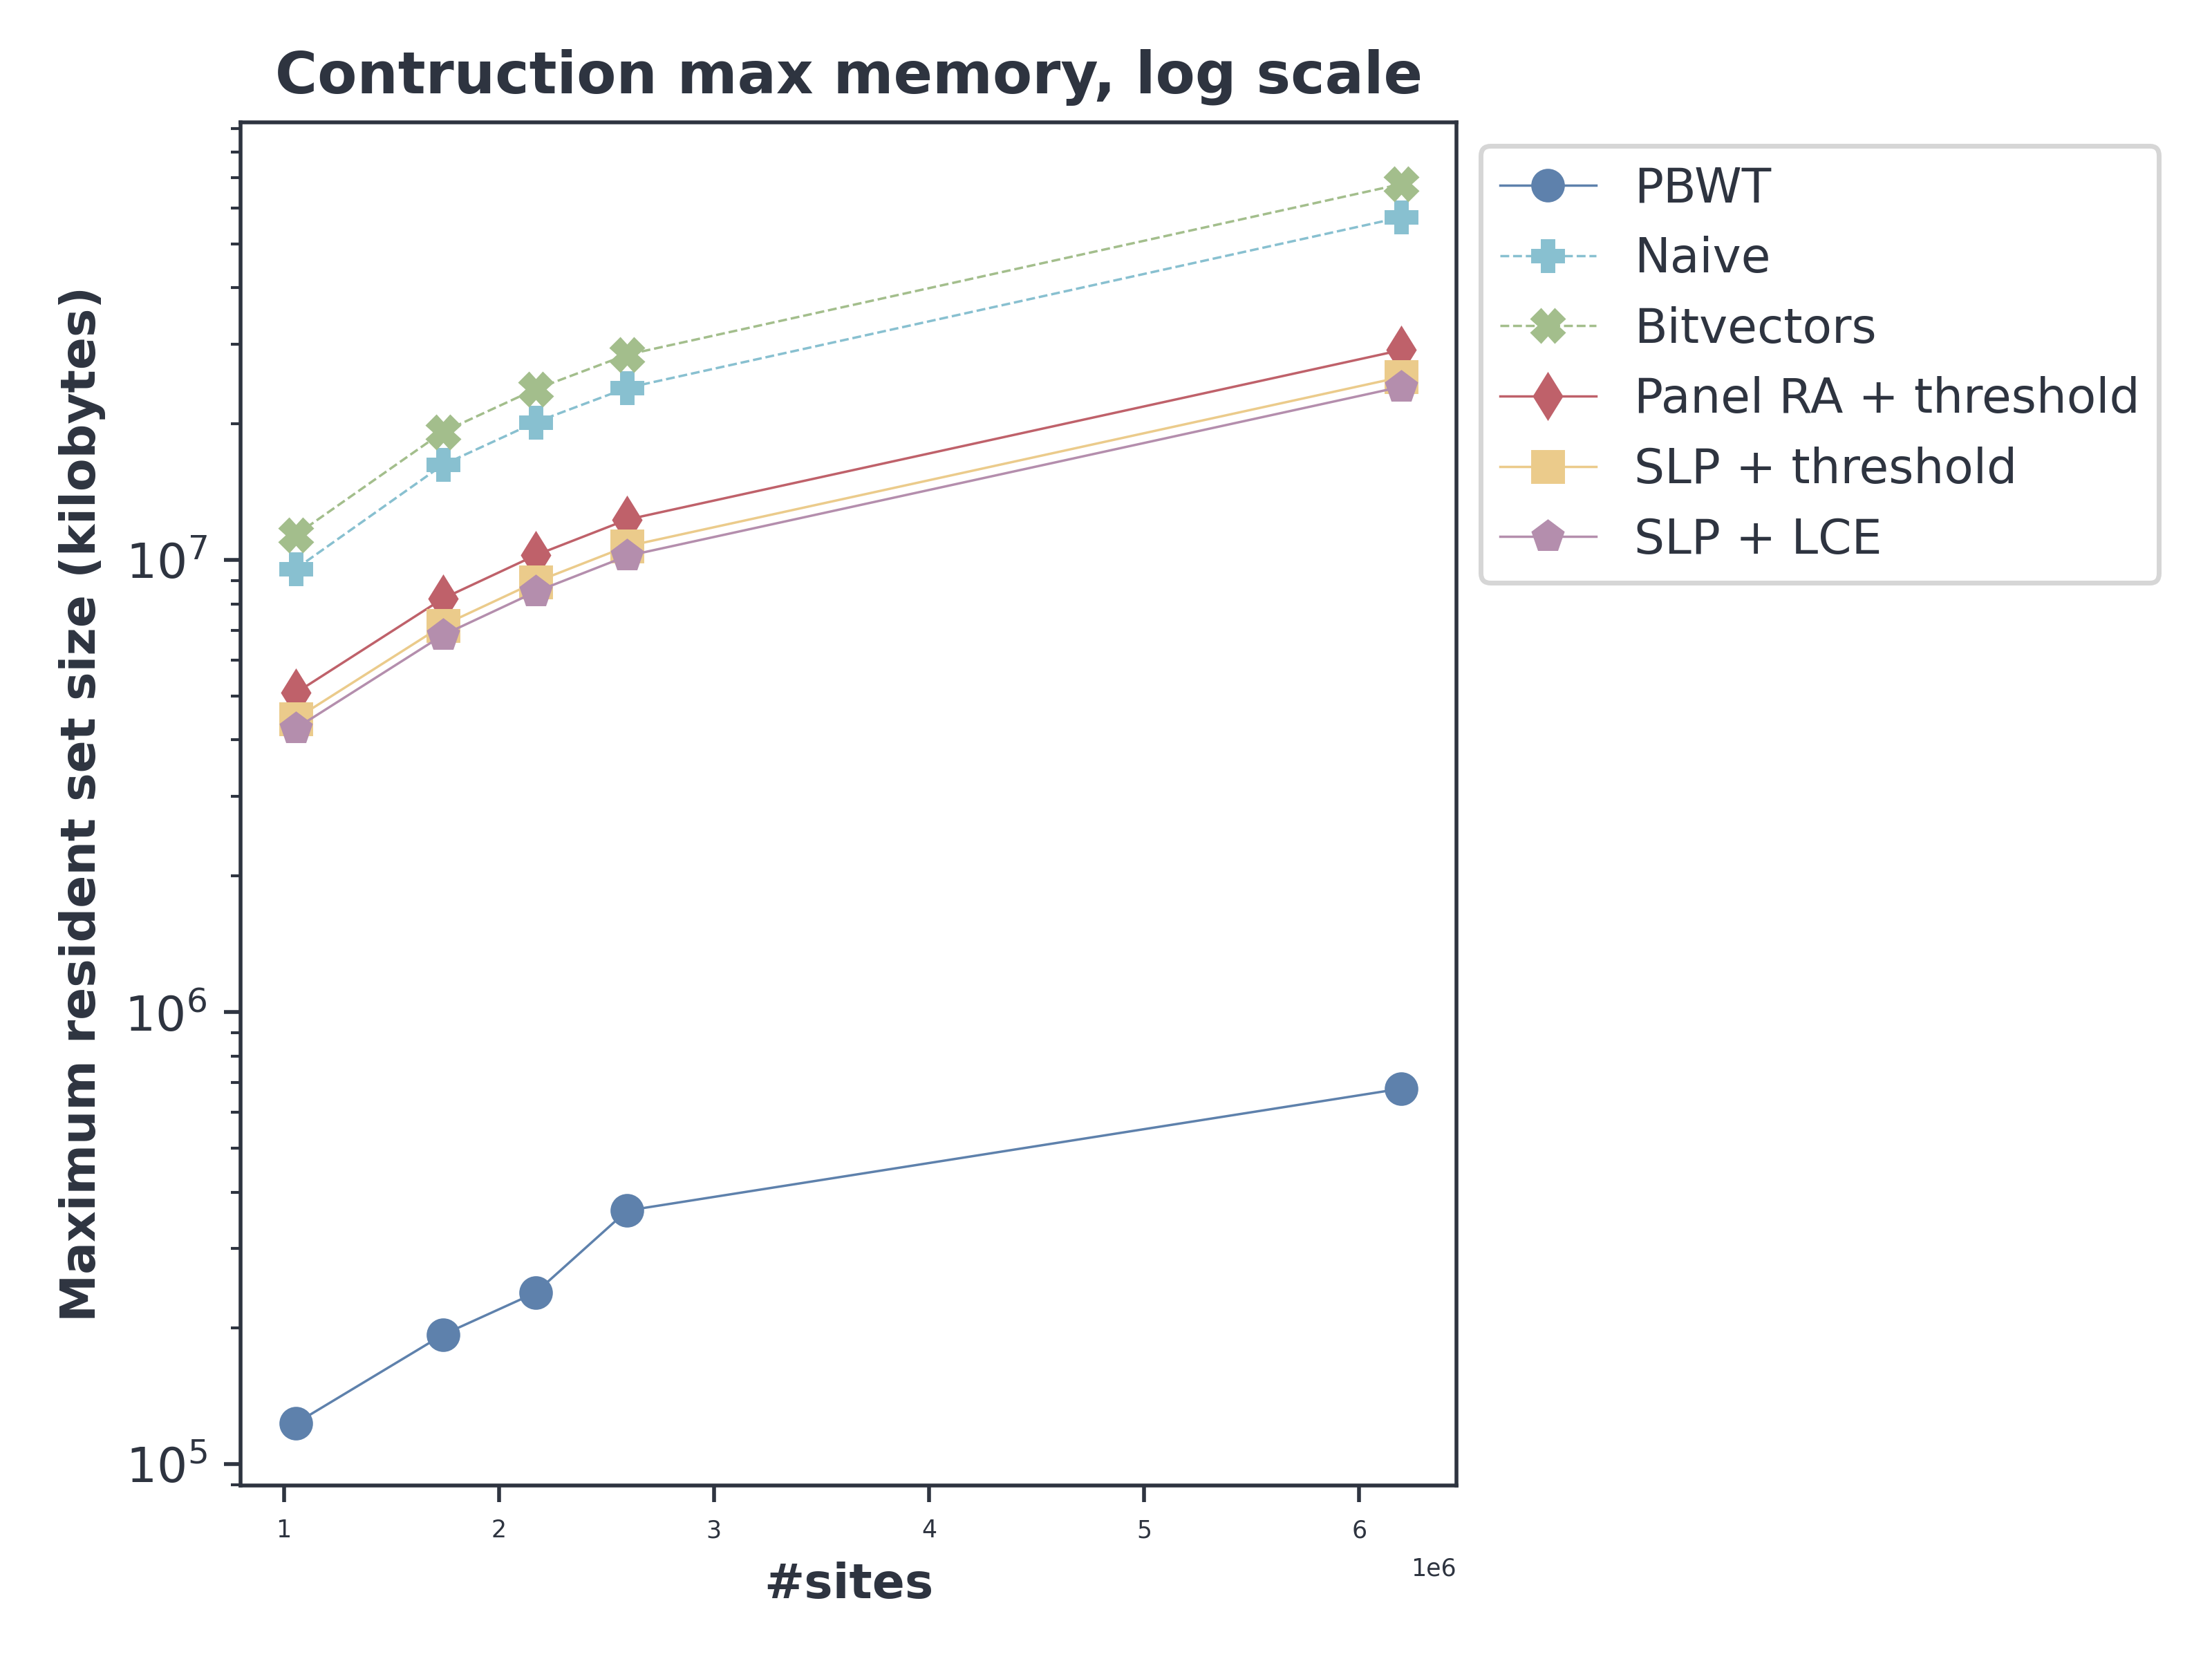
\includegraphics[width=\linewidth]{img/make_mem_log.png}
  \end{subfigure}
  \caption{Picchi di memoria per la costruzione delle varianti della RLPWBT e
    per la PBWT. Il grafico di destra presenta il tempo in scala logaritmica.}
  \label{fig:makememchr}
\end{figure}
In tabella \ref{tab:comp} si riportano, in megabytes, le dimensioni delle
singole strutture dati che compongono le varianti della \textit{RLPBWT}. Le
stesse misurazioni sono visualizzabili anche in figura \ref{fig:comp}. Si può
innanzitutto apprezzare il vantaggio dell'uso dell'\textit{SLP} rispetto al
pannello non compresso in memoria. Si può notare, inoltre, come il peso dei
bitvector sparsi per le teste di run e le threshold sia pressoché identico. Si
segnala, infine, come memorizzare i \textit{prefix array samples} e la struttura
di supporto per il calcolo delle funzioni $\varphi$ e $\varphi^{-1}$, non
presenti particolari criticità dal punto di vista della memoria richiesta.
\dc{Serve altro?}
\begin{figure}
  \centering
  \begin{subfigure}{.5\textwidth}
    \centering
    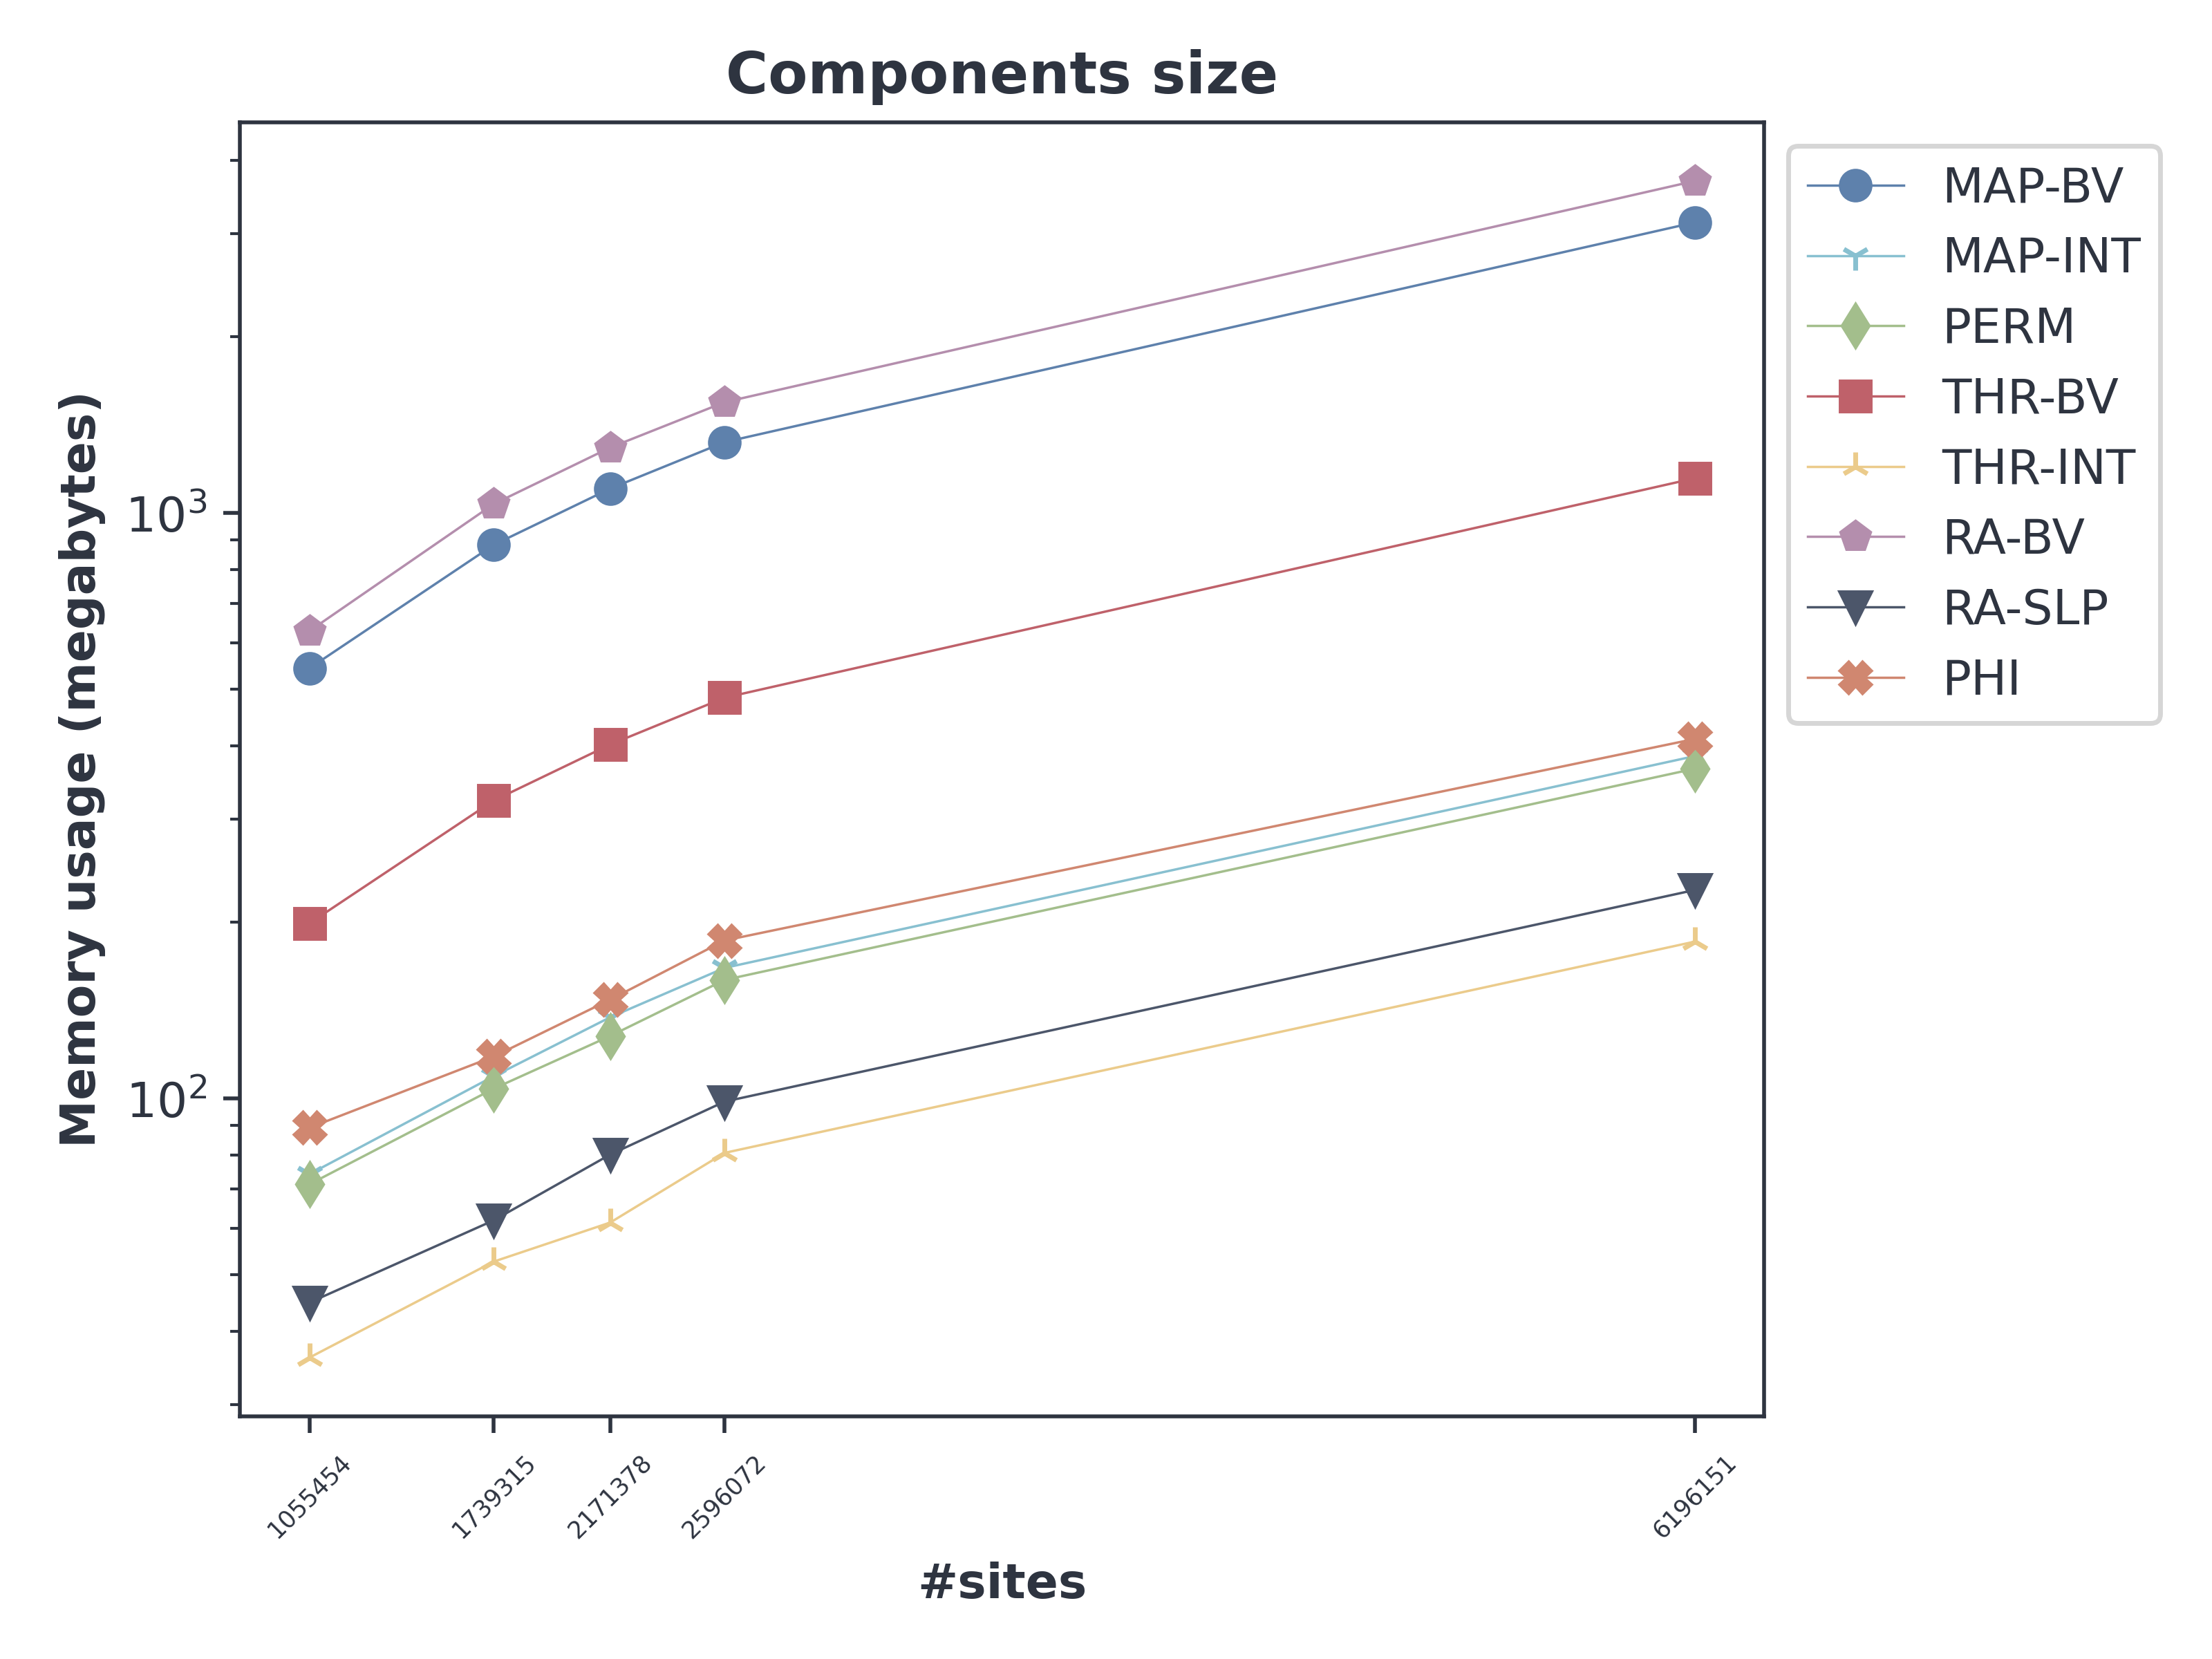
\includegraphics[width=\linewidth]{img/comp_sites.png}
  \end{subfigure}%
  \begin{subfigure}{.5\textwidth}
    \centering
    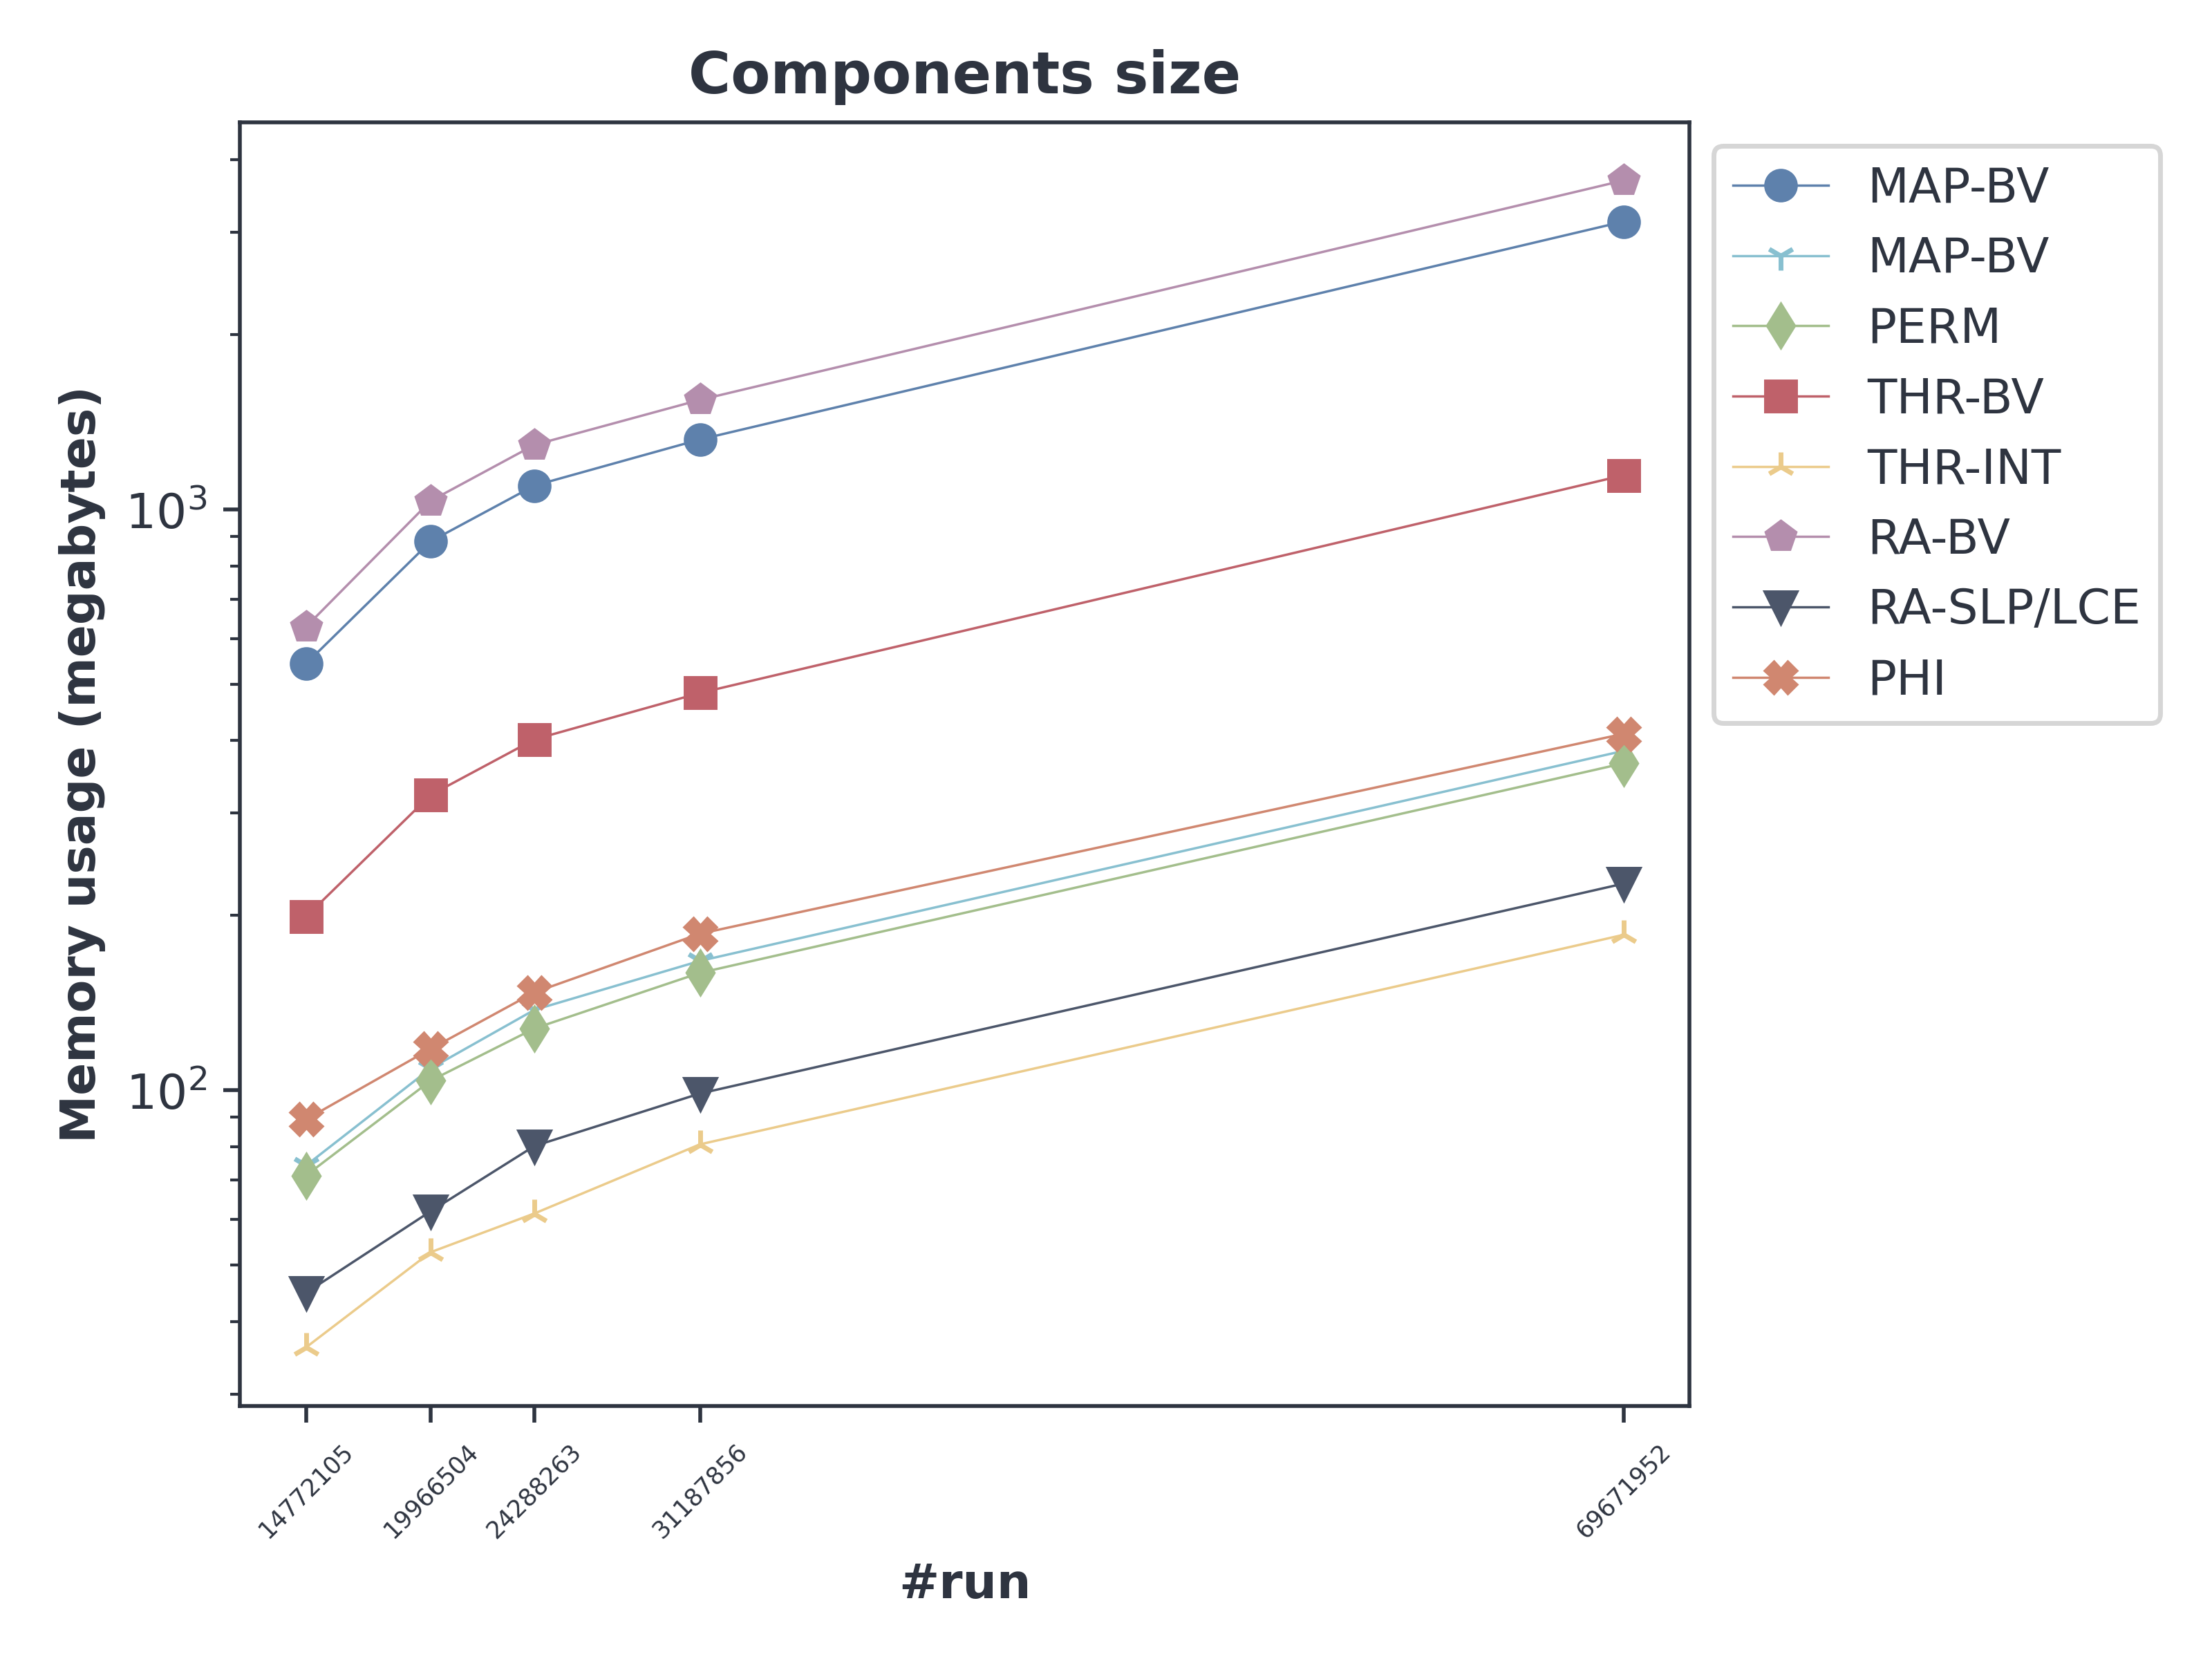
\includegraphics[width=\linewidth]{img/comp_runs.png}
  \end{subfigure}
  \caption{Memoria occupata dalle singole componenti, avendo sulle ascisse sia
    il numero di siti, a sinistra, che il numero di run, a destra. Si noti che
    con \texttt{MAP} si intende $h+u+v+c+start$ mentre con \texttt{THR} $t$. }
  \label{fig:comp}
\end{figure}
\begin{table}
  \centering
  \caption{Dimensioni, in megabytes, delle varie componenti della
    \textit{RLPBWT}.} 
  \label{tab:comp}
  \scriptsize
  \begin{tabular}{c||c|c|c|c|c|c|c|c|c}
    \textbf{Chr}  & \textbf{\textit{t}} & \textit{\textbf{Samples}} & $\boldsymbol\phi$ &
                                                                                 \textbf{SLP}
    & \textbf{Pannello} & \textbf{\textit{h}} &  \textbf{\textit{u}}  &
                                                                        \textbf{\textit{v}}
    &  \textbf{\textit{c}} +  \textbf{\textit{start}}\\ \hline    \hline
    \textbf{22}  & 198.9 & 71.3 & 89.0 & 44.7 & 628.1 & 194.5 & 180.2 & 162.7 & 5.1
    \\ \hline
    \textbf{20}  & 322.5 & 103.8 & 117.9 & 61.9 & 1035.1 & 315.1 &  293.5 & 264.7 & 8.3
    \\ \hline
    \textbf{18}  & 401.9 & 127.8 & 147.4 & 80.2 & 1292.2 & 392.9 & 366.1 & 330.4 & 10.3
    \\ \hline
    \textbf{16}  & 483.4 & 159.3 & 186.1 & 98.7 & 1544.9 & 472.4 & 439.5 & 396.1 & 12.4
    \\ \hline
    \textbf{1}  & 1145.6 & 365.6 & 410.9& 226.9 & 3687.3 & 1119.6 & 1043.4 & 940.4 & 29.5
    \\ 
  \end{tabular}
\end{table}
% \begin{table}
%   \centering
%   \caption{Dimensioni, in megabytes, delle varie componenti della
%     \textit{RLPBWT}.} 
%   \label{tab:comp}
%   \scriptsize
%   \begin{tabular}{|c|c|c||c|c|c|c|c|c|c|c|c|}
%     \hline
%     Chr & Sites & Runs & h+u+v & t & samples & $\phi$ & slp & panel & h & u
%     & v \\ \hline
%     22 & 1055454 & 14772105 & 537.4 & 198.9 & 71.3 & 89.0 & 44.7
%        & 628.1 & 194.5 & 180.2 & 162.7 \\ \hline
%     20 & 1739315 & 19966504 & 873.2 & 322.5 & 103.8 & 117.9
%                                                       & 61.9 & 1035.1 & 315.1 & 293.5 & 264.7 \\ \hline
%     18 & 2171378 & 24288263 & 1089.298 & 401.9 & 127.8 & 147.4
%                                                       & 80.2 & 1292.2 & 392.9 & 366.1 & 330.4 \\ \hline
%     16 & 2596072 & 31187856 & 1307.931 & 483.4 & 159.3 & 186.1
%                                                       & 98.7 & 1544.9 & 472.4 & 439.5 & 396.1 \\ \hline
%     1 & 6196151 & 69671952 & 3103.508 & 1145.6 & 365.6 & 410.9
%                                                       & 226.9 & 3687.3 & 1119.6 & 1043.4 & 940.4 \\ \hline 
%   \end{tabular}
%\end{table}
\paragraph{Calcolo degli SMEM}
Passando all'effettivo calcolo degli SMEM, si possono, anche in questo caso,
confermare i risultati avuti con i pannelli simulati.\\
In figura \ref{fig:smemtimechr} si riportano i risultati i termini di tempo di
calcolo, notando che:
\begin{itemize}
  \item come atteso, l'algoritmo \textit{PBWT Dynamic} risulta essere il più
  performante
  \item la \textit{RLPBWT} con \textit{SLP} e \textit{threshold}, a causa dei
  frequenti accessi all'\textit{SLP}, sia per il calcolo delle lunghezze delle
  matching statistics che per la fase di ``disambiguazione'', richiede più tempo
  di tutte le altre varianti, soprattutto se si pensa alla corrispondente
  variante senza \textit{SLP}
  \item  la \textit{RLPBWT} con \textit{SLP} e \textit{LCE} risulta essere circa
  il doppio più lenta della soluzione proposta da Durbin con l'\textit{algoritmo
    5}. Questo è un risultato 
  molto interessante se si tiene in considerazione la memoria necessaria per il
  calcolo degli SMEM
\end{itemize}
\begin{figure}
  \centering
  \begin{subfigure}{.5\textwidth}
    \centering
    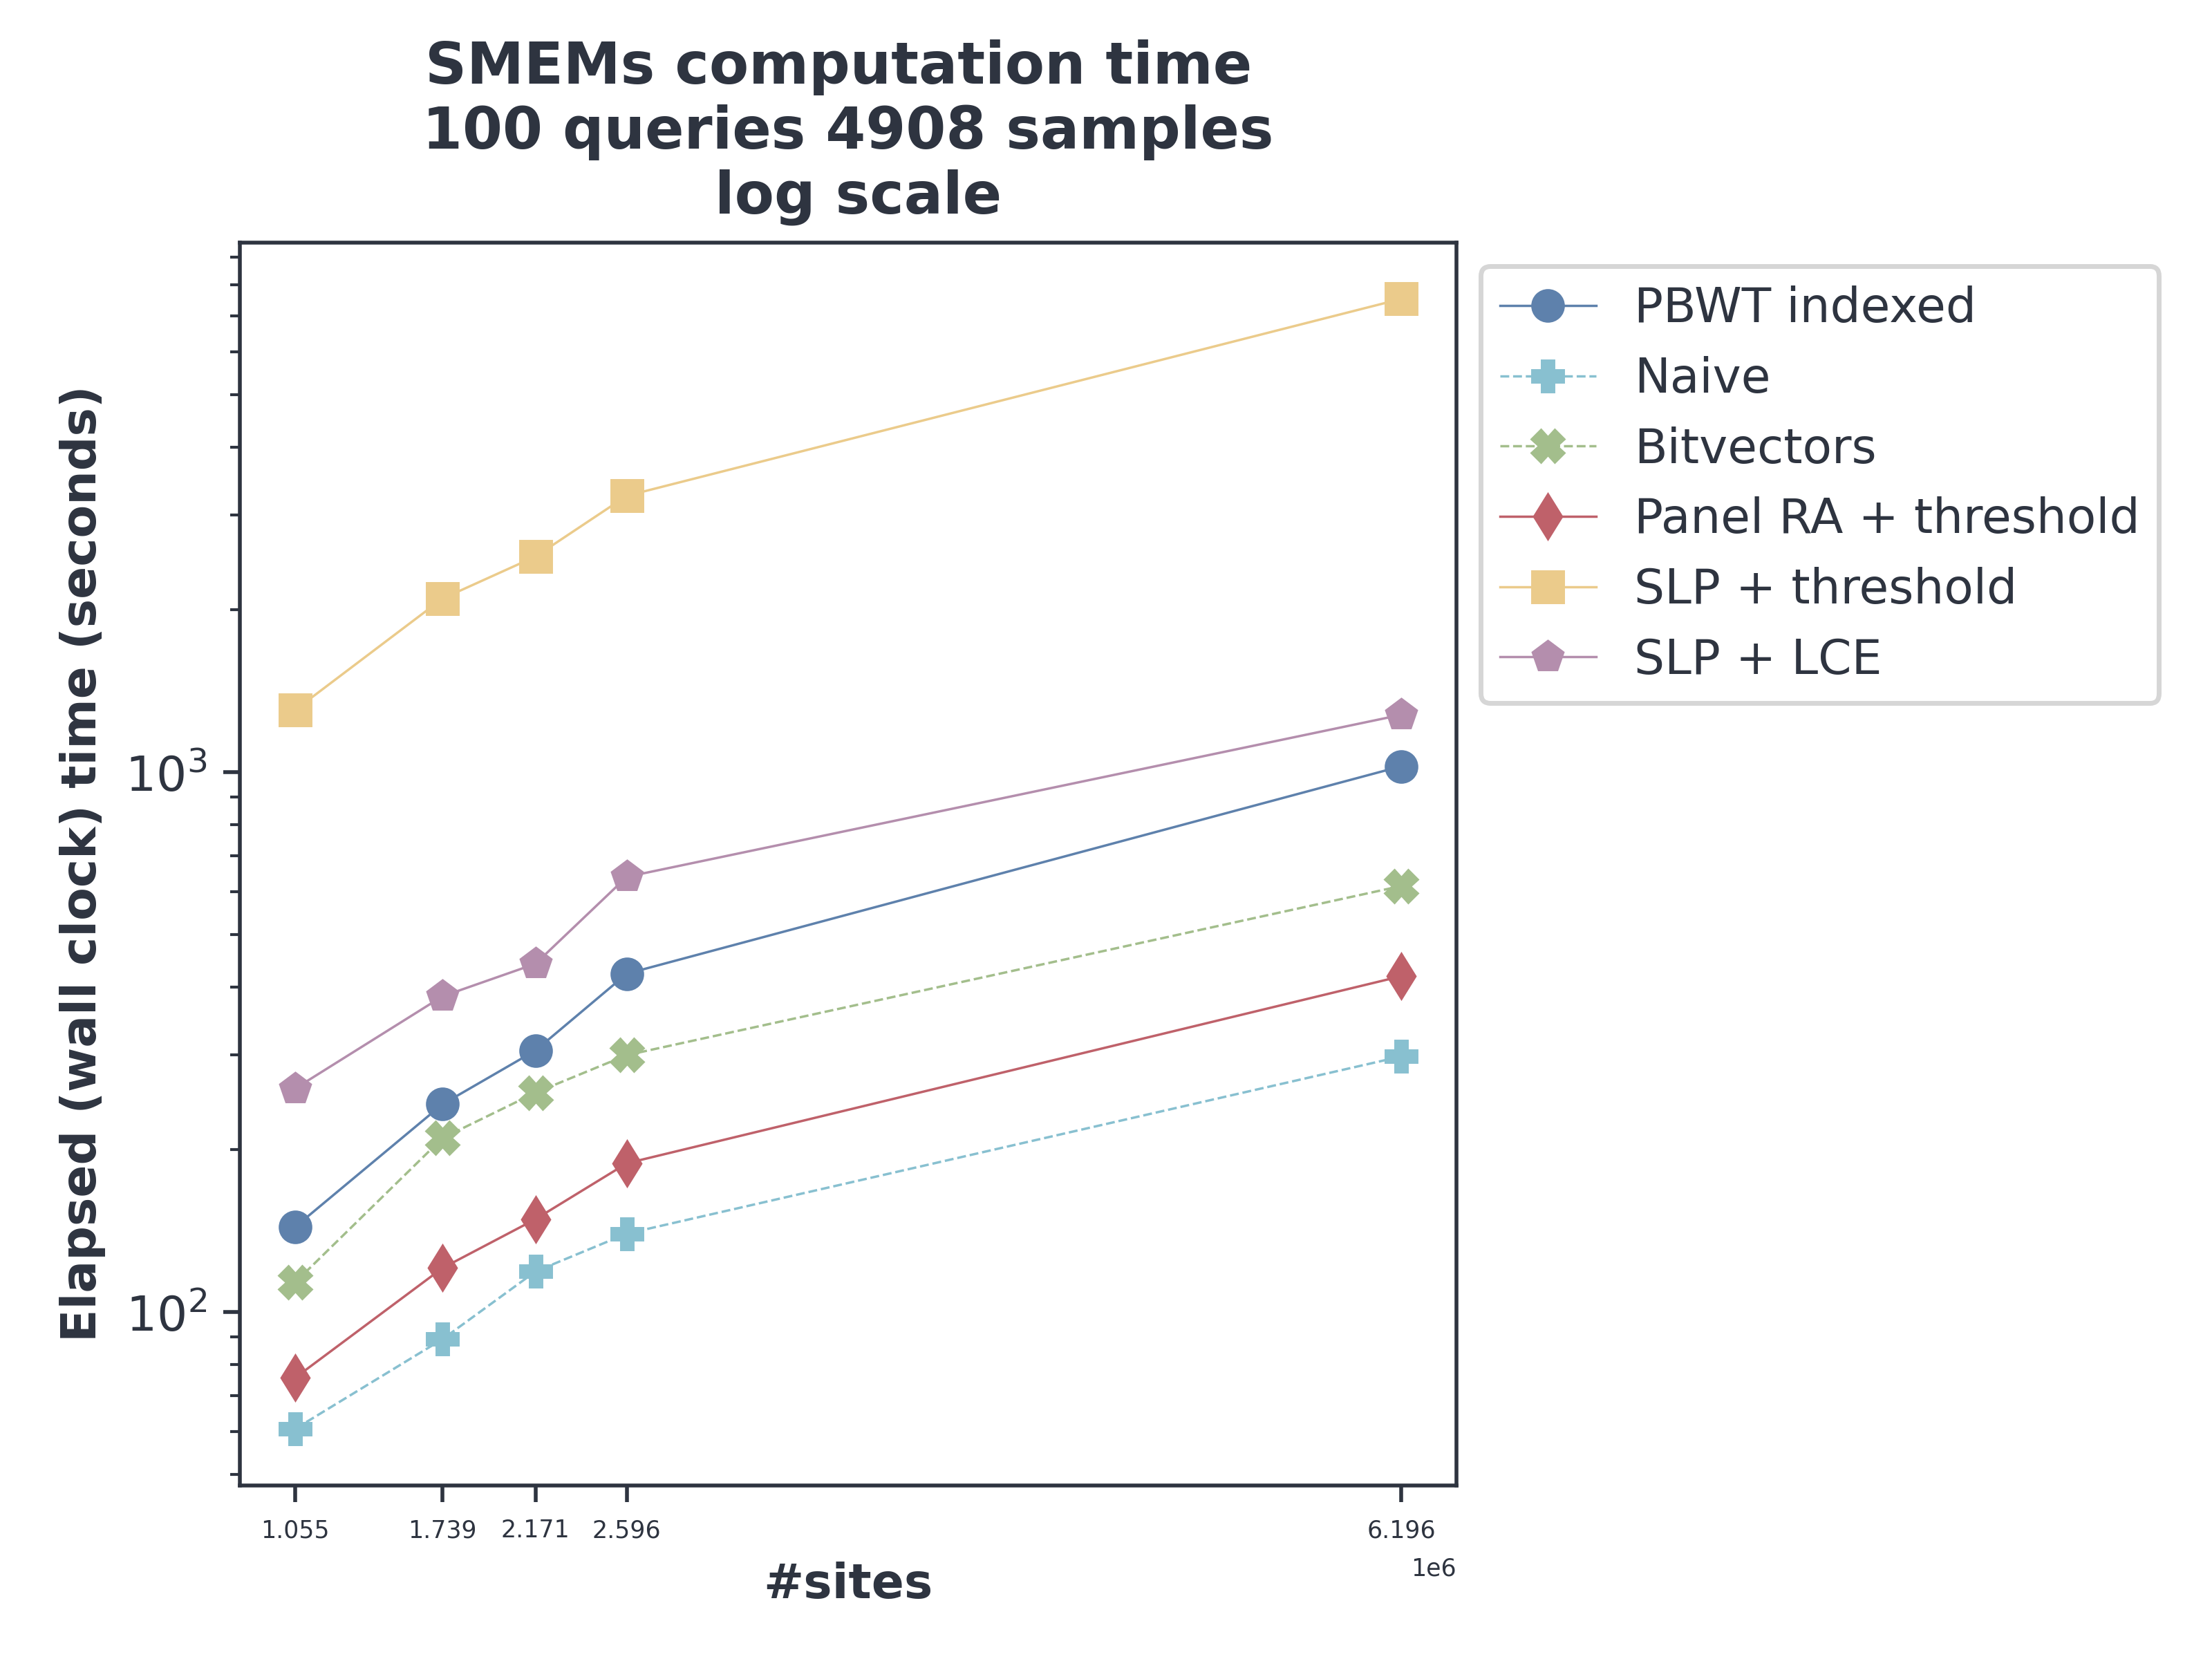
\includegraphics[width=\linewidth]{img/exe_time_log.png}
  \end{subfigure}%
  \begin{subfigure}{.5\textwidth}
    \centering
    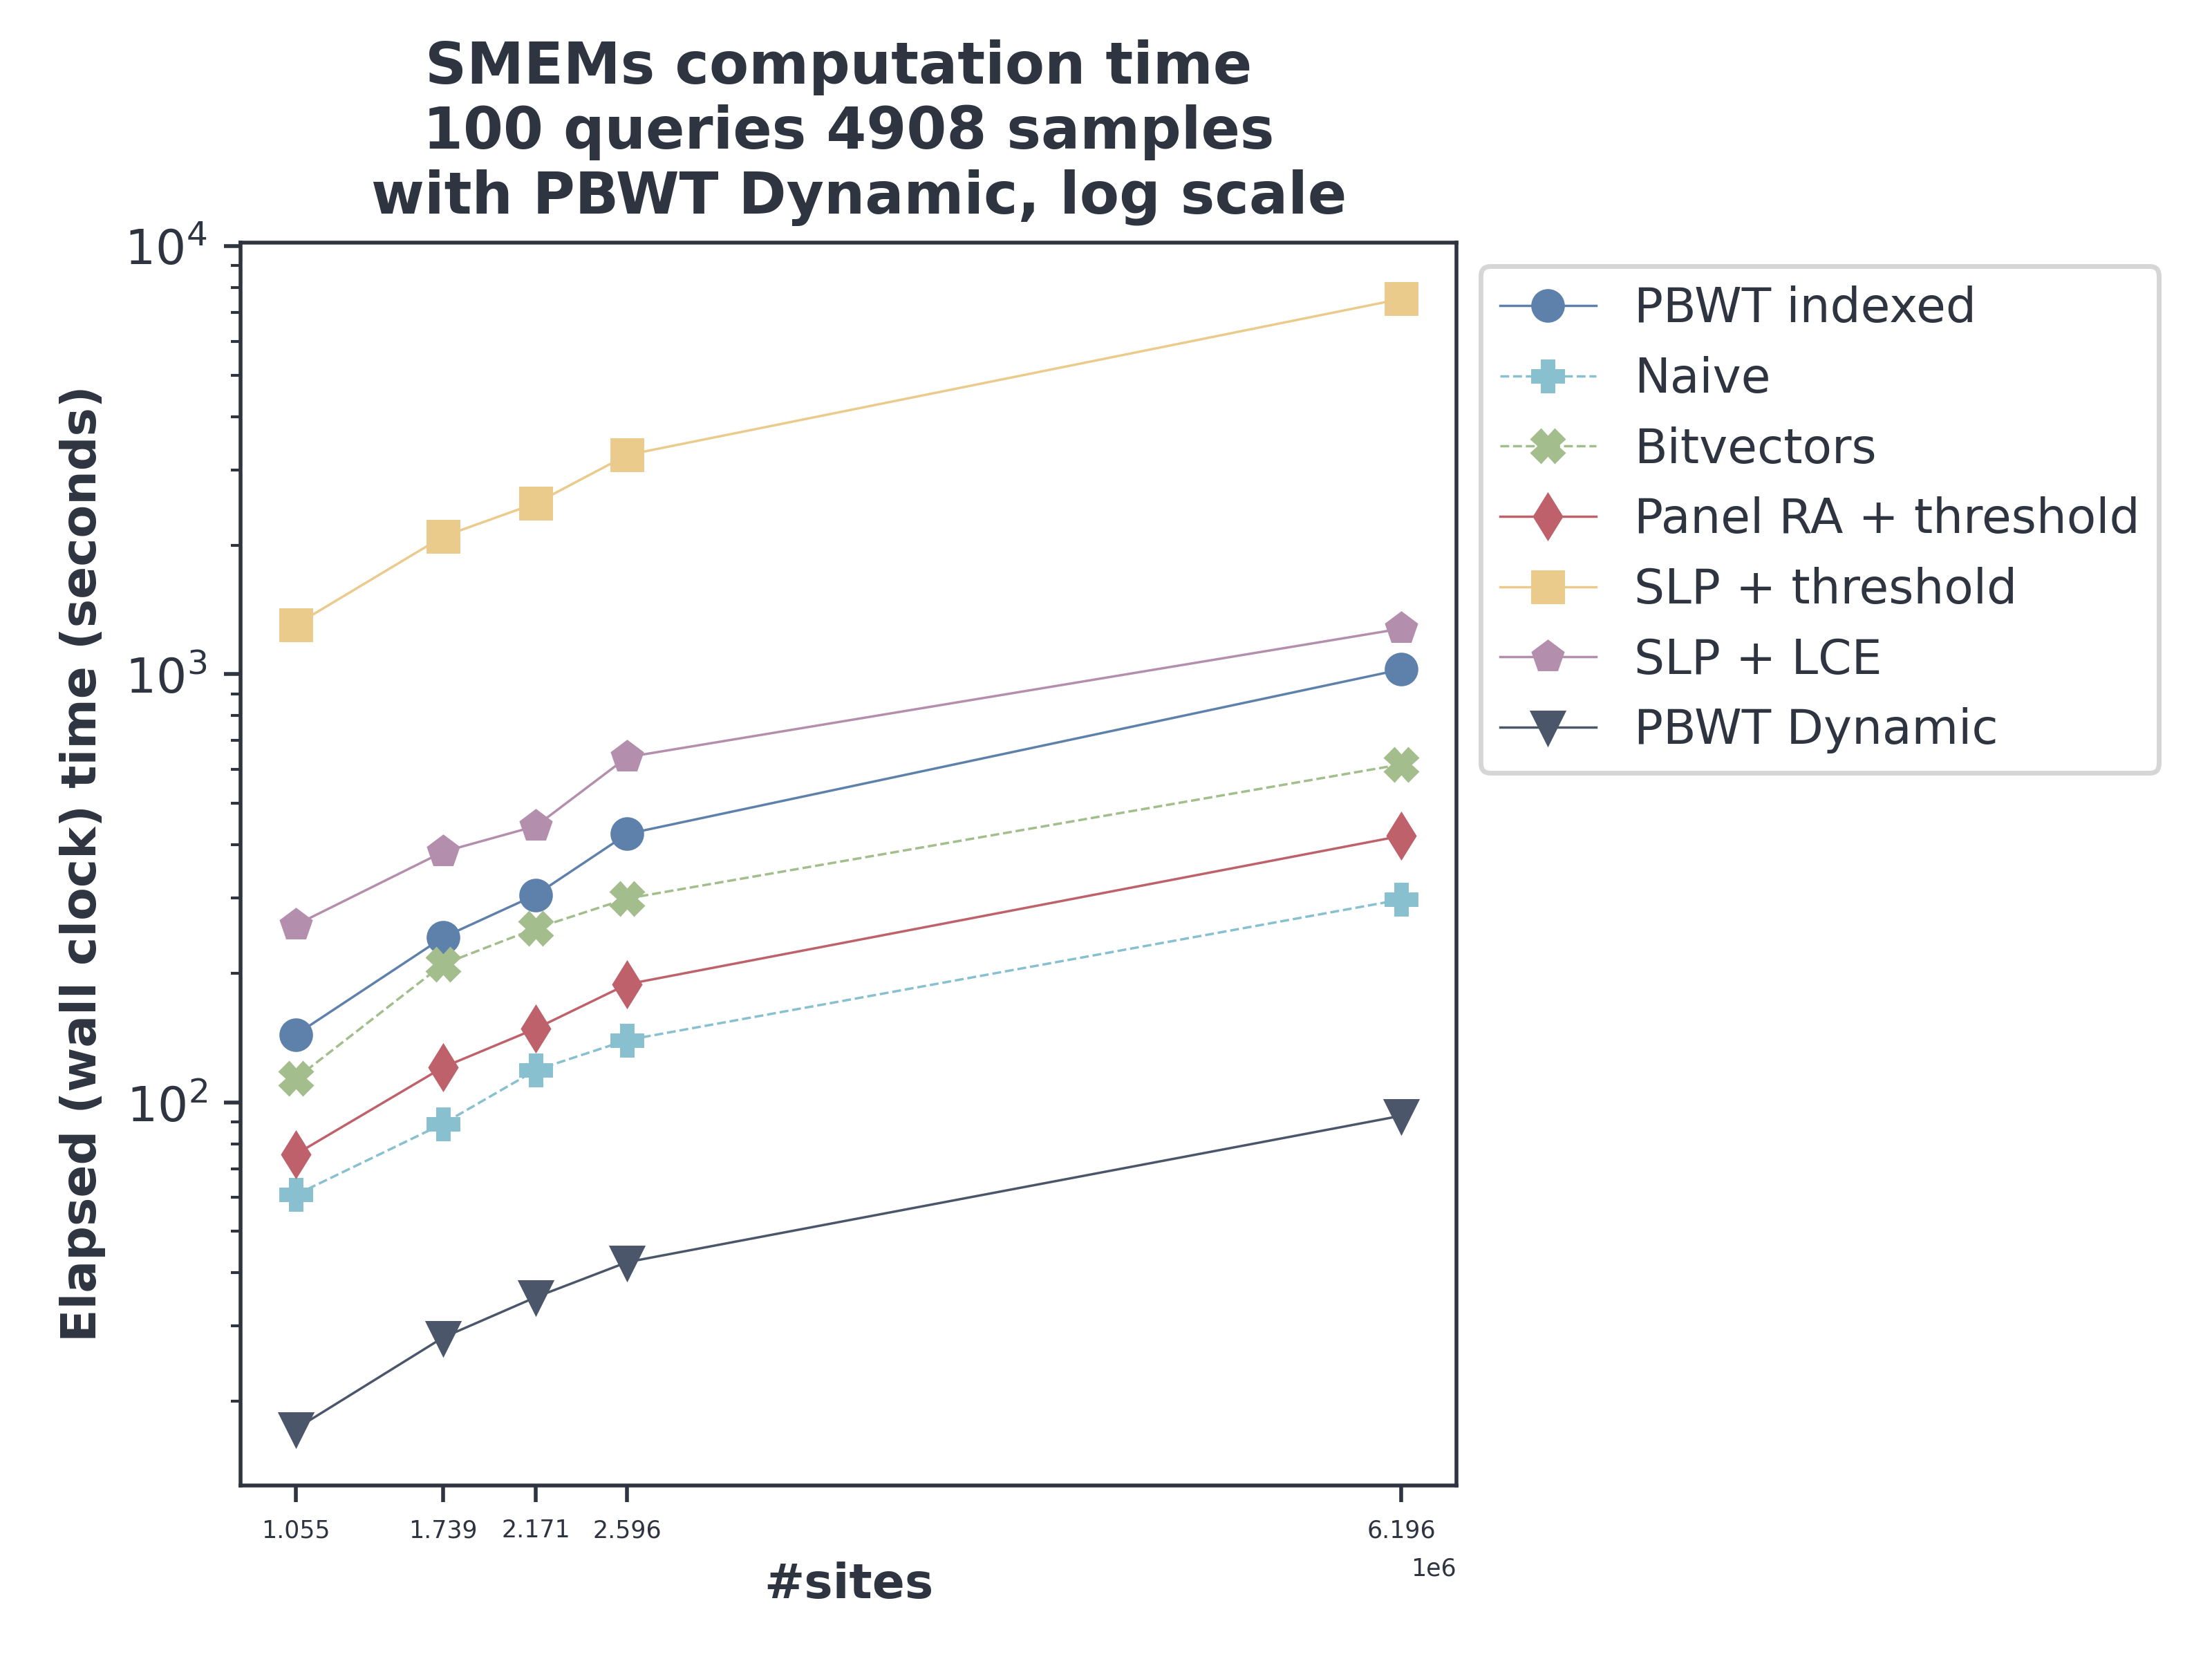
\includegraphics[width=\linewidth]{img/exe_time_dyn_log.png}
  \end{subfigure}
  \caption{Tempo di calcolo degli SMEM, in scala logaritmica, con e senza
    l'algoritmo \textit{PBWT Dynamic}.}
  \label{fig:smemtimechr}
\end{figure}
In figura \ref{fig:smemmemchr} si riportano i risultati i termini di picchi di
memoria durante la computazione degli SMEM. Anche in questo caso, si possono fare
diverse osservazioni:
\begin{itemize}
  \item come previsto, la \textit{PBWT Dynamic} ha le migliori prestazioni anche
  in spazio, calcolando dinamicamente i vari indici per il computo dei match
  massimali interni al pannello
  \item l'\textit{algoritmo 5} di Durbin conferma le previsioni fatte
  dall'autore, avendo che la memoria utilizzata è circa $13NM$ bytes
  \item la differenza tra le varianti della RLPBWT basate sul calcolo dell'array
  delle Matching Statistics è minima. All'aumentare delle dimensioni del
  pannello, d'altro canto, si prevede che l'uso dell'SLP garantisca un minor uso
  di memoria
\end{itemize}
\begin{figure}
  \centering
  \begin{subfigure}{.5\textwidth}
    \centering
    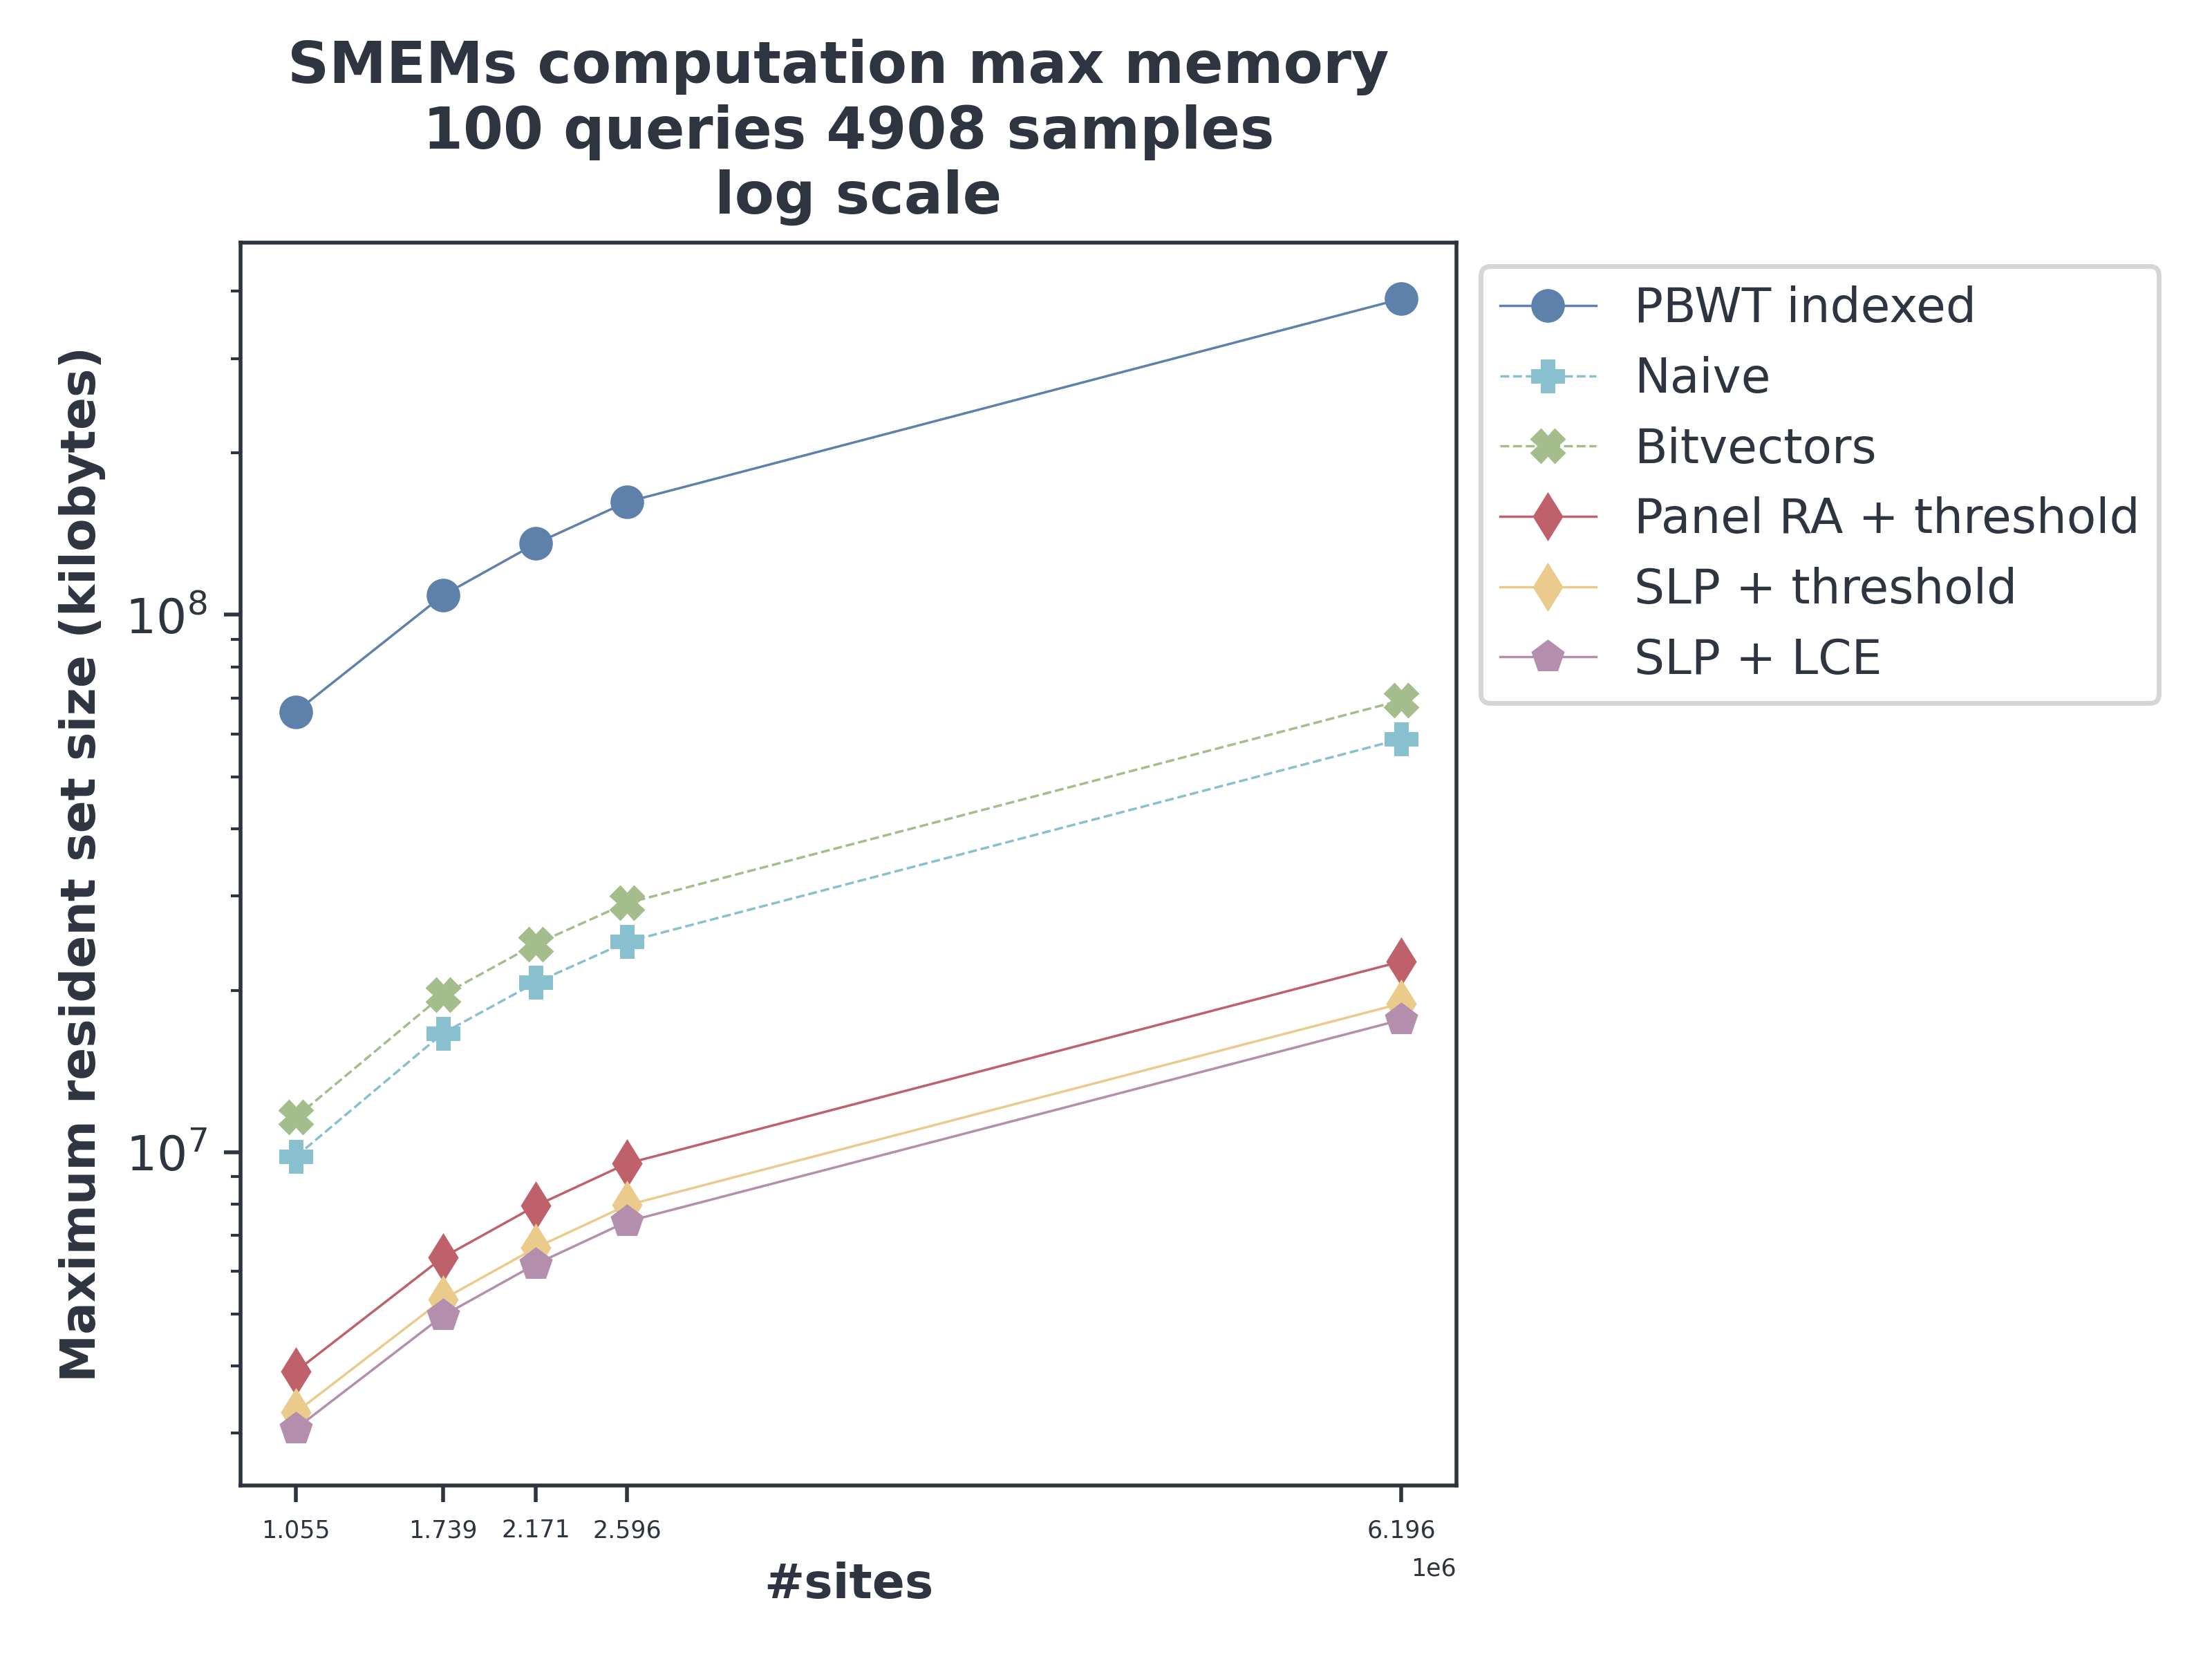
\includegraphics[width=\linewidth]{img/exe_mem_log.png}
  \end{subfigure}%
  \begin{subfigure}{.5\textwidth}
    \centering
    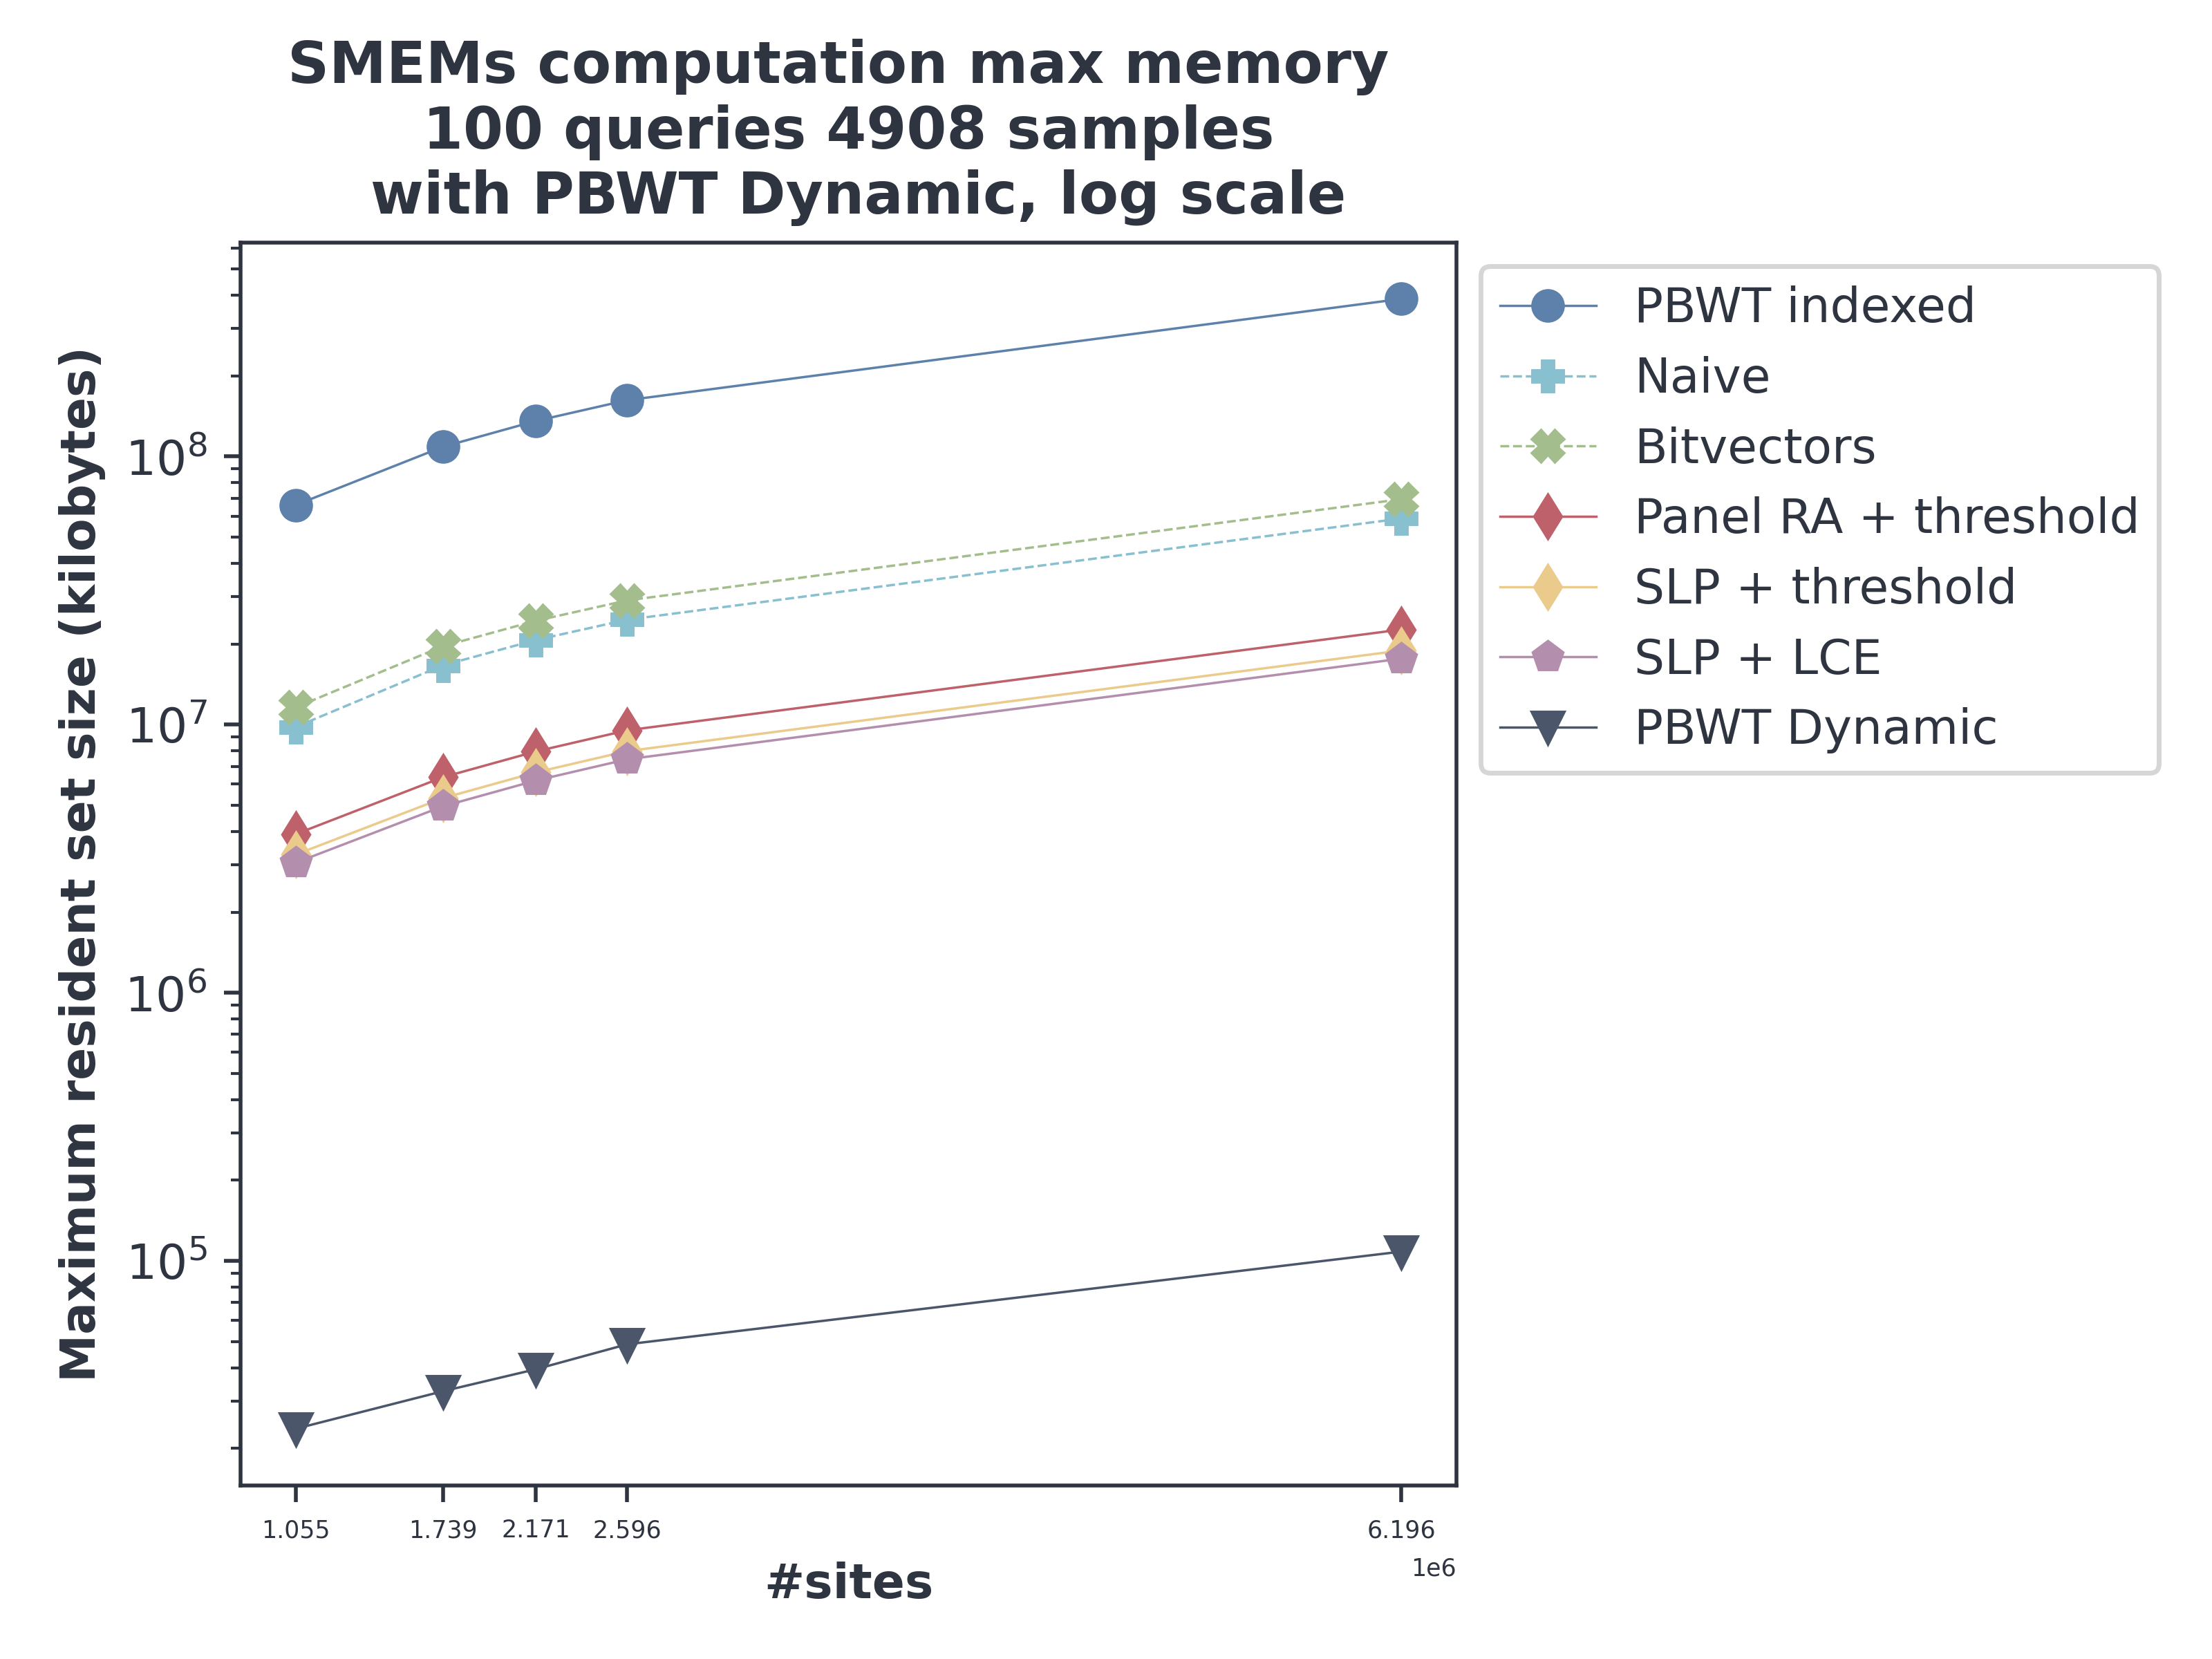
\includegraphics[width=\linewidth]{img/exe_mem_dyn_log.png}
  \end{subfigure}
  \caption{Picchi di memoria per il calcolo degli SMEM, in scala logaritmica,
    con e senza 
    l'algoritmo \textit{PBWT Dynamic}.}
  \label{fig:smemmemchr}
\end{figure}
Interessante è notare il rapporto tra la memoria richiesta dalla \textit{RLPBWT}
con \textit{SLP} e \textit{LCE} e la \textit{PBWT Indexed}:
\begin{table}[H]
  \centering
  \footnotesize
  \begin{tabular}{c|c|c|c|c}
    \textbf{\#Samples} & \textbf{\#Siti}
    & \textbf{RLPBWT SLP-LCE (\textit{kb})}
    & \textbf{PBWT Indexed (\textit{kb})} & \textbf{\%}\\
    \hline
    4908 & 1055454 & 3058088 & 65975520 & 4.64\\
    4908 & 1739315 & 4961664 & 108713424 & 4.56\\
    4908 & 2171378 & 6190684 & 135726084 & 4.56\\
    4908 & 2596072 & 7430300 & 162257008 & 4.58\\
    4908 & 6196151 & 17635700 & 387252160 & 4.55
  \end{tabular}
\end{table}
Anche in questo caso le percentuali risultano leggermente peggiori rispetto ai
pannelli simulati, pur restando risultati molto interessanti.
\subsection{Tempo di una singola query}
Infine, per completare lo studio delle prestazioni temporali, si è deciso di
isolare il calcolo degli SMEM con ogni singola query, valutando media e
deviazione standard delle 100 query. Tale risultato è visualizzabile in figura
\ref{fig:smemsinglechr}, dove si è deciso di escludere la \textit{RLPBWT
  na\"{i}ve} e la \textit{RLPBWT con bitvector} in quanto non in grado di
computare quali righe presentino un certo SMEM, e conferma quanto ipotizzato e
discusso precedentemente: 
\begin{itemize}
  \item la \textit{PBWT Dynamic} richiede di costruire, ogni volta, la
  trasformata della query e
  calcolare i match interni al pannello originale a cui viene
  aggiunta la query, considerando poi solo i match provenienti da tale
  pannello. Questo processo richiede molte operazioni e non è ottimizzato per 
  una singola query. Una query o un centinaio di query hanno quindi all'incirca
  lo tempo di calcolo
  \item la \textit{PBWT Indexed} richiede molto meno operazioni ed è quindi la
  soluzione più performante
  \item per quanto riguarda la \textit{RLPBWT} con \textit{SLP} e
  \textit{threshold}, ovvero quella più lenta, si ha che essa soffre
  degli stessi problemi relativi all'random access, precedentemente
  descritti. Questi problemi sono risolti dalla \textit{RLPBWT} con
  \textit{pannello completo} e \textit{threshold}
  \item  utilizzando le \textit{LCE query} si ha una soluzione leggermente più
  lenta rispetto alla \textit{RLPBWT} con
  \textit{pannello completo} e \textit{threshold}, dovuto, di fatto, ai costi
  di calcolo delle \textit{LCE query} stesse
\end{itemize}
Tali risultati sono ottenuti isolando unicamente le singole funzioni atte al
calcolo dei match, escludendo i tempi di caricamento delle strutture o di
eventuali ulteriori costruzioni (come degli array nel caso della \textit{PBWT
  indexed} o della \textit{PBWT} della singola query nel caso della \textit{PBWT
Dynamic}).
\begin{figure}
  \centering
  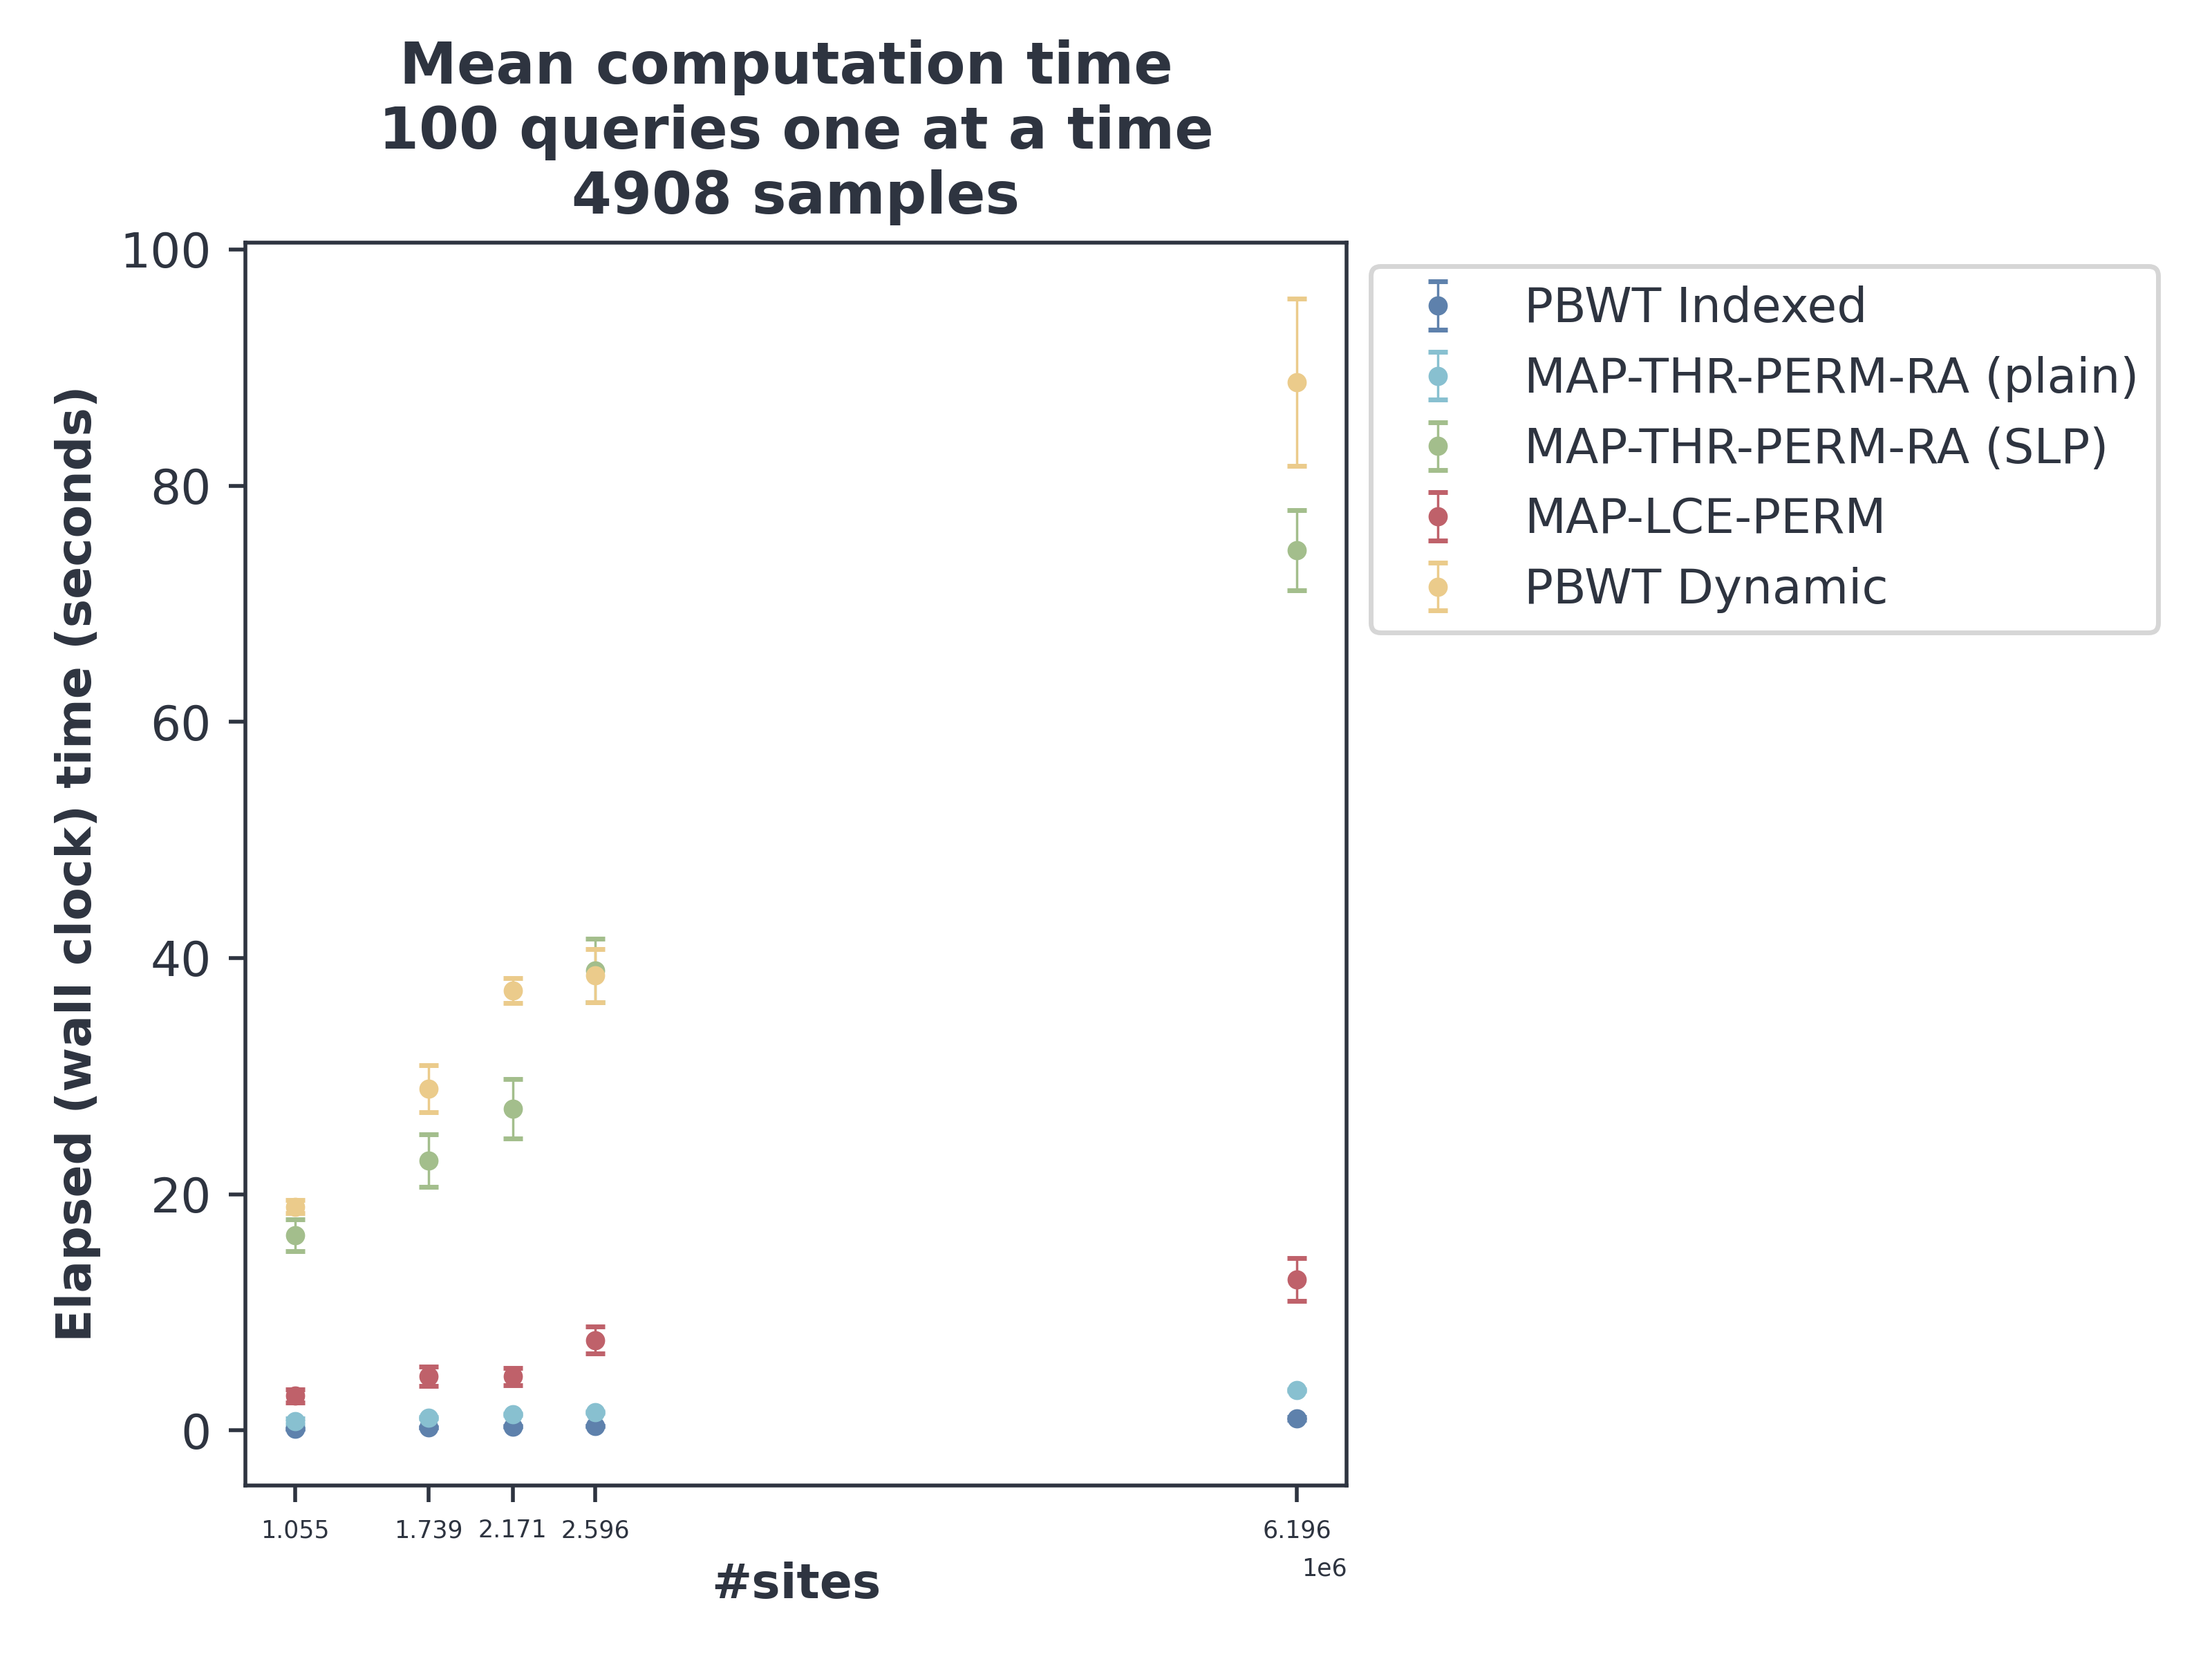
\includegraphics[width=0.5\textwidth]{img/exe_single_time_dyn_paper.png}
  \caption{Tempo medio di esecuzione del calcolo degli SMEM per una singola
    query. Il grafico di destra è in scala logaritmica e, in entrambi, le
    barre d'errore rappresentano la deviazione standard.}
  \label{fig:smemsinglechr}
\end{figure}
% LocalWords:  sottostrutture
